\documentclass{article}
\linespread{1.5}
\usepackage[T1]{fontenc}
\usepackage{ctex}
\usepackage{esvect}
\usepackage{arydshln}
\usepackage{mathrsfs}
\usepackage{amsmath}
\numberwithin{equation}{section}
\numberwithin{figure}{section}
\usepackage{caption}
\usepackage{graphicx, subfig}
\usepackage{fontspec} 
% \setmainfont{Times New Roman}
% \setCJKmainfont{SimSun}
\usepackage{newtxtext}
\usepackage[colorlinks,linkcolor=black,anchorcolor=blue,citecolor=green]{hyperref}
\usepackage{geometry}
\usepackage{lipsum} % 该宏包是通过 \lipsum 命令生成一段本文,正式使用时不需要引用该宏包
\usepackage[dvipsnames,svgnames]{xcolor}
\usepackage[strict]{changepage} % 提供一个 adjustwidth 环境
\usepackage{framed} % 实现方框效果
\usepackage{tcolorbox}
\tcbuselibrary{skins, breakable, theorems}
\NewTcbTheorem[number within=section]{Definition}{定义}{colback=green!5,colframe=green!35!black,fonttitle=\bfseries}{def}

\geometry{a4paper,centering,scale=0.8}
% environment derived from framed.sty: see leftbar environment definition
\definecolor{formalshade}{rgb}{0.95,0.95,1} % 文本框颜色
% ------------------******-------------------
% 注意行末需要把空格注释掉,不然画出来的方框会有空白竖线
\newenvironment{formal}{%
\def\FrameCommand{%
\hspace{1pt}%
{\color{DarkBlue}\vrule width 2pt}%
{\color{formalshade}\vrule width 4pt}%
\colorbox{formalshade}%
}%
\MakeFramed{\advance\hsize-\width\FrameRestore}%
\noindent\hspace{-4.55pt}% disable indenting first paragraph
\begin{adjustwidth}{}{7pt}%
\vspace{2pt}\vspace{2pt}%
}
{%
\vspace{2pt}\end{adjustwidth}\endMakeFramed%
}
% ------------------******-------------------
\CTEXoptions [today = old]
\title{Modern Control Engineering}
\author{Katsuhiko Ogata}% 用 and 分隔多个作者
\date{\today}
\begin{document}
\maketitle

\newpage

\section{控制工程引言}
\subsection{控制理论历史发展}
\begin{itemize}
    \item 十八世纪,James Watt发明了用于控制蒸汽机速度控制的centrifugal governor,这是第一个自动控制的成果。
    \item 1922年,Minorsky提出了怎么通过描述系统的微分方程确定系统稳定性。
    \item 1932年,Nyquist提出了基于输入为稳态正弦信号的开环响应的确定闭环系统稳定性的相对简单的分析过程。
    \item 1934年,Hazen提出了servomechanisms。
    \item 1940-1950年,频率响应和波特图的提出,使得设计满足性能需求的线性闭环控制系统变得可能。
    \item 1950-1960年,根轨迹root-locus方法被全面发展。
    \item 1980-2000年,现在控制工程的理论聚焦于robust control发展。
\end{itemize}
\subsection{控制理论类别}
\begin{formal}
    \item 经典控制理论(Classical control theory):只能够处理单个输入单个输出的控制理论,其核心为频率响应法(frequency-response and root-locus methods)和根轨迹法。然而这种方法设计出的系统能够满足需求但并不是最优的。
    \item 
\end{formal}
\begin{formal}
    \item 现代控制理论(Modern control theory):能够处理多个输入多个输出的复杂系统的控制理论,其核心为时域分析(time-domain analysis)和状态变量综合(synthesis using state variables)。这种方法设计出复杂的、要求严苛的系统。然而这种方法设计出的系统的稳定性对于“所使用的模型和实际系统的误差“十分敏感,因此在使用这个方法进行设计时,一般会提前设定好误差区间,只要实际系统与模型的误差在误差区间范围内,所设计的系统就能保持稳定。
    \item 鲁棒控制理论(Robust control theory):基于上述原理的设计方法就称为robust control theory,这一理论同时采用了频率响应方法和时域分析方法。
\end{formal}
\subsection{基本术语定义}
\begin{formal}
    \item Controlled Variable:应变量,一般指系统的输出。
    \item Control Signal or Manipulated variables:自变量,即影响应变量(Controlled Variable)的值的量。
    \item Control:根据应变量的值,调整变量以限制或纠正应变量与其理想值的偏移。
    \item Plants:能够实现某种特定操作的事物,可以是某一个设备,也可以是一套机器,本书中任何受控的物体都被称为plant。
    \item Process:任何受控的操作称为process。
    \item Systems:由多个组成部分相结合实现某一功能的事物称为System。
    \item Disturbance:对输出起副作用的信号;系统内部的称为internal,系统外部的称为external。
    \item Feedback Control:根据输出与参考值的差异进而控制输出以降低Disturbance对输出造成的影响。
    \item 
\end{formal}
实现某一功能的组合称为System,这一组合的输入(自变量)称为Control Signal or Manipulated Variable,这一组合的输出称为Controlled Variable;这个组合中的每个部分称为Plant,每个Plant实现的功能称为Process;使得系统的输出非理想的量称为Disturbance,根据输出的非理想程度对输出进行调整以恢复理想情况降低Disturbance影响的过程称为Feedback Control。
\subsection{闭环控制和开环控制}
\begin{formal}
    \item Feedback Control Systems:通过输出和参考输入的差值对系统进行控制以保持系统的输出和参考输入之间保持预设关系的系统。
    \item Closed-Loop Control Systems:Feedback Control Systems一般就是指closed-loop control system,这两个定义基本相同。
    \item Open-Loop Control Systems:输出不会与参考输入相比较、无法产生任何control行为的系统,即系统无法根据系统的输出对其进行调整。开环系统通常工作在确定的工作状态,不会因为输出的改变而改变,一般这种系统都是基于时域的系统,根据设定好的时序关系进行工作。
    \item 
\end{formal}
闭环系统和开环系统的优劣势分析:
\begin{itemize}
    \item 抗干扰能力:闭环系统抗干扰能力强;开环系统抗干扰能力弱。
    \item 系统稳定性:闭环系统稳定性差,容易因为overcorrect导致震荡;开环系统稳定性好。
    \item 成本和功率需求:闭环系统结构更复杂,相较开环系统成本更高;开环系统结构更简单、更便于维护。
\end{itemize}

开闭环控制的结合可以得到整体性能最好的系统。

\subsection{控制系统的设计和补偿}
\begin{formal}
    \item Performance Specifications:系统所需要满足的需求称为performance specifications;通常以瞬态响应需求、稳态需求和频率相应需求的形式提出;一般performance specification会以准确的数字、或数字与定性陈述混合的形式提出;是系统设计过程中最重要的一部分。
    \item System Compensation:对原系统重新设计或添加合适器件以使得系统满足性能需求的过程称为System Compensation;其中为了满足性能要求添加的器件称为compensator
    \item Design Procedures:建立系统的数学模型并调整compensator的参数,以对系统的性能进行分析验证;当数学模型建立完成后,需要构筑一个系统雏形并进行开环系统测试;当闭环系统的稳定性得到保证后,对系统进行闭环,并测试闭环系统的性能。这个过程中得到的雏形系统因为忽略了许多效应,其实际性能会与理论预测相偏离,因此初步设计的系统难以满足性能需求,故而要对系统进行不断地完善和调整以使得其满足性能需求,并要保证系统的可靠性和经济性。
    \item 
\end{formal}

\newpage

\section{控制系统数学建模}
\subsection{引言}
\begin{formal}
    Mathematical Models:一个动态系统的数学模型是由一系列可以准确或相对准确反映这个系统动态特性的方程所组成,这些方程通常是微分方程。
\end{formal}
描述一个给定系统的数学模型有许多种形式,不同的数学模型适用于不同系统和不同情况,例如在最优控制问题中,状态空间形式的数学模型更有优势,对单输入单输出的LTI(linear time-invariant)系统进行瞬态响应或频率响应分析时,传输方程形式的数学模型更为适用。

事实上传输函数法就是将原本的时域表达式转化成$s$域的拉普拉斯表达式后,经拉普拉斯表达式辅助求解得到响应结果。由于对于几乎所有本专业会遇到的时域表达式而言都可以转化成拉普拉斯表达式,那么就意味着非LTI系统理论上也可以基于$s$域的拉普拉斯表达式辅助求解,可为什么通常只有LTI系统会通过$s$域的拉普拉斯表达式(即传输函数法)辅助求解呢?

这是因为对于LTI系统而言,在将原本的时域表达式转化为$s$域的拉普拉斯表达式后,$s$域中的辅助计算将会十分便捷,可以快速得到所需的响应结果,因此在LTI系统中,我们会采用传输函数法求解。

但是对于非LTI系统而言在将原本的时域表达式转化为$s$域的拉普拉斯表达式后,$s$域中的辅助计算仍旧十分困难,甚至比直接在时域中计算更为不便,因此在非LTI系统中我们不会采用传输函数法,而是直接用时域表达式求解分析。

综上所述,LTI系统和非LTI系统选择的分析方法不同并不是因为传输函数法只能使用于LTI系统,而是从系统分析的经验上而言,LTI系统选用传输函数法更方便,而非LTI系统选用时域表达式直接求解更方便。

建立数学模型时需要对模型的简洁性和准确性进行抉择。高的准确性意味着数学模型更为复杂,高的简洁性意味着数学模型的结果与实际系统的结果存在较大误差;如果复杂数学模型中被简化的部分对实际的系统结果影响不大,那么这时就实现了简洁性和准确性的折中。如果要获得结果的直观感受,简洁的模型更可取;如果要进行准确分析,完整的数学模型更可取。

\begin{formal}
    \item Linear Systems:满足叠加定理的系统称为线性系统。叠加定理:多个不同输入共同作用产生的整体响应等于每个输入单独作用产生的响应之和。因此如果系统的输出和输入之间呈比例关系,那么这个系统一定是线性系统。
    \item Linear Time-Invariant Systems:满足线性性,且系数为常数或是与时间无关的函数的微分方程称为线性时不变微分方程,完全由这些LTI微分方程描述的系统称为线性时不变系统。
    \item Linear Time-Varying Systems:满足线性性,且系数是与时间有关的函数的微分方程称为线性时变微分方程,描述的系统的微分方程中包含线性时变微分方程称为线性时变系统。
    \item 
\end{formal}
\subsection{传输方程和脉冲响应方程}
在控制理论中,传输方程通常被用于特征化线性时不变元件和线性时不变系统的输入和输出之间的关系。
\begin{formal}  
    Transfer Function:线性时不变系统的传输方程是指:假定所有初始条件为0时拉普拉斯变换下的输出和输入的比值关系。
\end{formal}

为什么通过假定初始条件为0求得系统在任意初始条件下的的传输函数?

定性分析:LTI系统的传输函数由系统本身的性质所决定,无论有无初始值,LTI系统的传输函数都是不变的,因此假定初始条件为0得到的LTI系统的传输函数是适用于任何初始条件下的。

定量分析:系统的传输函数$G(s)$的定义为其输出函数$Y(s)$与输入函数$U(s)$的比值,即$G(s)=\frac{Y(s)}{U(s)}$。而输入函数$U(s)$=$\mathscr{L}$[所施加输入信号“+”系统初始状态],当初始条件为0时,输入函数$U(s)$=$\mathscr{L}$[所施加输入信号],假定系统所施加的输入信号为$x(t)$,其拉普拉斯变换为$X(s)$,即此时有$U(s)=\mathscr{L}[x(t)]=X(s)$,即$G(s)=\frac{Y(s)}{U(s)}=\frac{Y(s)}{X(s)}$;当初始条件不为0时,$U(s)≠X(s)$,即$G(s)≠\frac{Y(s)}{X(s)}$,此时$G(s)=\frac{Y(s)}{U(s)}$=$Y(s)$/$\mathscr{L}$[所施加输入信号“+”系统初始状态]。

通过上述定量分析结果可以发现,初始条件为0时,只需要将该初始条件下的输出函数$U(s)$与所施加输入信号的拉普拉斯变换函数$X(s)$进行比值就可以轻易的得到LTI系统的传输函数$G(s)=\frac{Y(s)}{X(s)}$,同时由于该系统为LTI系统,因此根据定性分析的结果可知,初始条件为0时求得的传输函数具有普遍适用性。当初始条件不为0时,求解传输函数$G(s)$的过程更为复杂,且求得的结果与初始条件为0时的结果一致。

综上所述,在求LTI系统的传输函数时,我们会选择假定初始条件为0,并通过$G(s)=\frac{Y(s)}{X(s)}$求得系统的传输函数。

假如某一线性时不变系统由下式所定义,其中x为输入,y为输出。
\begin{equation}
    a_0y^{(n)}+a_1y^{(n-1)}+...+a_{n-1}y^{(1)}+a_ny = b_0x^{(m)}+b_1x^{(m-1)}+...+b_{m-1}x^{(1)}+b_mx   (n ≥ m)
\end{equation}

根据拉普拉斯变换的微分性质可知:

\begin{equation}
    \begin{split}
        &if \quad f(t)\longleftrightarrow F(s), \quad Re[s]>\sigma _0\\
        &then \quad f^{(1)}(t)\longleftrightarrow sF(s)-f(0_-)\\
        &then \quad f^{(2)}(t)\longleftrightarrow s^2F(s)-sf(0_-)-f^{(1)}(0_-)\\
        &...
    \end{split}
\end{equation}

当初始条件均为0时,由上式可得:
\begin{equation}
    f^{n}(t)\longleftrightarrow s^nF(s)
\end{equation}


因此Eq.(2.1)的传输方程为:

\begin{equation}
    \begin{split}
Transfer function = G(s) &= \frac{\mathscr{L}[output]}{\mathscr{L}[input]}|_{zero initial conditions} \\
&= \frac{Y(s)}{X(s)} = \frac{b_0s^m+b_1s^{m-1}+...+b_m}{a_0s^n+a_1s^{n-1}+...+a_n}
    \end{split}
\end{equation}
如果分母上s的最高阶等于n,则称该系统为n阶系统。
传输方程的概念仅适用于线性时不变系统,因为只有线性时不变系统才能进行拉普拉斯变换。
传输函数的特性如下:
\begin{formal}
    \begin{enumerate}
    \item 传输函数是由系统自身特性决定的,不受输入和输出影响。
    \item 系统的传输函数仅是一个数学模型,仅是一种针对微分方程中输入和输出变量的计算方法,反应的是输入和输出之间的关系。
    \item 具有相同输入和输出关系的不同系统具有相同的传输方程,因此传输函数无法反映系统实际的物理结构和组成。
    \item 有了系统的传输函数后就可以根据不同的输入计算相应的系统输出。
    \item 如果系统的传输函数未知,可以通过提供一个已知输入得到相应的输出,根据输出与输入的关系得到传输函数。
    \end{enumerate}
\end{formal}
如果一个线性时不变(LTI)系统的传输函数G(s)如下式所示,其中X(s)和Y(s)分别为输入和输出的拉普拉斯变换。
\begin{equation}
    \begin{split}
        &G(s)=\frac{Y(s)}{X(s)}\\
        &Y(s)=G(s)X(s)
    \end{split}
\end{equation}
根据时域卷积定理可知,上式的拉普拉斯逆变换为:
\begin{equation}
    \begin{split}
        y(t)&=\int_{0}^{t}x(\tau)g(t-\tau)d{\tau}\\
        &=\int_{0}^{t}g(\tau)x(t-\tau)d{\tau}
    \end{split}
\end{equation}
其中y(t)和x(t)在t<0时刻均为0。
\begin{formal}
    Impulse-Response Function:当LTI系统的输入信号为单位冲激函数且初始条件均为0时,由于冲激函数的拉普拉斯变换为1,即$X(s)=1$,又因为系统的传输方程为$Y(s)=G(s)X(s)$,因此有$Y(s)=G(s)$,即$y(t)=\mathscr{L}[Y(s)]=\mathscr{L}[G(s)]=g(t)$
\end{formal}
因此LTI系统在初始条件为0的情况下的传输函数G(s)和单位冲激响应函数Y(s)相同,因此可以通过施加一个单位冲激信号并测量其响应获得系统的传输函数(动态特性)。

\subsection{Automatic Control Systems}

\begin{figure}
    \centering
    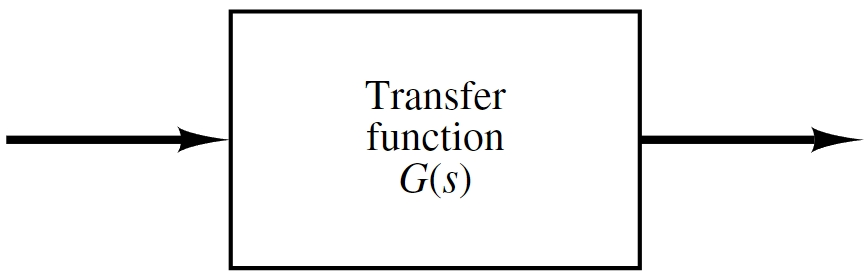
\includegraphics[width=.4\textwidth]{Chapter2/block diagram.png} %1.png是图片文件的相对路径
    \caption{Element of a block diagram} %caption是图片的标题
    \label{blockdiagram} %此处的label相当于一个图片的专属标志,目的是方便上下文的引用
\end{figure}
\begin{formal}
    Block Diagrams:框图是指对系统中每个组成部分的功能和信号流向的图形化呈现。其中的单个组成部分可以分别用block表示,其功能一般以传输函数Transfer function的形式呈现,信号流向以箭头的形式呈现,其中箭头指向block的是输入信号,箭尾指向block的为输出信号。
\end{formal}
图\ref{blockdiagram}所示为系统中任一组成部分的示意框图。其中输出信号等于输入信号乘以框图中的传输函数。由于框图的功能是用其对应部分的传输函数表示,因而其只能表现这个部分的动态特性,不能反映这个部分的实际物理结构,因此即使物理结构不同的组成部分,只要动态特性相同,就有相同的框图。
对于给定系统的整体框图的绘制形式并不唯一。
\begin{formal}
    Summing Point:图\ref{Summingpoint}所示为Summing point示意图,其十字中的"+"和"-"分别代表了信号的加减。
\end{formal}
\begin{figure}
    \centering
    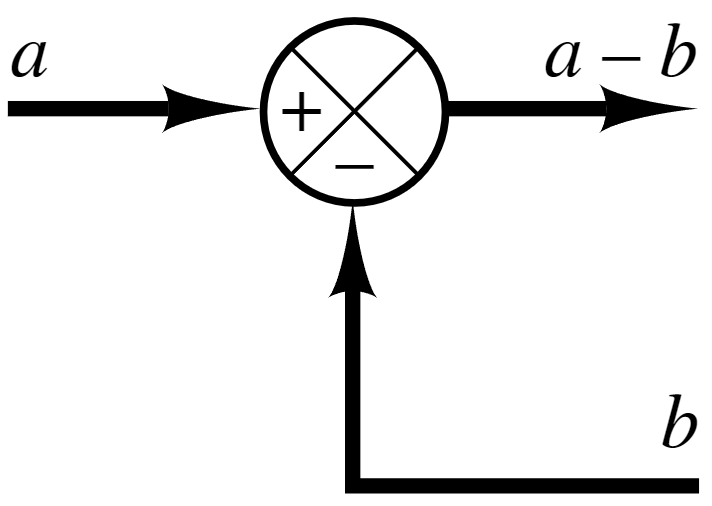
\includegraphics[width=.2\textwidth]{Chapter2/summingpoint.png} %1.png是图片文件的相对路径
    \caption{Summing point} %caption是图片的标题
    \label{Summingpoint} %此处的label相当于一个图片的专属标志,目的是方便上下文的引用
\end{figure}
\begin{formal}
    Branch Point:信号同时流向多个block或summing point的点。
\end{formal}
任何的线性系统都可以通过由blocks、summing point和branch point组成。
\begin{figure}
    \centering
    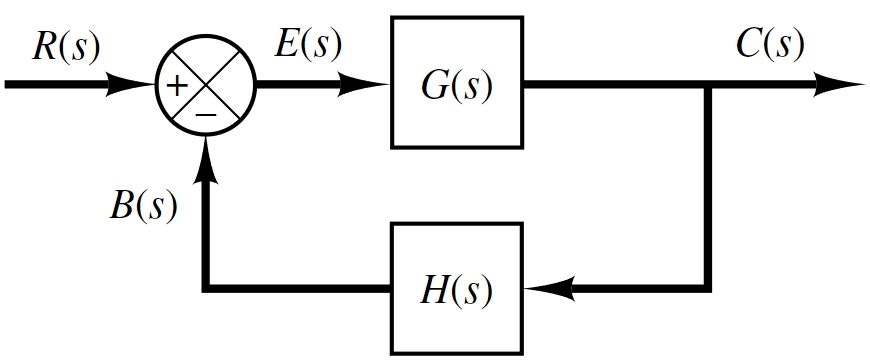
\includegraphics[width=.4\textwidth]{Chapter2/feedback system block.png} %1.png是图片文件的相对路径
    \caption{Block Diagram of a Closed-Loop System} %caption是图片的标题
    \label{BlockDiagramofaClosed-LoopSystem} %此处的label相当于一个图片的专属标志,目的是方便上下文的引用
\end{figure}
\begin{formal}
    Block Diagram of a Closed-Loop System:图\ref{BlockDiagramofaClosed-LoopSystem}所示的闭环系统框图实例,其中输出被传输回输入端与输入信号进行比较。
\end{formal}
因为要将输出信号传输回输入信号与输入信号进行比较,因此要先将输出信号的形式进行转换,转换为与输入信号相同维度(例如相同单位)的信号,再与输入信号相比较。在图\ref{BlockDiagramofaClosed-LoopSystem}中,这一转换是通过传输函数为H(s)的block实现的,其中$B(s)=H(s)C(s)$。
\begin{formal}
    Open-Loop Transfer Function:以图\ref{BlockDiagramofaClosed-LoopSystem}为例,反馈信号B(s)与actuating error信号E(s)的比值为open-loop transfer function,即$Open-loop transfer function = \frac{B(s)}{E(s)} = G(s)H(s)$
\end{formal}
\begin{formal}
    Feedforward Transfer Function:以图\ref{BlockDiagramofaClosed-LoopSystem}为例,输出信号C(s)与actuating error信号E(s)的比值为feedforward transfer function,即$Feedforward transfer function = \frac{C(s)}{E(s)} = G(s)$
\end{formal}
如果传输函数H(s)是1,则开环传输函数和前馈传输函数相同。
\begin{formal}
    Closed-Loop Transfer Function:输出信号C(s)与输入信号R(s)之间的传输函数称为 closed-loop transfer function。以图\ref{BlockDiagramofaClosed-LoopSystem}为例,输出信号C(s)与输入信号R(s)的传输函数为:
    $Closed-loop transfer function=\frac{C(s)}{R(s)}=\frac{G(s)}{1+G(s)H(s)}$
\end{formal}

\begin{formal}
    Automatic Controllers:系统中通过将输出信号的实际值与参考输入进行比较,确定输出信号相较理想值的偏离程度,进而产生能够降低这一偏离使输出信号恢复至理想值的控制信号的部分称为Automatic Controllers。其中Automatic Controller中产生控制信号的行为称为control action。
\end{formal}
以图\ref{Automaticcontroller}为例,再Automatic Controller中,先将输出与输入信号进行比较,得到比较后的信号,由于比较所得的信号较小,因而需要再通过Amplifier将其放大。除此之外,框图中Sensor的功能为将输出信号转化为与输入参考信号想同维度(一般为相同单位)的信号.
\begin{figure}
    \centering
    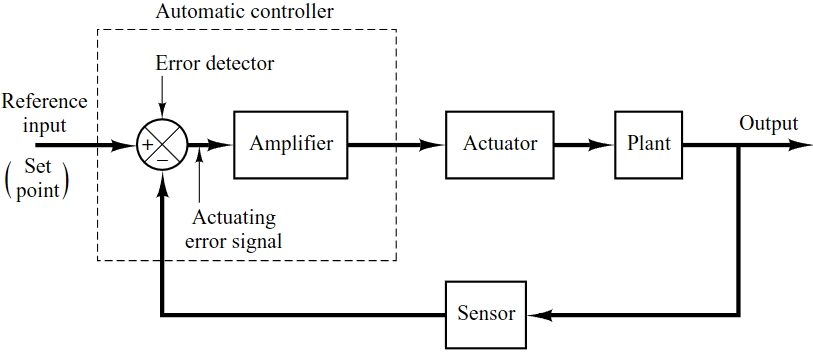
\includegraphics[width=.7\textwidth]{Chapter2/Automatic controller.png} %1.png是图片文件的相对路径
    \caption{Block diagram consists of Automatic controller} %caption是图片的标题
    \label{Automaticcontroller} %此处的label相当于一个图片的专属标志,目的是方便上下文的引用
\end{figure}

\begin{formal}
    Classifications of Industrial Controllers:
    根据Controller所采用的能源类型,可以分为:pneumatic controllers, hydraulic controllers 和 electroinic controllers。
    根据controller的具体control action,可以分为:
    \begin{enumerate}
    \item Two-position or on–off controllers
    \item Proportional controllers
    \item Integral controllers
    \item Proportional-plus-integral controllers
    \item Proportional-plus-derivative controllers
    \item Proportional-plus-integral-plus-derivative controllers
    \end{enumerate}
\end{formal}
其中每个Controller所对应的control action如下文所示:
\begin{formal}
    Two-Position or On–Off Control Action:只会产生两种固定值控制信号的控制行为。一般两种信号分别对应on和off。
    其输出信号$u(t)$与actuating error signal$e(t)$(即控制模块的输入信号,一般为反馈信号与参考输入信号的差值)的关系满足:
    \begin{equation}
        \begin{split}
        u(t)&=U_1 \qquad  for \quad e(t)>0\\
            &=U_2 \qquad  for \quad e(t)<0    
        \end{split}
    \end{equation}
    其中,$U_1$和$U_2$为常数。一般情况下,$U_1$和$U_2$要么一个为0一个非0;要么互为相反数。
\end{formal}
\begin{figure}
    \centering
    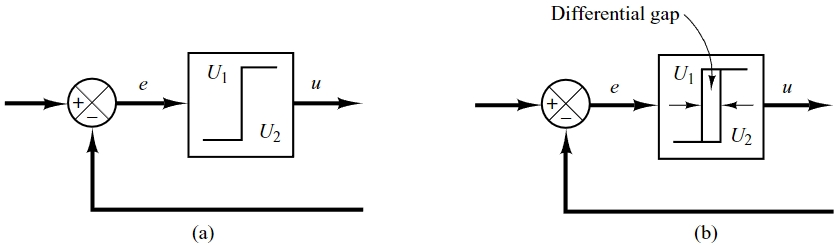
\includegraphics[width=.8\textwidth]{Chapter2/twopositioncontroller.png} %1.png是图片文件的相对路径
    \caption{Block diagram of on-off controller} %caption是图片的标题
    \label{twopositioncontroller} %此处的label相当于一个图片的专属标志,目的是方便上下文的引用
\end{figure}
图\ref{twopositioncontroller}(a)所示的是on-off controller的示意框图,这一类的controller一般由电子元件、电磁控制阀等构成。
图\ref{twopositioncontroller}(b)所示的是具有Differential gap的on-off controller示意图。

\begin{formal}
    Differential gap:输出信号发生翻转前输入信号必须经过的范围。例如迟滞窗口hysteresis window。
\end{formal}

Differential gap会迫使输出保持原值直到输入信号多变化一些,避免了可能因为信号波动导致控制器过高频的进行开关操作。
Differential gap的确定需要同时考量输出的准确度和高频开关对部件寿命的影响。

\begin{formal}
    Proportional Control Action:输出和输入信号呈比例关系,即进行比例运算的控制行为。其输入输出关系在时域中为:
    \begin{equation}
            u(t)=K_pe(t)
    \end{equation}
    拉普拉斯变换后为:
    \begin{equation}
        \frac{U(s)}{E(s)}=K_p
\end{equation}
其中$K_p$是比例增益(proportional gain)。
\end{formal}
无论实际工作机制和能源形式如何,比例控制器通常的形式为:具有合适增益的放大器。

\begin{formal}
    Integral Control Action:输出信号以与输入信号成比例的斜率进行变化的控制行为,即输出信号为输入信号的积分。其输入输出关系在时域中为:
    \begin{equation}
        \frac{du(t)}{dt}=K_ie(t)
    \end{equation}
即:
    \begin{equation}
        u(t)=K_i\int_{0}^{t}e(t)dt
    \end{equation}
其中$K_i$为可变常数。通过上述时域关系可得其传输函数transfer function为:
    \begin{equation}
        \frac{U(s)}{E(s)}=\frac{K_i}{s}
    \end{equation}
\end{formal}

\begin{formal}
    Proportional-Plus-Integral Control Action:输出信号与输入信号之间的控制行为涉及了比例运算、加法运算和积分运算的控制行为。其输入输出关系在时域中为:
    \begin{equation}
        u(t)=K_pe(t)+\frac{K_p}{T_i}\int_{0}^{t}e(t)dt
    \end{equation}
    通过上述时域关系可得其传输函数transfer function为:
    \begin{equation}
        \frac{U(s)}{E(s)}=K_p(1+\frac{1}{T_is})
    \end{equation}
    其中$T_i$称为积分时间(integral time)
\end{formal}

\begin{formal}
    Proportional-Plus-Derivative Control Action:输出信号与输入信号之间的控制行为涉及了比例运算、加法运算和微分运算的控制行为。其输入输出关系在时域中为:
    \begin{equation}
        u(t)=K_pe(t)+K_pT_d\frac{de(t)}{dt}
    \end{equation}
    通过上述时域关系可得其传输函数transfer function为:
    \begin{equation}
        \frac{U(s)}{E(s)}=K_p(1+T_ds)
    \end{equation}
    其中$T_d$称为积分时间(derivative time)
\end{formal}

\begin{formal}
    Proportional-Plus-Integral-Plus-Derivative Control Action:输出信号与输入信号之间的控制行为涉及了比例运算、加法运算、积分运算和微分运算的控制行为。其输入输出关系在时域中为:
    \begin{equation}
        u(t)=K_pe(t)+\frac{K_p}{T_i}\int_{0}^{t}e(t)dt+K_pT_d\frac{de(t)}{dt}
    \end{equation}
    通过上述时域关系可得其传输函数transfer function为:
    \begin{equation}
        \frac{U(s)}{E(s)}=K_p(1+\frac{1}{T_is}+T_ds)
    \end{equation}
\end{formal}

\begin{figure}
    \centering
    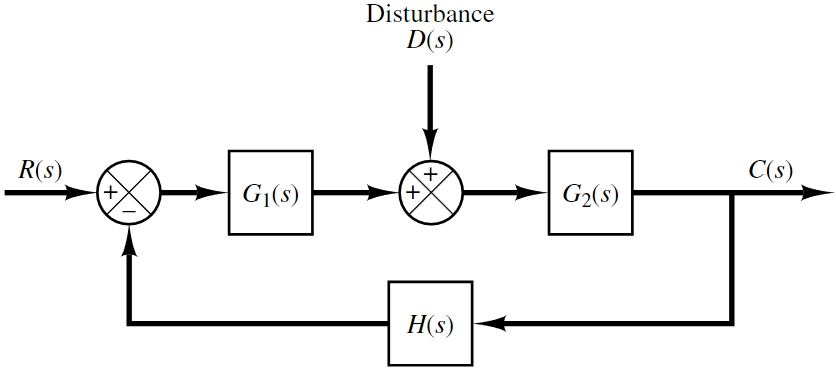
\includegraphics[width=.6\textwidth]{Chapter2/Close-loop system under disturbance.png} %1.png是图片文件的相对路径
    \caption{Closed-loop system subjected to a disturbance} %caption是图片的标题
    \label{Closed-loop system subjected to a disturbance} %此处的label相当于一个图片的专属标志,目的是方便上下文的引用
\end{figure}

\begin{formal}
    Closed-loop system subjected to a disturbance:如图\ref{Closed-loop system subjected to a disturbance}所示为受dirturbance影响的闭环系统框图,其具有两个输入,一个为R(s),一个为D(s)。
\end{formal}
根据框图\ref{Closed-loop system subjected to a disturbance}中每个模块的传输函数可知,该系统为线性时不变系统,因而总的输出响应为单个输入产生输出响应之和。
当只有$D(s)$为输入时,即$R(s)$为0时,令仅由$D(s)$产生的输出响应为$C_D(s)$,则$C_D(s)$与$D(s)$之间的关系为:
\begin{equation}
    \frac{C_D(s)}{D(s)}=\frac{G_2(s)}{1+G_1(s)G_2(s)H(s)}
\end{equation}

当只有$R(s)$为输入时,即$D(s)$为0时,令仅由$R(s)$产生的输出响应为$C_R(s)$,则$C_R(s)$与$R(s)$之间的关系为:
\begin{equation}
    \frac{C_R(s)}{R(s)}=\frac{G_1(s)G_2(s)}{1+G_1(s)G_2(s)H(s)}
\end{equation}

通过将两个输入单独作用时的输出响应进行求和,可以得到两个输入同时作用下的输出响应(叠加定理),即:
\begin{equation}
    \begin{split}
        C(s)&=C_R(s)+C_D(s)\\
        &=\frac{G_2(s)}{1+G_1(s)G_2(s)H(s)}[G_1(s)R(s)+D(s)]
    \end{split}
\end{equation}

当$|G_1(s)H(s)|>>1$时,传输函数$\frac{C_D(s)}{D(s)}$几乎为0,即dirturbance对输出响应基本不造成影响,实现了对disturbance的抑制。
当$|G_1(s)G_2(s)H(s)|>>1$时,传输函数$\frac{C_R(s)}{R(s)}≈\frac{1}{H(s)}$,意味着输入信号产生的输出响应受$G_1(s)$和$G_2(s)$的影响越来越小,将只受$H(s)$影响,这种情况下,如果$H(s)=1$,则输入和输出相等。

\begin{formal}
    Procedures for Drawing a Block Diagram:
    \begin{enumerate}
        \item 得到描述系统动态特性的方程;
        \item 在假定初始条件为0的情况下,对方程进行拉普拉斯变换;
        \item 对每个拉普拉斯形式下的方程用blocks、summing point和branch进行表示;
        \item 对所有的拉普拉斯方程各自对应的框图进行组合。
    \end{enumerate}
\end{formal}
其中只有当后一级的block不会对前一级的block造成影响时才可以进行两个block间的串联。如果后一级的block会对前一级的block造成影响,则需要将这两个block整合为一个整体的block。
任何非负载组件(什么是nonloading components?)对应框图的级联都可以被一个单独的block所取代,只是这个取代的block的传输函数为级联的每个block的传输函数的乘积。
尽管框图可以通过上述方式进行简化,但简化后的框图中的传输函数的形式会变得更加复杂。

\begin{formal}
    Simplication of Block Diagrams:
    \begin{enumerate}
        \item 将互相耦合的反馈环路解耦。
        \item 依次将最小反馈环路、次小反馈环路...用一个单独的block进行取代,这个block的传输函数由反馈环路中各个模块的传输函数决定。
        \item 得到化简后的Block Dirgram。
    \end{enumerate}
\end{formal}

\begin{figure}
    \centering
    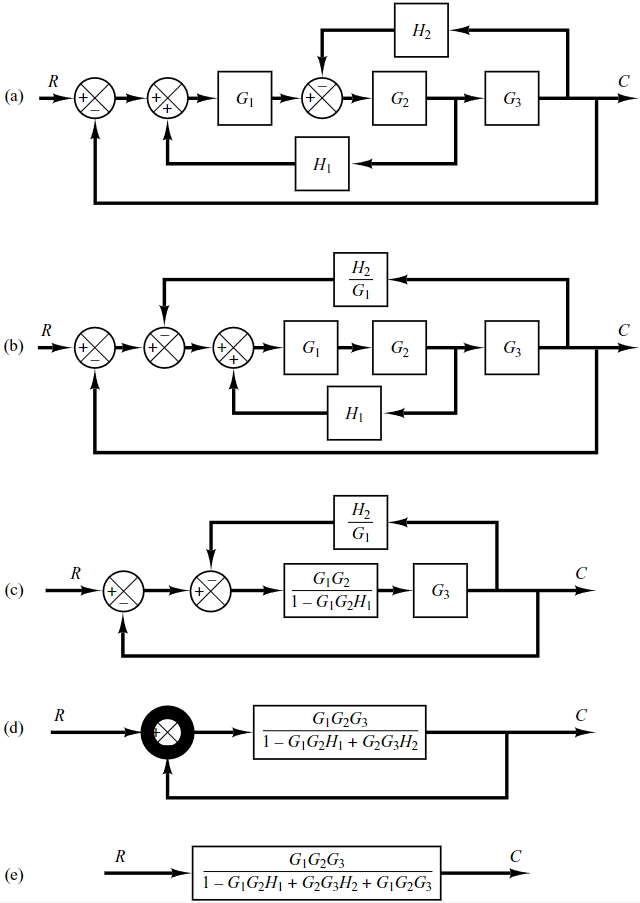
\includegraphics[width=.6\textwidth]{Chapter2/simplificationofbd.png} %1.png是图片文件的相对路径
    \caption{Simplication of Block Diagrams} %caption是图片的标题
    \label{Simplication of Block Diagrams} %此处的label相当于一个图片的专属标志,目的是方便上下文的引用
\end{figure}

图\ref{Simplication of Block Diagrams}所示为框图化简的示例。
从最终化简所得的传输函数可知,闭环传输函数$C(s)/R(s)$的分子为前馈路径中传输函数的乘积$G_1G_2G_3$,分母为:

\begin{equation}
    \begin{split}
        &1+\sum ({product\_of\_the\_transfer\_functiuons\_around\_each\_loop})\\
        =&1+(-G_1G_2H_1+G_2G_3H_2+G_1G_2G_3)\\
        =&1-G_1G_2H_1+G_2G_3H_2+G_1G_2G_3
    \end{split}
\end{equation}

其中正反馈产生的是负乘积项,负反馈产生的是正乘积项。

\subsection{State Space建模的概念及其原理}

\begin{formal}
    Modern Control Theory:现代控制理论是基于concept of state而建立的,用于分析和设计复杂控制系统的方法。复杂控制系统:具有多个输入、多个输出并且可能是时变的系统。
\end{formal}

相较于只能应用于“单输入单输出的线性时不变系统”的Conventional Control Theory,Modern Control Theory可以适用于“多输出多输出”、“线性或非线性”、“时变或非时变”的几乎所有系统。

造成这一影响的主要原因是,Conventional Control Theory所基于的是复频域分析,即对原本时域的关系进行拉普拉斯变换后再分析,这一分析过程只有LTI系统适用;Modern Control Theory所基于的是时域分析方法,是对最本质的时域微分方程组分析,因此无论系统是何种类型均适用。

此外,根据上述分析可知,如果系统是LTI系统,则其将同时适用于Conventional Control Theory和Modern Control Theory。

\begin{formal}
    State:是指最小的一组变量,这组变量需要满足:当明确其在$t=t_0$时刻的值和$t≥t_0$时刻的输入后,可以完全确定在$t≥t_0$后任意时刻的系统行为。
\end{formal}

\begin{formal}
    State Variables:State所对应的那一组变量中的变量称为State Variables。
\end{formal}

同一系统可以选用不同的State Variables,但所用的State Variables的数量是相同的。

\begin{formal}
    State Vector:如果State中包含n个State Variables,则由这n个State Variables所构成的向量称为State Vector。
\end{formal}

\begin{formal}
    State Space:由State中所有的State Variables作为坐标轴所组成的空间称为State Space。任何的状态都可以表示在这个状态空间中。
\end{formal}

在state-space分析中进行数学建模时,需要考虑的有三种变量:1.input variables;2.output variables;3.state variables。其中对于state variables而言:

The dynamic system must involve elements that memorize the values of the input for
$t ≥ t_1$ . Since integrators in a continuous-time control system serve as memory devices,
the outputs of such integrators can be considered as the variables that define the internal state of the dynamic system.Thus the outputs of integrators serve as state variables.
The number of state variables to completely define the dynamics of the system is equal
to the number of integrators involved in the system.(系统的状态变量数$\Longleftrightarrow$ 系统中所采用的积分器的数量$\Longleftrightarrow$时域微分方程中输出的介数)

假定一个具有r个输入m个输出的系统包含n个积分器,即输入、输出、状态变量的数量依次为r、m、n。令r个输入分别为:$u_1(t)、u_2(t)...u_r(t)$;m个输入分别为:$y_1(t)、y_2(t)...y_m(t)$;定义每个积分器的输出为状态变量:$x_1(t)、x_2(t)...x_n(t)$,则每个积分器的输入相应为:$x_1^{(1)}(t)、x_2^{(1)}(t)...x_n^{(1)}(t)$。

则这个系统的状态变量可以描述为(虽然是三个量y,u,x,但只有两个量之间是互相独立的,即只要有两个量确定,第三个量就确定了:例如系统的输入和输出确定后,其内部的状态一定是确定的;或是输入和状态确定后,其输出也一定是确定的。因此输出的函数y可以通过x和u以及t为变量进行描述;同理积分器的输入$x_n^{(1)}(t)$可以通过在y,u,x中任取两个量,再加上t进行描述):

\begin{equation}
    \begin{split}
        &x_1^{(1)}(t)=f_1(x_1,x_2,...,x_n;u_1,u_2,...,u_r;t)\\
        &x_2^{(1)}(t)=f_2(x_1,x_2,...,x_n;u_1,u_2,...,u_r;t)\\
        &...\\
        &x_n^{(1)}(t)=f_n(x_1,x_2,...,x_n;u_1,u_2,...,u_r;t)
    \end{split}
\end{equation}

这个系统的输出变量可以描述为:
\begin{equation}
    \begin{split}
        &y_1(t)=g_1(x_1,x_2,...,x_n;u_1,u_2,...,u_r;t)\\
        &y_2(t)=g_2(x_1,x_2,...,x_n;u_1,u_2,...,u_r;t)\\
        &...\\
        &y_m(t)=g_n(x_1,x_2,...,x_n;u_1,u_2,...,u_r;t)
    \end{split}
\end{equation}

当按照下式进行定义后:

\begin{equation}
    \begin{split}
        &x(t)=
        \begin{bmatrix}
            x_1(t)\\
            x_2(t)\\
            ...\\
            x_n(t)
        \end{bmatrix}
        \quad
        f(x,u,t)=
        \begin{bmatrix}
            f_1(x_1,x_2,...,x_n;u_1,u_2,...,u_r;t)\\
            f_2(x_1,x_2,...,x_n;u_1,u_2,...,u_r;t)\\
            ...\\
            f_n(x_1,x_2,...,x_n;u_1,u_2,...,u_r;t)
        \end{bmatrix}\\
        &y(t)=
        \begin{bmatrix}
            y_1(t)\\
            y_2(t)\\
            ...\\
            y_m(t)
        \end{bmatrix}
        \quad
        g(x,u,t)=
        \begin{bmatrix}
            g_1(x_1,x_2,...,x_n;u_1,u_2,...,u_r;t)\\
            g_2(x_1,x_2,...,x_n;u_1,u_2,...,u_r;t)\\
            ...\\
            g_m(x_1,x_2,...,x_n;u_1,u_2,...,u_r;t)
        \end{bmatrix}
        \quad
        u(t)=
        \begin{bmatrix}
            u_1(t)\\
            u_2(t)\\
            ...\\
            u_r(t)
        \end{bmatrix}
    \end{split}
\end{equation}

可得:
\begin{equation}
    x^{(1)}(t)=f(x,u,t)\label{state equation}
\end{equation}
\begin{equation}
    y(t)=g(x,u,t)\label{output equation}
\end{equation}

其中Eq.(\ref{state equation})称为state equation,Eq.(\ref{output equation})称为output equation。其中如果f或g是时间的函数,则这个系统是时变系统。

如果Eq.(\ref{state equation})和Eq.(\ref{output equation})在工作点附近满足线性性(即满足叠加定理),则state equation和output equation可以表示为:
\begin{equation}
    x^{(1)}(t)=A(t)x(t)+B(t)u(t)
\end{equation}
\begin{equation}
    y(t)=C(t)x(t)+D(t)u(t)
\end{equation}

其中$A(t)$称为state matrix,$B(t)$称为input matrix,$C(t)$称为output matrix,$D(t)$称为direct transmission matrix。

如果f或g是不是时间的函数,则这个系统是时不变系统,且Eq.(\ref{state equation})和Eq.(\ref{output equation})在工作点附近满足线性性时,则state equation和output equation可以表示为:
\begin{equation}
    x^{(1)}(t)=Ax(t)+Bu(t)\label{seLTI}
\end{equation}
\begin{equation}
    y(t)=Cx(t)+Du(t)\label{oeLTI}
\end{equation}

其中Eq.(\ref{seLTI})和Eq.(\ref{oeLTI})分别是LTI系统的state equation和output equation。

由于LTI系统的动态特性既可以通过state equation和output equation的组合表示,也可以通过系统的传输函数表示。那么对于LTI系统而言这两者的关联为:

\begin{formal}
    Correlation Between Transfer Functions and State-Space Equations:
\end{formal}

由于系统为LTI系统,因此这个系统的动态特性可以通过Eq.(\ref{seLTI})和Eq.(\ref{oeLTI})进行描述。用$Y(s)、U(s)、X(s)$分别表示$y(t)、u(t)和x(t)$的拉普拉斯变换,因此可得:

\begin{equation}
    sX(s)-x(0)=AX(s)+BU(s)
\end{equation}
\begin{equation}
    Y(s)=CX(s)+DU(s)
\end{equation}

如果要通过确定所施加输入信号与输出信号之间的关系得到系统的传输函数,则初始条件需设为0,因此可得:
\begin{equation}
    \begin{split}
        &sX(s)=AX(s)+BU(s)\\
        or \quad &(sI-A)X(s)=BU(s)\\
        or \quad &X(s)=(sI-A)^{-1}BU(s)
    \end{split}
\end{equation}

其中I为单位矩阵,通过将上式代入可得:
\begin{equation}
    \begin{split}
        &Y(s)=[C(sI-A)^{-1}B+D]U(s)\\
        or \quad &\frac{Y(s)}{U(s)}=C(sI-A)^{-1}B+D
    \end{split}
\end{equation}

考虑到当初始条件为0时,LTI系统的传输函数为$G(s)=\frac{Y(s)}{U(s)}$,因此可得:

\begin{equation}
    G(s)=\frac{Y(s)}{U(s)}=C(sI-A)^{-1}B+D
\end{equation}

如果系统是单输入单输出系统,则上式G(s)所表示的时系统的传输函数transfer function;如果是多输入多输出系统,则上式G(s)所表示的时系统的传输矩阵transfer matrix。如果有r个输入(输入为r维),有m个输出(输出为m维),则传输矩阵G(s)是一个$m×r$ 的矩阵。

\subsection{微分方程的State-Space建模}

\begin{formal}
    State-Space Representation of nth-Order Systems of Linear Differential Equations in which the Forcing Function Does Not Involve Derivative Terms.(输入没有求导项的线性微分方程)
\end{formal}

假定这类微分方程是n阶级微分方程,则其必然满足下式:
\begin{equation}
    y^{(n)}+a_1y^{(n-1)}+...+a_{n-1}y^{(1)}+a_ny=u\label{eqffndt}
\end{equation}

由于只要确定$y(0),y^{(1)}(0),...,y^{(n-1)}(0)$和$t≥0$时刻的输入,就可以确定future behavior of the system,因此选用$y(t),y^{(1)}(t),...,y^{(n-1)}(t)$作为一组状态变量(?)。故而将状态变量定义为:
\begin{equation}
    \begin{split}
        x_1&=y\\
        x_2&=y^{(1)}\\
        &...\\
        x_n&=y^{(n-1)}
    \end{split}
\end{equation}

因此可得:
\begin{equation}
    \begin{split}
        x^{(1)}_1&=x_2\\
        x^{(1)}_2&=x_3\\
        &...\\
        x^{(1)}_{n-1}&=x_n\\
        x^{(1)}_{n}&=y^{(n)}=-a_nx_1-...-a_1x_n+u
    \end{split}
\end{equation}
令:
\begin{equation}
    x=
    \begin{bmatrix}
        x_1\\
        x_2\\
        .\\
        .\\
        .\\
        x_n
    \end{bmatrix}
    \quad
    A=
    \begin{bmatrix}
        0&1&0&...&0\\
        0&0&1&...&0\\
        .&.&.& &.\\
        .&.&.& &.\\
        .&.&.& &.\\
        0&0&0&...&1\\
        -a_n&-a_{n-1}&-a_{n-2}&...&-a_1\\
    \end{bmatrix}
    \quad
    B=
    \begin{bmatrix}
        0\\
        0\\
        .\\
        .\\
        .\\
        0\\
        1\\
    \end{bmatrix}
\end{equation}

则可得:
\begin{equation}
    x^{(1)}=Ax+Bu
\end{equation}

又因为:
\begin{equation}
    y=
    \begin{bmatrix}
        1&0&0&.&.&.&0
    \end{bmatrix}
    \begin{bmatrix}
        x_1\\
        x_2\\
        .\\
        .\\
        .\\
        x_n\\
    \end{bmatrix}
\end{equation}

所以可得:
\begin{equation}
    \begin{split}
        y&=Cx\\
        where \quad C&=
        \begin{bmatrix}
            1&0&0&.&.&.&0
        \end{bmatrix}
    \end{split}
\end{equation}

综上所示,输入无求导项的微分方程的state equation为$x^{(1)}=Ax+Bu$,output equation为$y=Cx$。


\begin{formal}
    State-Space Representation of nth-Order Systems of Linear Differential Equations in which the Forcing Function Involves Derivative Terms.(输入有求导项的线性微分方程)
\end{formal}

假定这类微分方程是n阶级微分方程,则其必然满足下式:
\begin{equation}
    y^{(n)}+a_1y^{(n-1)}+...+a_{n-1}y^{(1)}+a_ny=b_0u^{(n)}+b_1u^{(n-1)}+...+b_{n-1}u^{(1)}+b_nu
\end{equation}

对于这类微分方程,一种可取得状态变量定义方法为:
\begin{equation}
    \begin{split}
        &x_1=y-\beta_0u\\
        &x_2=y^{(1)}-\beta_0u^{(1)}-\beta_1u=x^{(1)}_1-\beta_1u\\
        &x_3=y^{(2)}-\beta_0u^{(2)}-\beta_1u^{(1)}-\beta_2u=x^{(2)}_1-\beta_2u\\
        &.\\
        &.\\
        &.\\
        &x_n=y^{(n-1)}-\beta_0u^{(n-1)}-\beta_1u^{(n-2)}-...-\beta_{n-2}u^{(1)}-\beta_{n-1}u=x^{(1)}_{n-1}-\beta_{n-1}u
    \end{split}
\end{equation}

其中$\beta_0,\beta_1,\beta_2,...,\beta_{n-1}$为:
\begin{equation}
    \begin{split}
        &\beta_0=b_0\\
        &\beta_1=b_1-a_1\beta_0\\
        &\beta_2=b_2-a_1\beta_1-a_2\beta_0\\
        &\beta_3=b_3-a_1\beta_2-a_2\beta_1-a_3\beta_0\\
        &.\\
        &.\\
        &.\\
        &\beta_{n-1}=b_{n-1}-a_1\beta_{n-2}-...-a_{n-2}\beta_1-a_{n-1}\beta_0
    \end{split}
\end{equation}

因此可得:
\begin{equation}
    \begin{split}
        &x_1^{(1)}=x_2+\beta_1u\\
        &x_2^{(1)}=x_3+\beta_2u\\
        &.\\
        &.\\
        &.\\
        &x_{n-1}^{(1)}=x_{n}+\beta_{n-1}u\\
        &x_n^{(1)}=-a_nx_1-a_{n-1}x_2-...-a_1x_n-\beta_nu\\
        where \quad &\beta_n=b_n-a_1\beta_{n-1}-...-a_{n-1}\beta_1-a_{n-1}\beta_0
    \end{split}
\end{equation}

即:
\begin{equation}
    \begin{split}
        \begin{bmatrix}
            x^{(1)}_1\\
            x^{(1)}_2\\
            .\\
            .\\
            .\\
            x^{(1)}_{n-1}\\
            x^{(1)}_m\\
        \end{bmatrix}
        &=
        \begin{bmatrix}
            0&1&0&...&0\\
            0&0&1&...&0\\
            .&.&.& &.\\
            .&.&.& &.\\
            .&.&.& &.\\
            0&0&0&...&1\\
            -a_n&-a_{n-1}&-a_{n-2}&...&-a_1\\
        \end{bmatrix}
        \begin{bmatrix}
            x_1\\
            x_2\\
            .\\
            .\\
            .\\
            x_{n-1}\\
            x_n\\
        \end{bmatrix}
        +
        \begin{bmatrix}
            \beta_1\\
            \beta_2\\
            .\\
            .\\
            .\\
            \beta_{n-1}\\
            \beta_n\\
        \end{bmatrix}
        u\\
        y&=    
        \begin{bmatrix}
            1&0&0&.&.&.&0
        \end{bmatrix}
        \begin{bmatrix}
            x_1\\
            x_2\\
            .\\
            .\\
            .\\
            x_n\\
        \end{bmatrix}
        +
        \beta_0u
    \end{split}
\end{equation}

根据$x^{(1)}=Ax+Bu$和$y(t)=Cx+Du$可知A、B、C和D分别为:
\begin{equation}
    A=
    \begin{bmatrix}
        0&1&0&...&0\\
        0&0&1&...&0\\
        .&.&.& &.\\
        .&.&.& &.\\
        .&.&.& &.\\
        0&0&0&...&1\\
        -a_n&-a_{n-1}&-a_{n-2}&...&-a_1\\
    \end{bmatrix};
    \quad
    B=
    \begin{bmatrix}
        \beta_1\\
        \beta_2\\
        .\\
        .\\
        .\\
        \beta_{n-1}\\
        \beta_n\\
    \end{bmatrix};
    \quad
    C=
    \begin{bmatrix}
        1&0&0&.&.&.&0
    \end{bmatrix};
    \quad
    D=\beta_0=b_0
\end{equation}

\subsection{非线性数学模型线性化}
根据Tylor Series可知,一个函数$f(x)$上某一点$(x_0,y_0)$附近的值可以通过一系列多项式求和得到,即:
\begin{equation}
    \begin{split}
        y&=f(x)\\
        &=f(x_0)+\frac{df}{dx}(x-x_0)+\frac{1}{2!}\frac{d^2f}{dx^2}(x-x_0)^2+...
    \end{split}
\end{equation}

其中$\frac{df}{dx}、\frac{d^2f}{dx^2}...$等项取$x=x_0$处的值。

根据Tlyor展开式可以看出,当x非常接近$x_0$时,$y≈f(x_0)+\frac{df}{dx}(x-x_0)$,即在这一点附近非常小的范围内,非线性函数可以用一个线性函数等效近似,因而原本非线性的系统就可以用一个线性系统进行等效分析计算。

然而这一近似方法仅适用于,在某一工作点附近微小波动的系统,如果波动幅度过大,高阶项不再可忽略,如果继续用上述的等效线性模型分析,将会导致非常严重的误差。

放大电路是这一近似方法非常好的应用对象,尽管放大电路这个系统是一个由非线性函数所描述的系统,但由于其是围绕某一工作点附近进行微小波动,因此如果把$Vin=VIN+vin$和$Vout=VOUT+vout$分别看作输入和输出,其中$VIN$和$VOUT$为工作点,且之间满足的函数关系为$Vout=f(Vin)$,则可以得到:
\begin{equation}
    \begin{split}
        Vout&≈f(VIN)+\frac{df}{dVin}(Vin-VIN)\\
        &≈VOUT+\frac{df}{dVin}vin
    \end{split}
\end{equation}

即:$vout=Vout-VOUT=\frac{df}{dVin}vin$。

即:$Av=\frac{vout}{vin}=\frac{df}{dVin}$=输入输出曲线在工作点处的斜率。

也因此对于放大器的输入信号而言,如果放大器的线性性较差,那么只有非常小范围的输入信号会被较好的“线性放大”(近似的),超出这个范围外的输入信号就会被原本泰勒展开中的非线性项所影响,导致输出信号相对于输入信号失真;如果放大器的线性性较好,那么就有更宽的输入范围可以实现“线性放大”,可以实现对更多的信号进行“不失真”的放大传输。

从增益表达式的推到上也可以看出,通过求曲线在工作点处的斜率求得信号增益的方法实际也只适用于幅度极小的输入信号,否则这一方法所求得的增益将于实际增益有较大偏差。

当系统有多个输入时,泰勒展开找到近似线性方程从而实现非线性系统线性化的方法也是适用的。若系统满足的方程为$y=f(x_1,x_2)$,通过泰勒展开可得函数在工作点$(x_{10},x_{20})$附近的表达式为:
\begin{equation}
    \begin{split}
        y=&f(x_{10},x_{20})+[\frac{\partial f}{\partial x_1}(x_1-x_{10})+\frac{\partial f}{\partial x_2}(x_2-x_{20})]+...
    \end{split}
\end{equation}
其中$\frac{\partial f}{\partial x_1}、\frac{\partial f}{\partial x_2}...$等项取$(x_{10},x_{20})$处的值。

同理,当波动较小时,忽略高阶项可得线性方程:
\begin{equation}
    y=f(x_{10},x_{20})+[\frac{\partial f}{\partial x_1}(x_1-x_{10})+\frac{\partial f}{\partial x_2}(x_2-x_{20})]
\end{equation}

因此对于多输入系统,通过泰勒展开围绕工作点附近进行线性化的方法也是适用的。

\newpage

\section{力学系统和电子系统的数学模型}
\subsection{Introduction}
\begin{formal}
    力学系统:以牛顿第二定律为基本运算法则。
\end{formal}

\begin{formal}
    电子电路:以Kirchhoff's laws为基本运算法则。
\end{formal}
    通过每种系统的最基本的法则可以推导出每种系统的数学模型。

\subsection{力学系统数学建模}

\subsection{电子系统数学建模}
\begin{formal}
    基尔霍夫电流定律:电路中任一节点处流入的电流之和等于流出的电流之和。
\end{formal}

\begin{formal}
    基尔霍夫电压定律:电路中任意环路中的所有元件的压降的代数和为0。
\end{formal}

通过应用KCL、KVL就可以得到电子电路的数学模型。

\begin{formal}
    LRC电路:由电感、电阻、电容所组成的电路称为LRC电路。
\end{formal}

\begin{formal}
    电阻、电感、电容元件的电流电压关系:
    \begin{itemize}
        \item 电阻R:$R=\frac{U_{ab}}{I_{ab}}$
        \item 电感L:$U_{ab}=L*\frac{d(I_{ab})}{dt}$
        \item 电容C:$I_{ab}=C*\frac{d(U_{ab})}{dt}$
    \end{itemize}
    由上述关系可知,无论是电阻、电感还是电容,其电流电压关系总是$U_{ab}$与$I_{ab}$的关系。其中$U_{ab}=U_{a}-U_{b}$为节点a和节点b的电压差;$I_{ab}$为从节点a流向节点b的电流。
\end{formal}

\begin{figure}
    \centering
    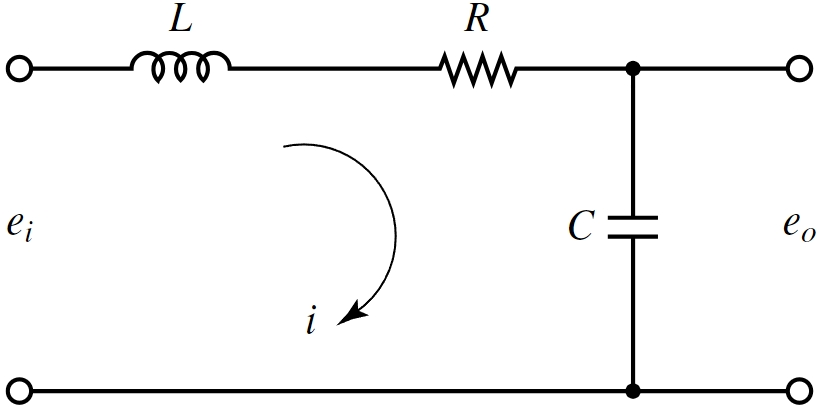
\includegraphics[width=.4\textwidth]{Chapter3/LRCcircuit.png} %1.png是图片文件的相对路径
    \caption{LRC circuit} %caption是图片的标题
    \label{LRCcircuit} %此处的label相当于一个图片的专属标志,目的是方便上下文的引用
\end{figure}

以图\ref{LRCcircuit}所示LRC电路为例,根据基尔霍夫电压定律可得:

\begin{equation}
    L\frac{di(t)}{dt}+Ri(t)+\frac{1}{C}\int_{0_-}^{t}{i(\tau)d\tau}=e_i(t)
\end{equation}

\begin{equation}
    \frac{1}{C}\int_{0_-}^{t}{i(\tau)d\tau}=e_o(t)
\end{equation}

该LRC电路的传输函数:

当初始条件为0时,根据拉普拉斯的微积分特性可得:
\begin{equation}
    \begin{split}
        LsI(S)+RI(s)+\frac{1}{C}\frac{1}{s}I(s)&=E_i(s) \\
        \frac{1}{C}\frac{1}{s}I(s)&=E_o(s)
    \end{split}
\end{equation}

因此可得LRC电路的传输函数为:
\begin{equation}
    \frac{E_o(s)}{E_i(s)}=\frac{1}{LCs^2+RCs+1}
\end{equation}

该LRC电路的状态空间方程:

根据LRC电路的时域微分方程可得输入输出所满足的时域微分方程为:
\begin{equation}
    e^{(2)}_o(t)+\frac{R}{L}e^{(1)}_o(t)+\frac{1}{LC}e_o(t)=\frac{1}{LC}e_i(t)
\end{equation}

通过上述时域方程可知为二阶微分方程,因此需要设置两个状态变量:
\begin{equation}
    \begin{split}
        x_1(t)&=e_o(t)\\
        x_2(t)&=e^{(1)}_o(t)
    \end{split}
\end{equation}

为与第二章中所推导的状态空间方程形式相同,因此用$u$表示$e_i$,用$y$表示$e_o$,因此可得:

\begin{equation}
    \begin{bmatrix}
        x^{(1)}_1\\
        x^{(1)}_2
    \end{bmatrix}
    =
    \begin{bmatrix}
        0&1\\
        -\frac{1}{LC}&-\frac{R}{L}
    \end{bmatrix}
    \begin{bmatrix}
        x_1\\
        x_2
    \end{bmatrix}
    +
    \begin{bmatrix}
        0\\
        \frac{1}{LC}
    \end{bmatrix}
    u
\end{equation}
\begin{equation}
    y=
    \begin{bmatrix}
        1&0
    \end{bmatrix}
    \begin{bmatrix}
        x_1\\
        x_2
    \end{bmatrix}
\end{equation}

上示两式即分别为该LRC电路的state equation和output equation。

\begin{formal}
    多级联元件电路的传输函数
\end{formal}

\begin{figure}
    \centering
    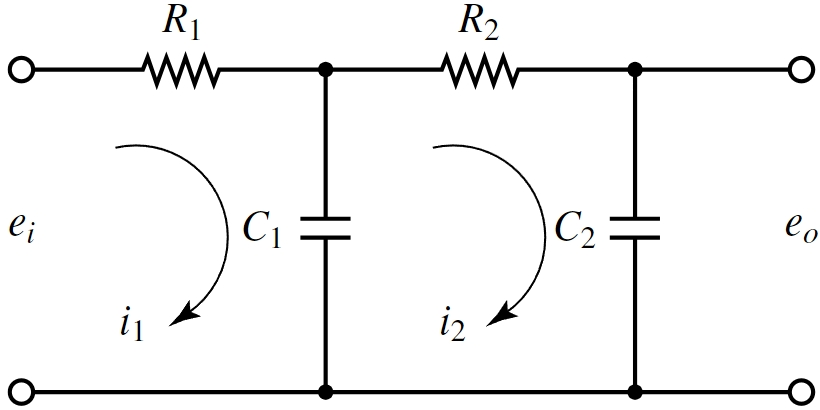
\includegraphics[width=.4\textwidth]{Chapter3/cascadecircuit.png} %1.png是图片文件的相对路径
    \caption{Circuit of Cascaded Elements} %caption是图片的标题
    \label{cascadecircuit} %此处的label相当于一个图片的专属标志,目的是方便上下文的引用
\end{figure}

以图\ref{cascadecircuit}所示的多级联元件电路为例。从电路图中可以明显的发现第二级电路(R2C2部分)对第一级电路(R1C1部分)会产生负载效应(Loading effect)。

\begin{formal}
    Loading effect:当后一级系统会对前一级系统产生影响时,则称第二级系统会对第一级产生负载效应。具体为:不存在第二级系统时的第一级的输出与存在第二级系统时的第一级的输出情况不同,即第一级的输出函数因为第二级的出现而改变。
\end{formal}

\begin{formal}
    Nonloading effect:当后一级系统不会对前一级系统产生影响时,则称第二级系统不会对第一级产生负载效应,即非负载效应。具体为:不存在第二级系统时的第一级的输出与存在第二级系统时的第一级的输出情况完全相同。如果第二级会产生影响但影响非常小可以忽略不计,此时也可以近似看作nonloading effect。
\end{formal}

因此只有两级电路之间互相不存在负载效应时,两级电路中的每一级可以分别看作一个系统,级联后系统总的传输函数等于两个单级电路系统的传输函数的乘积。若存在负载效应,就必须将这两级电路看作一个系统,并对这个系统进行专门的传输函数计算。

造成这一现象的本质原因是,在推导单极电路的传输函数时,我们假定了输出端不存在负载效应。因此这时推导出的传输函数,只在这个电路所在系统的后级不会对其产生负载效应时,才成立;而如果后级会对其产生负载效应,则我们推导的单极电路的传输函数就不再成立。

在组合电路之中,通常会选择在进行组合的两级电路之间加入一个放大器,从而消除负载效应。也就是说这个放大器不会对第一级产生负载效应,同时第二级也不会对这个放大器产生负载效应。

根据基尔霍夫定律以及基本元件的伏安特性可得描述该电路的方程:
\begin{equation}
    \frac{1}{C_1}\int_{0_-}^{t}(i_1(\tau)-i_2(\tau))d\tau+R_1i_1(t)=e_i(t)
\end{equation}
\begin{equation}
    \frac{1}{C_1}\int_{0_-}^{t}(i_2(\tau)-i_1(\tau))d\tau+R_2i_2(t)+\frac{1}{C_2}\int_{0_-}^{t}i_2(\tau)d\tau=0
\end{equation}
\begin{equation}
    \frac{1}{C_2}\int_{0_-}^{t}i_2(\tau)d\tau=e_o(t)
\end{equation}

假定初始条件为0,对上述方程进行拉普拉斯变换可得:
\begin{equation}
    \frac{1}{C_1s}[I_1(s)-I_2(s)]+R_1I_1(s)=E_i(s)
\end{equation}
\begin{equation}
    \frac{1}{C_1s}[I_2(s)-I_1(s)]+R_2I_2(s)+\frac{1}{C_2s}I_2(s)=0
\end{equation}
\begin{equation}
    \frac{1}{C_2s}I_2(s)=E_o(s)
\end{equation}

对上述方程进行整理可得系统的传输函数为:
\begin{equation}
    \begin{split}
        \frac{E_o(s)}{E_i(s)}&=\frac{1}{(R_1C_1s+1)(R_2C_2s+1)+R_1C_2s}\\
        &=\frac{1}{R_1C_1R_2C_2s^2+(R_1C_1+R_2C_2+R_1C_2)s+1}
    \end{split}
\end{equation}

\begin{formal}
    复阻抗:如果某一元件两端的电压和电流的拉普拉斯变换分别为$U(s)$和$I(s)$,并满足关系$U(s)/I(s)=Z(s)$,则我们可以将其看作阻抗为$Z(s)$的电阻进行计算从而求得传输函数。
    
    当初始条件为零时,电阻、电容、电感的复阻抗为:
    \begin{itemize}
        \item 电阻:复阻抗为$R$。
        \item 电容:复阻抗为$1/sC$
        \item 电感:复阻抗为$Ls$
    \end{itemize}
\end{formal}

这一方法并不仅限于拉普拉斯域中适用,实际上所有情况下均使用。以下将对这一方法的原理本质和适用范围进行分析:

对于任意一个由任意器件所组成的电路,我们所关心的实际只有这个电路的电压特性和电流特性,而这两个特性是由组成电路的各个元件的伏安特性所决定,也就是说,只要电路中元件的伏安特性相同,那无论元件是什么,都会求得相同的电压和电流特性。这是因为,求解电流电压特性的本质其实是求解由每个元件所满足的伏安特性的方程所组成的方程组,只要方程组里的方程一样,那求得的电路特性一定是一样的。

因此如果有一个元件的伏安特性为$U_{ab}/I_{ab}=R_{ab}$,那我们就可以用和它具有相同伏安特性的元件对它进行替代,并通过替代后的电路求得和原电路相同的结果。对于具有这个伏安特性的元件而言,阻值为$R_{ab}$的电阻元件就具备与其完全相同的伏安特性,因此可以在电路中将原本的元件用电阻$R_{ab}$进行替换,并求得和原电路相同的结果,即相同的电流电压特性。

用具有相同伏安特性的电阻元件去取代原本的电路元件的本质原因是,对于电阻而言我们具有更熟练的分析计算能力,例如对于并联电阻有总电阻的计算公式为:$R=\frac{R1R2}{R1+R2}$,对于串联电阻有总计算公式为:$R=R1+R2$。如果用电阻等价替代原元件,我们能更快更直观的对电路有所判断分析和计算。当然如果我们不用电阻等效替代这个元件进行电路分析也是可以的,不过在对这个元件进行最基本的运算后会发现,所求得的结果和用电阻替代并采用电阻的公式计算所得的结果完全一致。

要注意的一点是,串并联电阻的计算公式只适用于满足关系为“$U_{ab}/I_{ab}=R_{ab}$”并且满足串并联所对应的方程的情况,毕竟串并联电阻的计算公式的推导是基于上述方程的。

除了上述的对于具备“两端点的电压以及这两个端点之间电流关系”的元件,可以用电阻元件进行等价替代,对于“电压所对应的两个端点和电流所对应的两个端点不同”的元件,同样可以通过一个具备相同伏安特性的元件进行等价替代,这个元件就是压控电流源,其原理与上述电阻一致。

综上所述,对于满足“$U_{ab}/I_{ab}=R_{ab}$”的元件,我们可以用阻值为$R_{ab}$的电阻对其进行替换,对于“$U_{ab}/I_{cd}=\frac{1}{gm}$”的元件,我们可以用跨导为$gm$的压控电流源对其进行替换,从而简化原电路分析,并提高电路的可观察性。

再对上述的复阻抗进行推导分析。在原本的时域电路之中,任意两个节点间的电流和电压关系我们可以通过电阻、电容、电感所满足的伏安特性获得,通过对所取得的电流和电压的时域关系在初始条件为0的情况下进行拉普拉斯变换,假设任意两节点间电压差和电流的的拉普拉斯变换分别为$U_{ab}(s)$和$I_{ab}(s)$,并且他们之间满足$U_{ab}(s)/I_{ab}(s)=R_{ab}$,那我们就可以根据上述原理用阻值为$R_{ab}$的电阻等价表示这两个节点之间的拉普拉斯变换后的伏安关系,用这种方法我们可以通过电阻或压控电流源(一般MOS电路中只会用到这两个元件)去表示每两个节点之间的拉普拉斯变换后的伏安关系。通过计算我们发现,在初始条件为0的情况下,电阻、电容、电感元件的两节点的$U_{ab}(s)/I_{ab}(s)$分别满足$R,1/sC,Ls$,因此我们用阻值分别为$R,1/sC,Ls$的电阻去等价表示电阻、电容、电感元件两节点的拉普拉斯变换后的伏安关系。

换句话说,描述伏安特性的方程被我们用电路元件的方式进行了等价表示,当然对于一个电路来说不会只存在两个节点之间的伏安关系,还会存在其他表示电路连接方式的伏安关系,如果伏安关系表述的是电流之间的求和,那可以用并联电路表示这一数学运算关系,如果伏安关系表述的是电压之间的求和,那可以用串联电路表示这一数学运算关系。

总之我们最终可以用基本的电阻、电流源元件进行等价连接等价表示描述伏安特性的完整方程组。也就是说,尽管我们最初的推导是从将原始元件等价替换为具有相同伏安特性的元件出发的,但是我们最终得到了可以从“描述系统的伏安特性方程组”推导出等价表示这个方程组用于分析的等价“电路模型”的方法。

这一方法是具有实用性的,例如用于放大器电路分析的小信号电路模型,就是基于这一方法从“描述电路的伏安特性方程组”得来的。

\begin{figure}
    \centering
    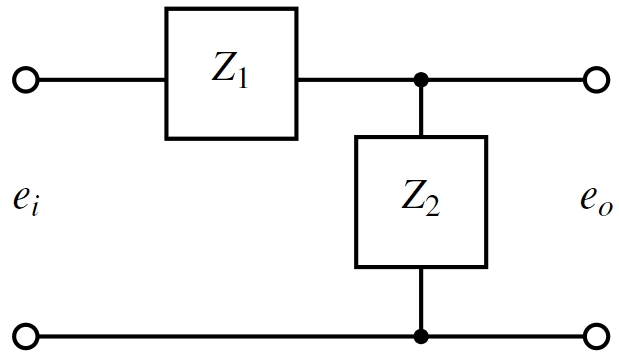
\includegraphics[width=.3\textwidth]{Chapter3/ComplexImpedencecircuit.png} %1.png是图片文件的相对路径
    \caption{Circuit consists of Complex Impedance} %caption是图片的标题
    \label{ComplexImpedancecircuit} %此处的label相当于一个图片的专属标志,目的是方便上下文的引用
\end{figure}

图\ref{ComplexImpedancecircuit}所示的是由复阻抗值分别为Z1和Z2的元件所组成的复阻抗电路,对于这个电路,其传输函数为:
\begin{equation}
    \frac{E_o(s)}{E_i(s)}=\frac{Z_2(s)}{Z_1(s)+Z_2(s)}
\end{equation}

以图\ref{LRCcircuit}所示电路为例。根据图\ref{LRCcircuit}可知,此时$Z_1=Ls+R$,$\frac{1}{Cs}$,带入上式可得传输函数为:
\begin{equation}
    \frac{E_o(s)}{E_i(s)}=\frac{\frac{1}{Cs}}{Ls+R+\frac{1}{Cs}}=\frac{1}{LCs^2+RCs+1}
\end{equation}

\begin{figure}
    \centering
    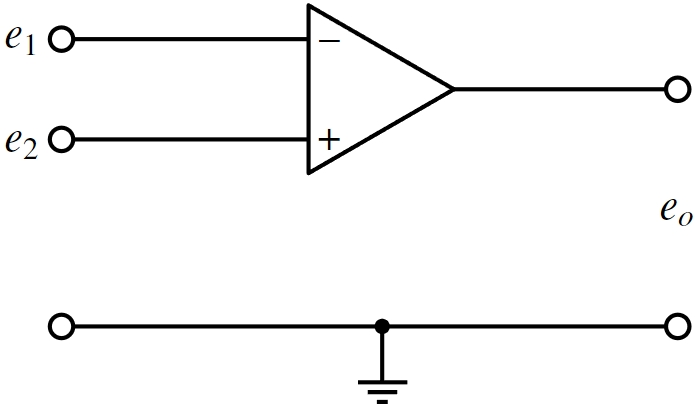
\includegraphics[width=.4\textwidth]{Chapter3/Opa.png} %1.png是图片文件的相对路径
    \caption{Operational amplifier} %caption是图片的标题
    \label{Operational amplifier} %此处的label相当于一个图片的专属标志,目的是方便上下文的引用
\end{figure}

图\ref{Operational amplifier}所示的是一个典型的运算放大器的电路图,其输入输出关系为:
\begin{equation}
    e_o(t)=K(e_2(t)-e_1(t))=-K(e_1(t)-e_2(t))
\end{equation}
对于一个运算放大器而言,其理想情况下的输入阻抗应为无穷大,输出阻抗应为0(向前一级拿的多,自己消耗的少),然而实际情况中输入和输出阻抗做不到上述要求,因此会存在非常小的输入电流,并且后级会对输出产生略微的影响,即会存在对前一级的负载效应,同时后一级对运算放大器也会产生负载效应,但所产生的影响非常小基本可以被忽略,因此近似为无负载效应进行分析。

\begin{formal}
    反相放大器
\end{formal}

\begin{figure}
    \centering
    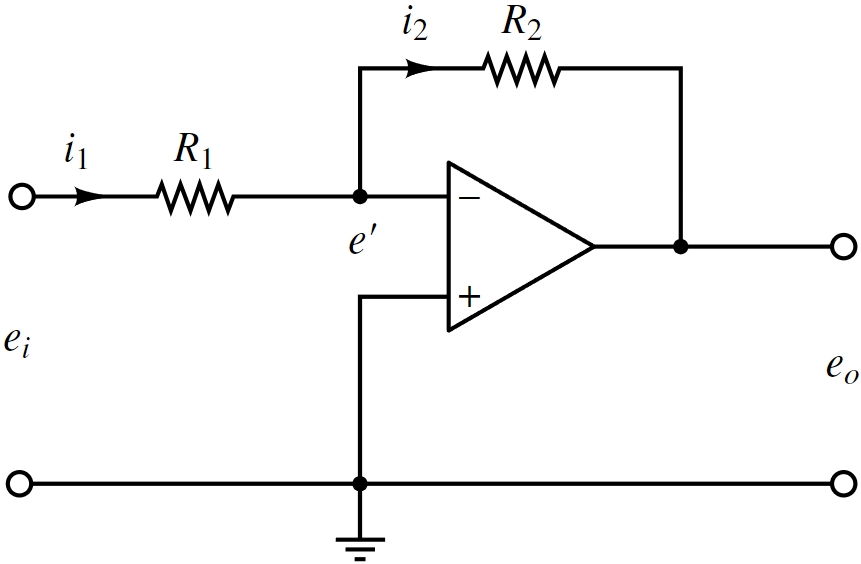
\includegraphics[width=.4\textwidth]{Chapter3/InverterAmplifier.png} %1.png是图片文件的相对路径
    \caption{Inverting amplifier} %caption是图片的标题
    \label{Inverting amplifier} %此处的label相当于一个图片的专属标志,目的是方便上下文的引用
\end{figure}

图\ref{Inverting amplifier}所示的是反相放大电路,根据图\ref{Inverting amplifier}可知,该电路为负反馈电路,当运算放大器增益为无穷大时,电路处于深度负反馈,则该电路满足“虚短”、“虚断”,即有e`=0;又因为运算放大器输入电流基本为0,因此可得:
\begin{equation}
    e_o=-\frac{R2}{R1}e_i
\end{equation}

当R1=R2时,$e_o=-e_i$,即此时该电路仅作符号反相功能。

\begin{formal}
    同相放大器
\end{formal}

\begin{figure}
    \centering
    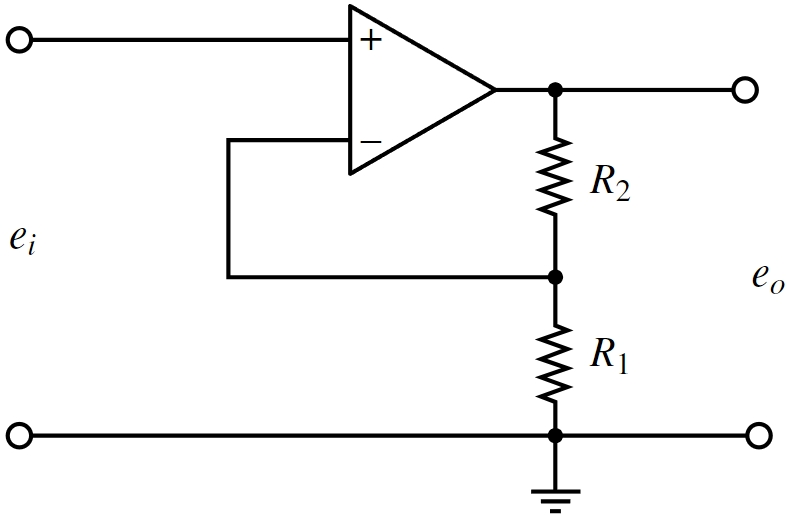
\includegraphics[width=.4\textwidth]{Chapter3/NoninvertingAmplifier.png} %1.png是图片文件的相对路径
    \caption{Noninverting amplifier} %caption是图片的标题
    \label{Noninverting amplifier} %此处的label相当于一个图片的专属标志,目的是方便上下文的引用
\end{figure}

图\ref{Noninverting amplifier}所示的是同相放大电路,根据图\ref{Noninverting amplifier}可知,该电路为负反馈电路,当运算放大器增益为无穷大时,电路处于深度负反馈,则该电路满足“虚短”、“虚断”,又因为运算放大器输入电流基本为0,因此可得:
\begin{equation}
    e_o=(1+\frac{R_2}{R_1})e_i
\end{equation}

\begin{figure}
    \centering
    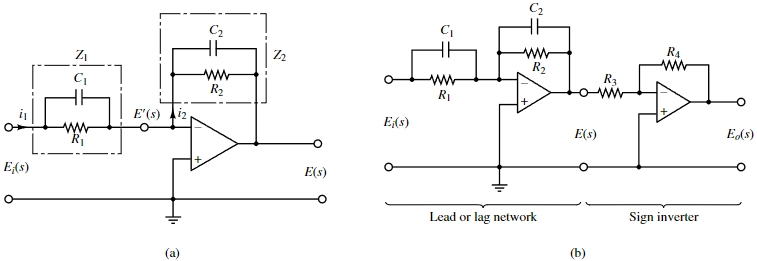
\includegraphics[width=.9\textwidth]{Chapter3/LeadorLagnetwork.png} %1.png是图片文件的相对路径
    \caption{Lead or Lag networks using operational Amplifiers} %caption是图片的标题
    \label{LeadorLagnetwork} %此处的label相当于一个图片的专属标志,目的是方便上下文的引用
\end{figure}

图\ref{LeadorLagnetwork}所示的是使用运算放大器的超前/滞后电路。根据图\ref{LeadorLagnetwork}(a)所示电路,复阻抗Z1和Z2为:
\begin{equation}
    Z_1=\frac{R_1}{R_1C_1s+1}, \quad Z_2=\frac{R_2}{R_2C_2s+1}
\end{equation}

因此其传输函数为:
\begin{equation}
    \frac{E(s)}{E_i(s)}=-\frac{Z_2}{Z_1}=-\frac{C_1}{C_2}\frac{s+\frac{1}{R_1C_1}}{s+\frac{1}{R_2C_2}}
\end{equation}

由于其传输函数中存在负号,因此这个电路会导致符号反相(?)。如果所需要的是同相信号,只要通过在其输入或输入端施加一级反相电路就可以解决负号问题,即如图\ref{LeadorLagnetwork}(b)所示。图\ref{LeadorLagnetwork}(b)所示电路的传输函数为:
\begin{equation}
        \frac{E_o(s)}{E_i(s)}=K_c\alpha \frac{Ts+1}{\alpha Ts+1}=K_c\frac{s+\frac{1}{T}}{s+\frac{1}{\alpha T}}\label{leadorlag}
\end{equation}

其中,$T=R1C1$,\quad $\alpha T=R2C2$,\quad $K_c=\frac{R4C1}{R3C2}$。
即$K_c\alpha =\frac{R2R4}{R1R3}$,\quad $\alpha =\frac{R2C2}{R1C1}$

通过对该电路的传输函数进行逆变换可以发现,该系统的微分方程中,输出和输入的未求导项的比值为$K_c\alpha$,因此该电路的dc增益为$K_c\alpha$(?)

此外,根据该电路的传输函数Eq.\ref{leadorlag}可知,当$R1C1>R2C2$时,相角大于0,此时电路表现出超前特性;当$R1C1<R2C2$时,相角小于0,此时电路表现出滞后特性。

\begin{formal}
    使用运算放大器的比例-积分-微分(PID)控制器
\end{formal}

\begin{figure}
    \centering
    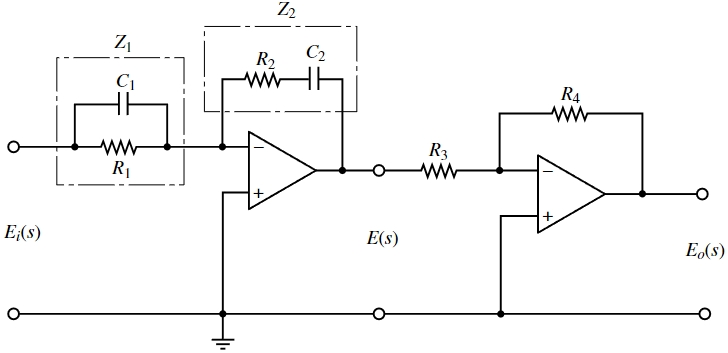
\includegraphics[width=.7\textwidth]{Chapter3/PIDController.png} %1.png是图片文件的相对路径
    \caption{PID Controller} %caption是图片的标题
    \label{PID Controller} %此处的label相当于一个图片的专属标志,目的是方便上下文的引用
\end{figure}

图\ref{PID Controller}所示的是比例-积分-微分(PID)控制器电路,通过分析其传输函数为:
\begin{equation}
    \begin{split}
        \frac{E_o(s)}{E_i(s)}&=\frac{R4(R1C1+R2C2)}{R3R1C2}[1+\frac{1}{(R1C1+R2C2)s}+\frac{R1C1R2C2}{R1C1+R2C2}s]\\
        &=K_p(1+\frac{T_i}{s}+T_ds)\\
        &=K_p+\frac{K_i}{s}+K_ds
    \end{split}
\end{equation}
其中$K_p$为proportional gain,$T_i$为integral time,$T_d$为derivative time,$K_i$为integral gain,$K_d$为derivative gain。

其他类型的运算放大器电路及其传输函数如图\ref{circuittable3-1}所示:
\begin{figure}
    \centering
    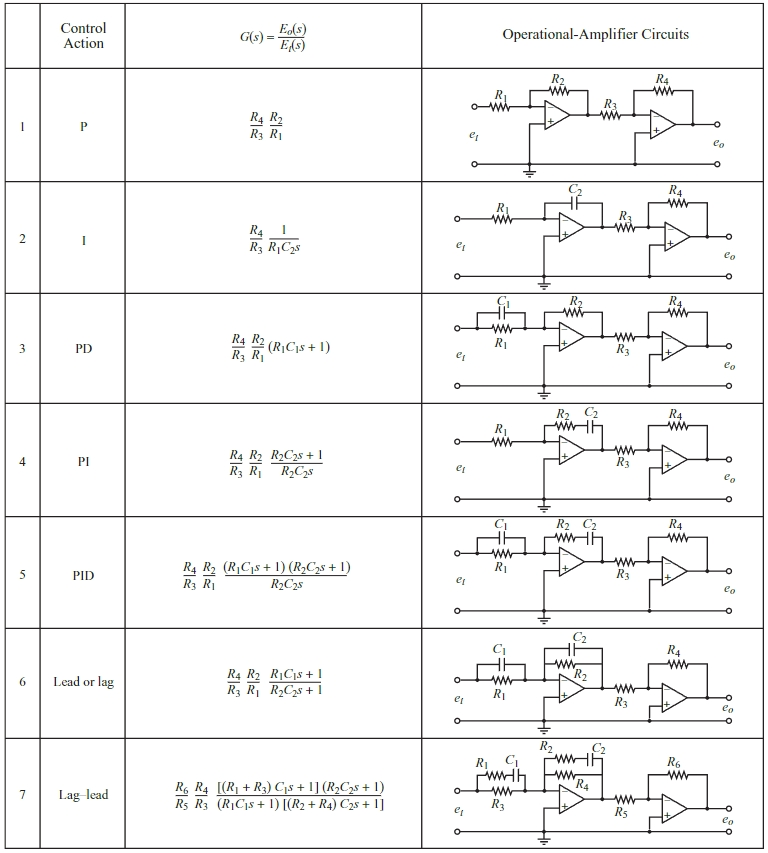
\includegraphics[width=1\textwidth]{Chapter3/table.png} %1.png是图片文件的相对路径
    \caption{不同类型的运算放大器电路及其传输函数} %caption是图片的标题
    \label{circuittable3-1} %此处的label相当于一个图片的专属标志,目的是方便上下文的引用
\end{figure}

\newpage

\section{流体系统和热系统的数学模型}

\newpage

\section{瞬态及稳态响应分析}
\subsection{引言}

对于一个系统而言,它实际上只具备一个功能,就是将输入信号进行处理转化为输出信号,因此系统的性能,实际就是对于信号的处理能力,而这一处理能力的直接体现就是输出信号自身的动态特性(例如输出信号的上升时间、峰值时间、建立时间...)及输出信号与输入信号之间的关系(例如输出与输入信号间的传输延迟、输出与输入信号间的增益...)。因此通过输出信号自身的动态特性及输出信号与输入信号之间的关系,我们就可以明确这个系统的处理能力。如果系统的处理能力好,则称这个系统具有高性能,如果系统的处理能力不好,则称这个系统具有低性能。

由于一个系统的动态特性可以通过相应的数学模型的进行描述,因此通过求解系统的数学模型,我们就可以得到系统的输出信号自身的动态特性及输出信号与输入信号之间的关系,从而对系统的性能进行分析。

如果一个系统对于任意类型的输入信号都能很好的进行处理,即总是具有高性能,那当然是最好的,但是这是非常难以实现的。

因此,我们选择抓住主要矛盾,即针对这个系统在正常工作情况下最频繁遇到的类型的信号的处理能力进行分析,只要求在其正常工作时能够对最频繁遇到的类型的输入信号进行很好的处理、具有高性能就足够了。

因此在设计系统时,我们会选择使用系统在正常工作情况下最频繁遇到的信号类型中的具有代表性且便于分析的信号作为测试信号。通过测试信号作用下输出信号自身的动态特性及输出信号与输入信号之间的关系,我们可以设计出这类输入信号作用时具有高性能的系统。例如:如果系统实际工作时的输入是一个随时间变化的信号,我们会选择使用ramp function作为输入信号对系统性能进行测试;如果系统实际工作时的输入是一个瞬时扰动,则会选择使用step function作为输入信号对系统性能进行测试;如果系统实际工作时的输入是一个具有瞬时高能量的信号,则会选择使用impulse function作为输入信号对系统性能进行测试。

当基于上述方法设计出具有某一性能的系统之后,需要与其他系统之间进行性能比较时,我们需要设定一个比较的基准。一般而言,这个基准会被设置为相同的测试输入信号,通过判断相同的测试输入信号作用下的系统的输出信号自身的动态特性及输出信号与输入信号之间的关系,从而对各个系统之间的性能进行比较。

其中,输出信号自身的动态特性及输出信号与输入信号之间的关系均可以通过输出信号的响应表达式得到。因此我们只要求解出输出信号的响应表达式,就可以获得输出信号自身的动态特性及输出信号与输入信号之间的关系,并最终实现上述的单个系统的性能判断和多个系统的性能比较。

\begin{formal}
    瞬态响应(Transient Response)和稳态响应(Steady-State Response):
    \begin{itemize}
        \item 瞬态响应:从始态持续到终态的响应(By transient response, we mean that which goes from the initial state to the final state)。对应的是响应的函数中会随着时间增大衰减为0的项。
        \item 稳态响应:时间趋于无穷大时系统表现出的响应(By steady-state response, we mean the manner in which the system output behaves as
        t approaches infinity)。对应的是响应的函数中不会随着时间增大衰减为0的项。
    \end{itemize}

    根据上述定义可知,任意一个响应$c(t)$都可以写为:
    \begin{equation}
        c(t)=c_{ss}(t)+c_{tr}(t)
    \end{equation}

    其中$c_{ss}(t)$为稳态响应,$c_{tr}(t)$为瞬态响应。
\end{formal}

在后文中,将会对一阶、二阶、高阶系统针对不同输入信号的输出响应进行推导,需要注意的是,后文的推导都是基于初始条件为0得到的,因此得到的输出响应表达式只适用于初始条件为0的情况,其余初始条件下的输出响应表达式与后文推导得来的并不相同。

由于初始条件为0,因此系统的传输函数满足$G(s)=Y(s)/U(s)=Y(s)/X(s)$,$U(s)=X(s)$,其中$X(s)$为所施加输入信号在零状态时的拉普拉斯变换。

\begin{figure}
    \centering
    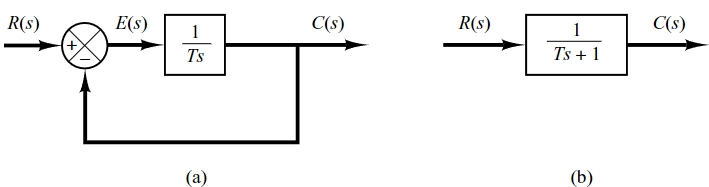
\includegraphics[width=.9\textwidth]{Chapter5/1ordersystem.png} %1.png是图片文件的相对路径
    \caption{一阶系统框图} %caption是图片的标题
    \label{1ordersystem} %此处的label相当于一个图片的专属标志,目的是方便上下文的引用
\end{figure}

\subsection{一阶系统}
以图\ref{1ordersystem}所示一阶系统为例,其传输函数为(该一阶系统传输函数具有普遍适用性,任意一阶传输函数都可写成“系数*下式中的传输函数$G(s)$”):
\begin{equation}
    \frac{C(s)}{R(s)}=G(s)=\frac{1}{Ts+1}
\end{equation}

\begin{formal}
    一阶系统单位阶跃输入时的输出响应
\end{formal}
    当初始条件为0时,单位阶跃函数的拉普拉斯变换为:$1/s$,因此输出响应的拉普拉斯表达式为:
    \begin{equation}
        C(s)=\frac{1}{Ts+1}\frac{1}{s}=\frac{1}{s}=\frac{1}{s+(1/T)}
    \end{equation}

    在初始条件为0的情况下对上述输出函数进行拉普拉斯逆变换可得输出函数的时域表达式为:
    \begin{equation}
        c(t)=1-e^{-t/T} \quad for \quad t ≥ 0
    \end{equation}

    \begin{figure}
        \centering
        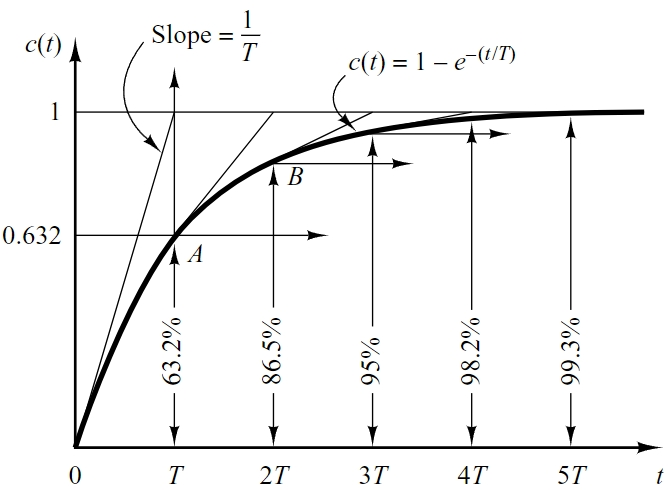
\includegraphics[width=.5\textwidth]{Chapter5/1orderunitstepresponse.png} %1.png是图片文件的相对路径
        \caption{一阶系统单位阶跃输入时的输出响应} %caption是图片的标题
        \label{1orderunitstepresponse} %此处的label相当于一个图片的专属标志,目的是方便上下文的引用
    \end{figure}
    
    从上述c(t)的表达式可以看出,该系统在输入为单位阶跃函数时输出响应是从0逐渐变化到1的,并在t=T时刻达到上升至最终值的63.2\% ,在t=3T时达到最终值的95\%,在t=4T时达到最终值的98.2\%。

    因此时间常数T越小,一阶系统单位阶跃输入所对应的输出响应变化越快。同时如图\ref{1orderunitstepresponse}所示,在t=0时刻,输出响应的曲线斜率为$1/T$。

    此外,从图\ref{1orderunitstepresponse}可以看出,输出随着时间的增大不断接近于最终值,但是完全到达最终值需要无穷长的时间,因此如果到达最终值的时间去代表系统到达稳态的响应时间是不合理的,一般采用的方法为当输出响应的值达到[(1-2\%)最终值,(1+2\%)最终值]这个范围所需的时间,从图\ref{1orderunitstepresponse}可以看出,这个时间近似对应于4T.

    对于其他的一阶系统而言,其输出响应与该系统的输出响应的区别仅在于对上述求出的c(t)表达式乘以对应的系数,这个系数就是其他一阶系统传输函数转化为上述系统传输函数的形式的过程中多出来的系数(因为系数在拉普拉斯正逆变换过程中不会改变).

    也因此不同一阶系统的输出响应其实只是在该系统的输出响应前乘以一项常系数,其余所有性质均是相同的.这一点对于任何输入信号都是适用的.

\begin{formal}
    一阶系统单位斜坡输入时的输出响应
\end{formal}
当初始条件为0时,单位斜坡函数的拉普拉斯变换为:$1/s^2$,因此输出响应的拉普拉斯表达式为:
\begin{equation}
    C(s)=\frac{1}{Ts+1}\frac{1}{s^2}=\frac{1}{s^2}-\frac{T}{s}+\frac{T^2}{Ts+1}
\end{equation}

在初始条件为0的情况下对上述输出函数进行拉普拉斯逆变换可得输出函数的时域表达式为:
\begin{equation}
    c(t)=t-T+Te^{-t/T} \quad for \quad t ≥ 0
\end{equation}

所以图\ref{1ordersystem}中的误差信号$E(s)$的时域表达式为:
\begin{equation}
    \begin{split}
        e(t)&=\mathscr{L}^{-1}[E(s)]\\
        &=\mathscr{L}^{-1}[R(s)-C(s)]\\
        &=\mathscr{L}^{-1}[R(s)]-\mathscr{L}^{-1}[C(s)]\\
        &=r(t)-c(t)\\
        &=T(1-e^{-t/T})
    \end{split}
\end{equation}

根据$e(t)$的表达式可知,当时间趋于无穷大时,$e(∞)=T$,T越小,稳态误差$e(t)$越小.图\ref{1orderunitrampresponse}所示的是该系统在单位斜坡函数输入下,输入与输出信号的函数曲线.
\begin{figure}
    \centering
    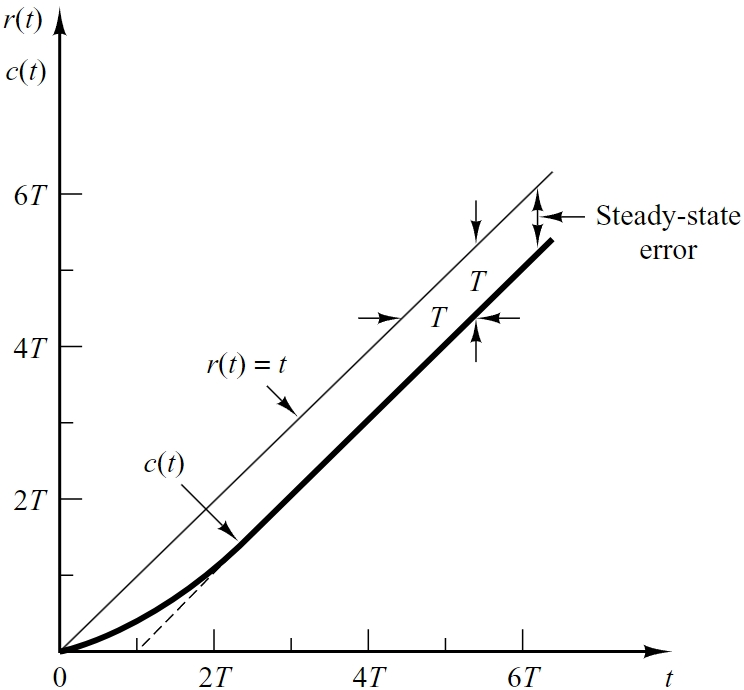
\includegraphics[width=.5\textwidth]{Chapter5/1orderunitrampresponse.png} %1.png是图片文件的相对路径
    \caption{一阶系统单位斜坡输入时的输出响应} %caption是图片的标题
    \label{1orderunitrampresponse} %此处的label相当于一个图片的专属标志,目的是方便上下文的引用
\end{figure}

\begin{formal}
    一阶系统单位冲激输入时的输出响应
\end{formal}
当初始条件为0时,单位冲激函数的拉普拉斯变换为:$1$,因此输出响应的拉普拉斯表达式为:
\begin{equation}
    C(s)=\frac{1}{Ts+1}
\end{equation}

在初始条件为0的情况下对上述输出函数进行拉普拉斯逆变换可得输出函数的时域表达式为:
\begin{equation}
    c(t)=\frac{1}{T}e^{-t/T}    \quad for \quad t ≥ 0
\end{equation}

图\ref{1orderunitimpulseresponse}所示的是该系统在单位冲激函数输入下,输入与输出信号的函数曲线.
\begin{figure}
    \centering
    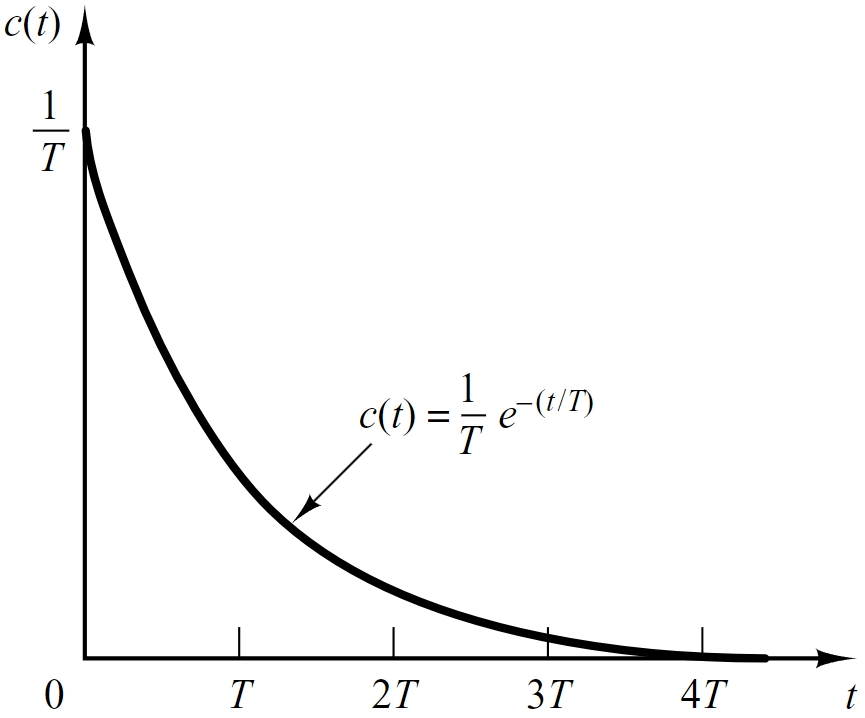
\includegraphics[width=.5\textwidth]{Chapter5/1orderunitumpulseresponse.png} %1.png是图片文件的相对路径
    \caption{一阶系统单位冲激输入时的输出响应} %caption是图片的标题
    \label{1orderunitimpulseresponse} %此处的label相当于一个图片的专属标志,目的是方便上下文的引用
\end{figure}

从上述三种输入信号所对应的输出响应的表达式可以发现,如果输入信号之间是导数关系,那么它们所产生的输出响应之间也将是导数关系,如果输入信号之间是积分关系,那么它们所产生的输出响应之间也将是积分关系.这一方法是通过拉普拉斯的微分性质推导得来的,它仅适用于初始条件为0的LTI系统,其他情况下这一方法并不适用.


\subsection{二阶系统}
\begin{figure}
    \centering
    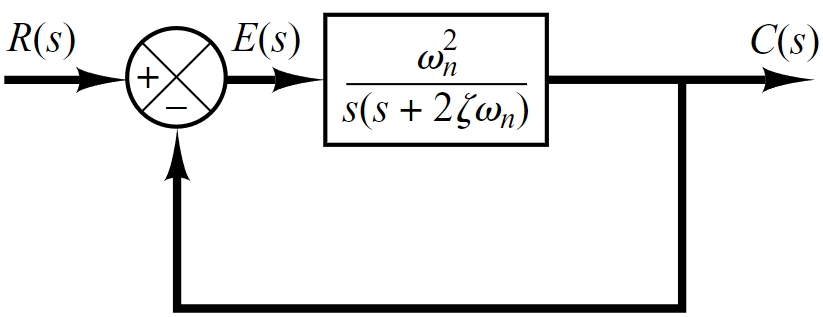
\includegraphics[width=.5\textwidth]{Chapter5/2ordersystem.png} %1.png是图片文件的相对路径
    \caption{二阶系统框图} %caption是图片的标题
    \label{2ordersystem} %此处的label相当于一个图片的专属标志,目的是方便上下文的引用
\end{figure}

以图\ref{2ordersystem}所示二阶系统为例,其传输函数为(这个系统的传输函数具备普遍适用性):
\begin{equation}
    \frac{C(s)}{R(s)}=G(s)=\frac{\omega _n^2}{s^2+2\zeta \omega _n s+\omega _n^2}
\end{equation}

这种形式的二阶传输函数称为二阶系统的标准传输函数,其中$\zeta$称为系统的阻尼比(damping ratio of the system),$\omega _n$称为无阻尼自然频率(undamped natural frequency).

当$\zeta = 0$时 该传输函数的极点位于s平面的$j\omega$轴上,系统的瞬态响应会保持等幅振荡,瞬态响应总是存在.

当$0<\zeta < 1$时 该传输函数的极点位于s平面的左半平面,系统的瞬态响应会进行减幅振荡,此时系统处于欠阻尼(underdamped)状态.

当$\zeta = 1$时 系统处于临界阻尼(critically damped)状态.

当$\zeta > 1$时 系统处于过阻尼(overdamped)状态.

(为什么不考虑负阻尼比的情况?)

\begin{formal}
    二阶系统单位阶跃输入时的输出响应
\end{formal}
(1) Underdamped case(0<$\zeta$<1)

当0<$\zeta$<1时,方程$s^2+2\zeta \omega _ns+\omega _n^2$的根是一对复共轭根,因此传输函数可以写为:
\begin{equation}
    \frac{C(s)}{R(s)}=\frac{\omega _n^2}{(s+\zeta \omega _n+j\omega _d)(s+\zeta \omega _n-j\omega _d)}
\end{equation}

其中$\omega_d=\omega_n \sqrt{1-\zeta ^2}$,$\omega_d$称为阻尼自然频率(damped natural frequency),当初始状态为0时,单位阶跃信号的传输函数为$1/s$,因此输出响应的拉普拉斯表达式为:
\begin{equation}
    \begin{split}
        C(s)&=\frac{\omega_n^2}{(s^2+2\zeta\omega_ns+\omega_n^2)s}\\
        &=\frac{1}{s}-\frac{s+\zeta\omega_n}{(s+\zeta\omega_n)^2+\omega_d^2}-\frac{\zeta\omega_n}{(s+\zeta\omega_n)^2+\omega_d^2}\\
        &=\frac{1}{s}-\frac{s+\zeta\omega_n}{(s+\zeta\omega_n)^2+\omega_d^2}-\frac{\zeta}{\sqrt{1-\zeta^2}}\frac{\omega_d}{(s+\zeta\omega_n)^2+\omega_d^2}
    \end{split}
\end{equation}

根据拉普拉斯的复频移性质,并对上述拉普拉斯表达式进行逆变换可以得到输出函数的时域表达式为:
\begin{equation}
    \begin{split}
        c(t)=\mathscr{L}[C(s)]&=1-e^{-\zeta\omega_nt}[cos(\omega_dt)+\frac{\zeta}{\sqrt{1-\zeta^2}}sin(\omega_dt)]\\
        &=1-\frac{e^{-\zeta\omega_nt}}{\sqrt{1-\zeta^2}}sin(\omega_dt+tan^{-1}(\frac{\sqrt{1-\zeta^2}}{\zeta})) \quad for \quad t≥0\label{underdampedoutputfunction}
    \end{split}
\end{equation}

从上式中可以发现,振荡项的振动频率是$\omega_d$,并且$\omega_d$是随着阻尼比$\zeta$变化而变化的;此外在欠阻尼状态下,由于$\zeta \omega_n$总是大于0,因此振荡项是减幅振荡的并最终减幅为0.

图\ref{2ordersystem}系统中的误差信号e(t)为:
\begin{equation}
    \begin{split}
        e(t)&=\mathscr{L}^{-1}[E(s)]\\
        &=\mathscr{L}^{-1}[R(s)]-\mathscr{L}^{-1}[C(s)]\\
        &=r(t)-c(t)\\
        &=e^{-\zeta\omega_nt}[cos(\omega_dt)+\frac{\zeta}{\sqrt{1-\zeta^2}}sin(\omega_dt)] \quad for \quad t≥0
    \end{split}
\end{equation}

从上式可以看出,误差信号$e(t)$同样展现出了阻尼振荡特性,其中的振荡项也在进行减幅振荡,当时间趋于无穷时,最终$e(t)=0$.

当 $\zeta=0$时,带入方程Eq.\ref{underdampedoutputfunction},可得(因为这种情况下方程$s^2+2\zeta \omega _ns+\omega _n^2$的根也是一对复共轭根,因此推导过程完全一致,所以可以直接带入):
\begin{equation}
    c(t)=1-cos(\omega_nt), \quad for \quad t≥0 \label{umdumpoutputfunction}
\end{equation}

通过Eq.\ref{umdumpoutputfunction}可以发现,当$\zeta=0$时,振荡项的频率为$\omega_n$,即无阻尼自然频率.换句话说,$\omega_n$的定义也就是$\zeta=0$即系统没有阻尼时的振荡频率.

通过方程Eq.\ref{underdampedoutputfunction}和Eq.\ref{umdumpoutputfunction}可知,如果一个系统存在阻尼量,则我们实验所能观测到的都是阻尼自然频率$\omega_d$,且$\omega_d=\omega_n*\sqrt{1-\zeta^2}$,这个频率总是低于无阻尼自然频率$\omega_n$,并会随着阻尼比$\zeta$的增大而减小,随着$\zeta$变得大于等于1,响应将不再振荡.

当$\zeta<0$时,$s^2+2\zeta \omega _ns+\omega _n^2$的根也是一对复共轭根,因此其分析过程和得到的结论与$0<\zeta<1$时的完全一致。

通过带入为负数的$\zeta$,我们发现输出响应中的指数项是随着时间增大而增大发散的,这样的响应是不可能趋于一个稳定状态的,且越来越大的响应很有可能会使整个系统崩溃,因此这样的系统是不稳定的。

(2)临界阻尼状态($\zeta=1$):如果传输函数的两个极点是相同的,则称系统处于临界阻尼状态.

在初始条件为0且输入信号为单位阶跃函数时,输出响应的拉普拉斯表达式为:
\begin{equation}
    C(s)=\frac{\omega_n^2}{(s+\omega_n)^2s}\label{criticaldumpoutputfunction}
\end{equation}

对上述拉普拉斯表达式进行逆变换可以得到输出函数的时域表达式为:
\begin{equation}
    c(t)=1-e^{-\omega_nt}(1+\omega_nt) \quad for \quad t≥0
\end{equation}

(3) 过阻尼状态($\zeta>1$):在这种情况下,传输函数的两个极点是负实数且不相等.当初始条件为0且输入信号为单位阶跃函数时:
\begin{equation}
    C(s)=\frac{\omega_n^2}{(s+\zeta\omega_n+\omega_n\sqrt{\zeta^2-1})(s+\zeta\omega_n-\omega_n\sqrt{\zeta^2-1})s}
\end{equation}

对上述拉普拉斯表达式进行逆变换可以得到输出函数的时域表达式为:
\begin{equation}
    c(t)=1+\frac{\omega_n}{2\sqrt{\zeta^2-1}}(\frac{e^{-s_1t}}{s_1}-\frac{e^{-s_2t}}{s_2})\label{overdampoutputfunction}
\end{equation}

其中$s_1=(\zeta + \sqrt{\zeta^2-1})\omega_n$,$s_2=(\zeta - \sqrt{\zeta^2-1})\omega_n$

对于上述时域表达式的形式可以从另外一个角度理解。由于在过阻尼状态($\zeta>1$)下,方程$s^2+2\zeta \omega _ns+\omega _n^2$具有两个实数根$p_1$和$p_2$,因此此时该系统的传输函数可以改写为:
\begin{equation}
    G(s)=\frac{C(s)}{R(s)}=\frac{a_1}{s+p_1}+\frac{a_2}{s+p_2}
\end{equation}

因此拉普拉斯形式下输出响应为:
\begin{equation}
    C(s)=\frac{a_1}{s+p_1}R(s)+\frac{a_2}{s+p_2}R(s)
\end{equation}

通过上式可以看出,在过阻尼状态($\zeta>1$)下,总的输出响应其实是输入通过两个不同的一阶系统产生的响应之和,通过一阶系统推导出的结果可知,输入通过一阶系统产生的响应是指数形式的,因此总的输出响应如Eq.\ref{overdampoutputfunction}所示为两个指数项之和。

输出函数Eq.\ref{overdampoutputfunction}中存在有两个指数衰减项,当$\zeta$远大于1时,有$s_1>>s_2$,此时$s_1$所对应的衰减项比$s_2$所对应的衰减项衰减的更快,即$e^{-s_1t}<<e^{-s_2t}$,因此可以忽略$s_1$所对应的指数相,即忽略$s_1$所对应的极点对系统产生的影响,从而将原本的二阶系统近似为一阶系统.

\begin{figure}
    \centering
    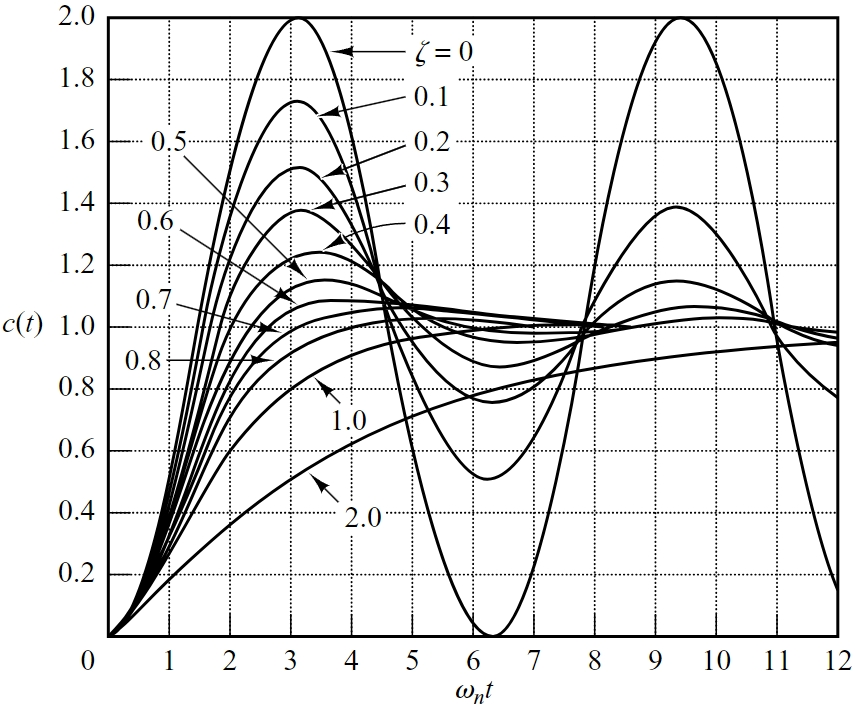
\includegraphics[width=.5\textwidth]{Chapter5/2orderunitstepresponse.png} %1.png是图片文件的相对路径
    \caption{二阶系统初始条件为0时单位阶跃输入的输出函数曲线} %caption是图片的标题
    \label{2orderunitstepresponse} %此处的label相当于一个图片的专属标志,目的是方便上下文的引用
\end{figure}

图\ref{2orderunitstepresponse}所示的是基于Eq.\ref{underdampedoutputfunction},Eq.\ref{criticaldumpoutputfunction}和Eq.\ref{overdampoutputfunction}得到的不同阻尼比条件下的输出函数曲线.从图\ref{2orderunitstepresponse}中可以看到,当$\zeta$处于0.5-0.8之间时输出函数相较于临界阻尼或过阻尼状态下的输出函数能够更快的接近终值;对于无振荡的输出函数而言,临界阻尼是最快能够接近终值的;过阻尼系统的输出无论对于任何输入总是反应最慢.

除此之外,从图\ref{2orderunitstepresponse}可以看出,随着$\zeta$越来越大,其输出函数的曲线接近一阶系统的输出函数曲线,也因此当$\zeta$无穷大时,我们可以用一阶系统近似分析该二阶系统.

通过Eq.\ref{underdampedoutputfunction}、Eq.\ref{criticaldumpoutputfunction}和Eq.\ref{overdampoutputfunction} 可以发现,在图\ref{2ordersystem}所示的标准二阶系统中,当初始条件为0且输入的信号为单位阶跃函数时,阻尼比$\zeta$的大小决定了输出响应的组成部分:当阻尼比处于[0,1)之间时,输出响应的组成部分里包含了“指数函数与三角函数相乘”项,当阻尼比处于[1,∞)之间时,输出响应的组成部分里包含了“指数函数”项(随着阻尼比越来越大,三角函数的振动频率越来越小,当阻尼比为1时,振动频率为0,因此会出现上述在阻尼比处于[1,∞)之间时输出响应的组成部分里只有“指数函数”项而不包括“指数函数与三角函数相乘”项的情况)。

但无论阻尼比是处于上述哪个范围,指数函数项的变量t(时间)前面的系数总是极点的实部,因此如果极点处于左半平面,则实部为负数,对应的项将不断衰减,如果极点处于右半平面,则实部为正数,对应的项将不断增大发散。

\begin{formal}
    瞬态响应指标定义
    \begin{itemize}
        \item Delay time($t_d$):响应首次达到半终值所需的时间.
        \item Rise time($t_r$):响应从某一个值上升到另一个值所需的时间.对于欠阻尼二阶系统,由于其振荡特性,该系统的上升时间通常被定义为首次从0\%终值上升至100\%终值所需的时间;对于过阻尼系统,该系统的上升时间通常被定义为首次从10\%终值上升至90\%终值所需的时间.
        \item Peak time($t_p$):响应首次过冲峰值所需要的时间.
        \item Maximum (percent) overshoot($M_p$):当稳态值为1时,Maximum overshoot指的是过冲的最大值与1之间的差值;当稳态值不为1时,通常选用Maximum percent overshoot去表示过冲的程度,其定义为:
        \begin{equation}
            Maximum\_percent\_overshoot=\frac{c(t_p)-c(∞)}{c(∞)}*100\%
        \end{equation}
        Maximum (percent) overshoot直接表明了系统的相对稳定性.
        \item Settling time($t_s$):响应到达并保持在终值附近某一范围内所需的时间,一般这一范围会用百分比得形式表示(usually 2\% or 5\%),settling time与控制系统中最大的时间常数相关.
    \end{itemize}
\end{formal}

\begin{figure}
    \centering
    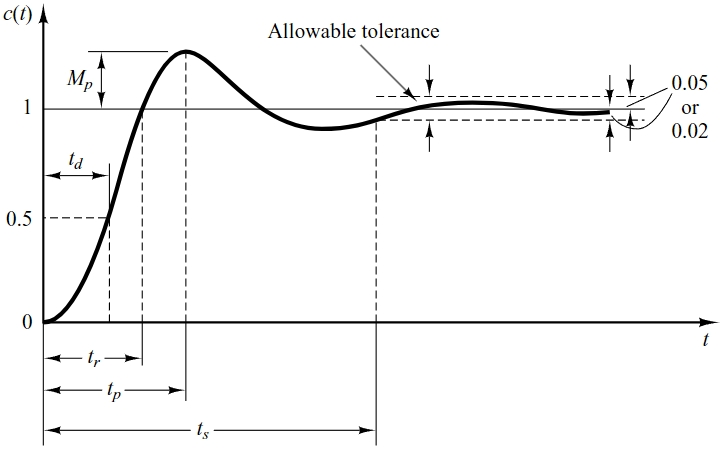
\includegraphics[width=.6\textwidth]{Chapter5/TransientResponseSpecification.png} %1.png是图片文件的相对路径
    \caption{单位阶跃输入时瞬态响应指标示意图} %caption是图片的标题
    \label{TransientResponseSpecification} %此处的label相当于一个图片的专属标志,目的是方便上下文的引用
\end{figure}

图\ref{TransientResponseSpecification}所示的是输入信号为阶跃函数时的瞬态响应指标示意图。(通常系统的性能指标会被设定为单位阶跃输入的瞬态响应)

上述所有指标并非都是必须的,需要根据实际的系统进行设定。例如对于过阻尼系统,它不会出现过冲振荡,因此不需要设置peak time和maximum overshoot的指标。

除了振荡器我们可以接受其响应是振荡的外,其余的系统我们更喜欢其响应变化是快且振荡小的(sufficiently damped),因此对于一个二阶系统而言,其阻尼比必须被设置在0.4-0.8之间。(阻尼比小响应快但过冲大,阻尼比大过冲小但响应慢,因此存在过冲幅度和响应速度之间的tradeoff)。

\begin{formal}
    二阶系统瞬态响应指标的求解方法
\end{formal}

以图\ref{2ordersystem}所示系统在:“1.underdamped($0<\zeta<1$),2.初始条件为0,3.输入信号为单位阶跃信号”这三个条件下系统的输出响应Eq.\ref{underdampedoutputfunction}为例.

(1)Rise time($t_r$):根据定义只要求下述方程并取最小的正解就可以求得rise time:
\begin{equation}
    c(t_r)=c(∞)
\end{equation}

在该例中为:$c(t_r)=1$

(2)Peak time($t_p$):根据定义只要求下述方程并取最小的正解就可以求得Peak time:
\begin{equation}
    \frac{dc}{dt}|_{t=t_p}=0
\end{equation}

在该例中为:$\frac{dc}{dt}|_{t=t_p}=0$,通过求解并取最小正解得到:$t_p=\frac{\pi}{\omega_d}$。此时我们发现,在该例中$t_p$等于以$\omega_d$为角频率的信号周期($T=\frac{2\pi}{\omega_d}$)的一半。

(3)maximum (percent) overshoot($M_p$):根据定义只要取$t=t_p$时刻的值并按照下述方程与终值比较就可以求得maximum (percent) overshoot:

当终值为1时:$M_p(maximum\_overshoot)=c(t_p)-1$

当终值不为1时:$M_p(maximum\_percent\_overshoot)=\frac{c(t_p)-c(∞)}{c(∞)}*100\%$

在该例中为:$M_p(maximum\_overshoot)=c(t_p)-1$

(4)Settling time($t_s$)

当响应的函数是随时间单调变化时,只需要通过下述方程就可求得settling time,其中a为相应的百分比要求:
\begin{equation}
    c(t_s)=(1-a\%)c(∞)
\end{equation}

当响应的函数是存在振荡时,可以用其满足的两条envelop function进行辅助求解。在该例中,根据Eq.\ref{underdampedoutputfunction}可得:
\begin{equation}
    1-\frac{e^{-\zeta \omega_nt}}{\sqrt{1-\zeta^2}}≤c(t)≤1+\frac{e^{-\zeta \omega_nt}}{\sqrt{1-\zeta^2}}
\end{equation}

因为c(t)总是在这两个函数所围的范围之间振荡,同时这两个函数又是单调函数,因此只要这两个函数到达了settling time所要求值的范围,那么c(t)一定到达了settling time所要求值的范围。

因此我们可以通过求两条envelop function到达settling time所需的时间近似求得c(t)到达settling time所需的时间。具体的如图\ref{settlingtime}所示

\begin{figure}
    \centering
    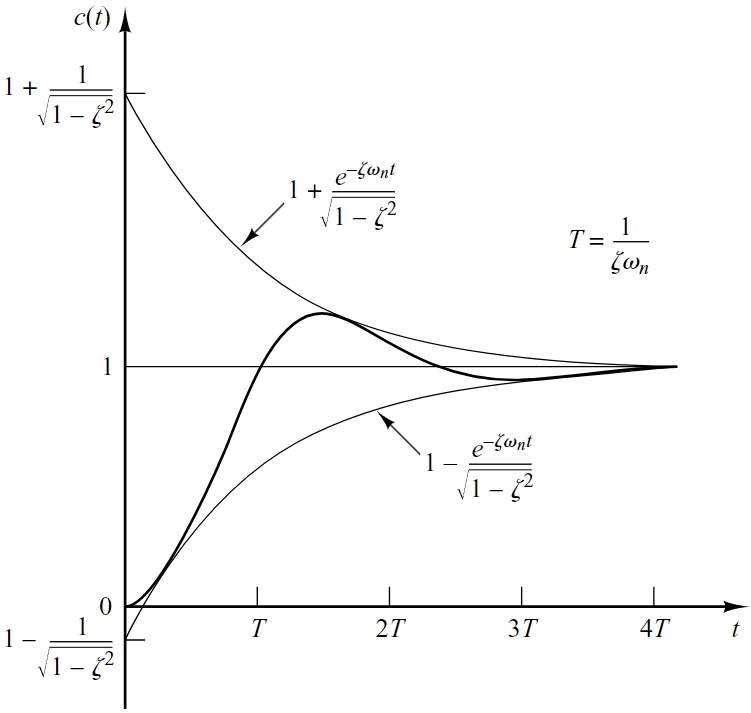
\includegraphics[width=.6\textwidth]{Chapter5/settlingtime.png} %1.png是图片文件的相对路径
    \caption{通过envelop function对具有振荡现象的响应进行settling time求解} %caption是图片的标题
    \label{settlingtime} %此处的label相当于一个图片的专属标志,目的是方便上下文的引用
\end{figure}

从图中我们可以看出,envelop function所对应的曲线与图\ref{1orderunitstepresponse}一阶系统的响应曲线十分相似,因此我们可以套用其结论:曲线在t=T时刻达到上升至最终值的63.2\% ,在t=3T时达到最终值的95\%,在t=4T时达到最终值的98.2\%,并利用这个结论得到近似的关于settling time的计算方法:

当要求是2\% criterion时:$t_s=4T$

当要求是5\% criterion时:$t_s=3T$

因为envelop的时间函数$T=\frac{1}{\zeta\omega_n}$,所以:当要求是2\% criterion时:$t_s=\frac{4}{\zeta\omega_n}$;当要求是5\% criterion时:$t_s=\frac{3}{\zeta\omega_n}$.

通过时间函数的表达式$T=\frac{1}{\zeta\omega_n}$可以发现settling time是由$\zeta$和$\omega_n$同时决定的,尽管$\zeta$已经受最大过冲指标所限制,我们仍可以通过调整$\omega_n$从而调整响应的settling time。

当然,通过将图\ref{settlingtime}和图\ref{1orderunitstepresponse}进行比较可以发现,两张图中的曲线并非完全相同,因此上述方法只能近似求得settling time,会存在误差。

\begin{formal}
    二阶系统单位冲激输入时的输出响应
\end{formal}
当初始条件为0时,单位冲激函数的拉普拉斯变化为$1$,因此拉普拉斯形式下的输出响应为:
\begin{equation}
    C(s)=\frac{\omega_n^2}{s^2+2\zeta\omega_ns+\omega_n^2}
\end{equation}

通过在不同$\zeta$范围内对上式进行拉普拉斯逆变换可得时域中的输出响应为:

For $0≤\zeta<1$
\begin{equation}
    c(t)=\frac{\omega_n}{\sqrt{1-\zeta^2}}e^{-\zeta\omega_nt}sin(\omega_n\sqrt{1-\zeta^2}t) \quad for \quad t≥0
\end{equation}

For$\zeta=1$
\begin{equation}
    c(t)=\omega_n^2te^{-\omega_nt} \quad for \quad t≥0
\end{equation}

For $\zeta>1$
\begin{equation}
    c(t)=\frac{\omega_n}{2\sqrt{\zeta^2-1}}e^{-(\zeta-\sqrt{\zeta^2-1})\omega_nt}-\frac{\omega_n}{2\sqrt{\zeta^2-1}}e^{-(\zeta+\sqrt{\zeta^2-1})\omega_nt}\quad for \quad t≥0
\end{equation}

当然除了上述计算方法外。由于单位冲激函数是单位阶跃函数的导数,因此在初始条件为0时,由单位冲激函数所产生的输出响应也可以通过对由单位阶跃函数所产生的输出响应求导得到。

\begin{figure}
    \centering
    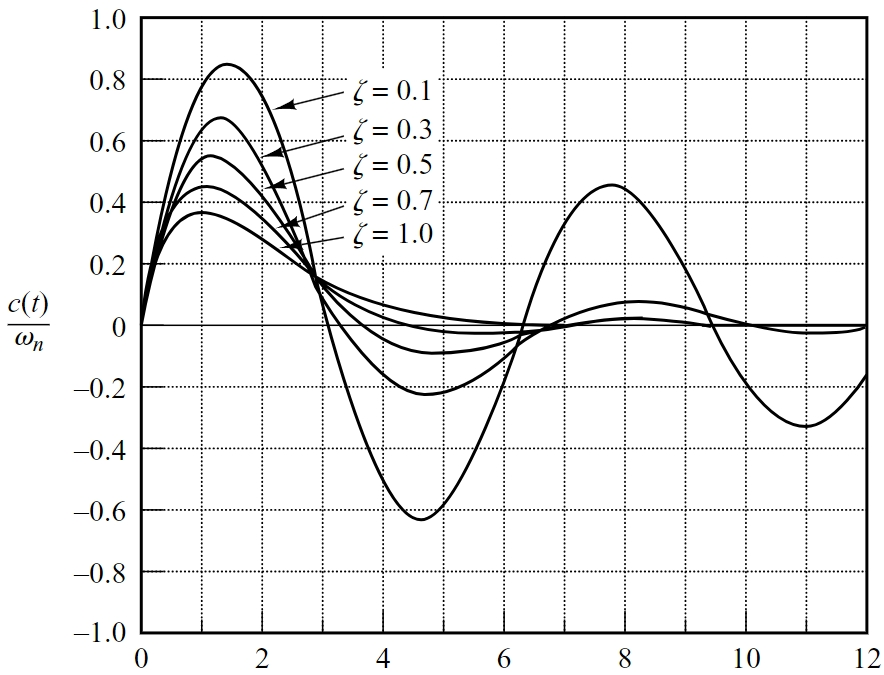
\includegraphics[width=.6\textwidth]{Chapter5/2orderunitimpulseresponse.png} %1.png是图片文件的相对路径
    \caption{初始条件为0情况下由单位脉冲函数引起的不同阻尼比的输出曲线} %caption是图片的标题
    \label{2orderunitimpulseresponse} %此处的label相当于一个图片的专属标志,目的是方便上下文的引用
\end{figure}

从图\ref{2orderunitimpulseresponse}可以看出,当$0≤\zeta<1$时,所产生的输出响应会围绕0上下振动,即c(t)既有正值又有负值;当$1≤\zeta$时,所产生的输出响应总是非负的,即$c(t)≥0$.


同时由于由单位冲激函数所产生的输出响应与通过对由单位阶跃函数所产生的输出响应之间的关系为导数关系。因此如果由单位冲激函数所产生的输出响应符号不发生改变,则由单位阶跃函数所产生的输出响应是单调变化的,说明这个系统处于临界阻尼或过阻尼状态。

如果由单位冲激函数所产生的输出响应符号发生改变,则该系统处于欠阻尼或零阻尼状态,其中由单位冲激函数所产生的输出响应的第一个正零点对应的就是由单位阶跃函数所产生的输出响应的peak time($t_p$),从0到由单位冲激函数所产生的输出响应的第一个正零点这一段范围内由单位冲激函数所产生的输出响应所围的面积就是由单位阶跃函数所产生的输出响应在t=$t_p$时刻的值$C_{unitstep}(t_p)$,假设由单位阶跃函数所产生的输出响应的稳态值为$C_{unitstep}(∞)$,则由单位阶跃函数所产生的输出响应的maximum percent overshoot=$\{[C_{unitstep}(t_p)-C_{unitstep}(∞)]/C_{unitstep}(∞)\}*100\%$,如果$C_{unitstep}(∞)=1$,则maximum overshoot=$C_{unitstep}(t_p)-1$。其具体如图\ref{2orderunitimpulseresponse2}所示。

\begin{figure}
    \centering
    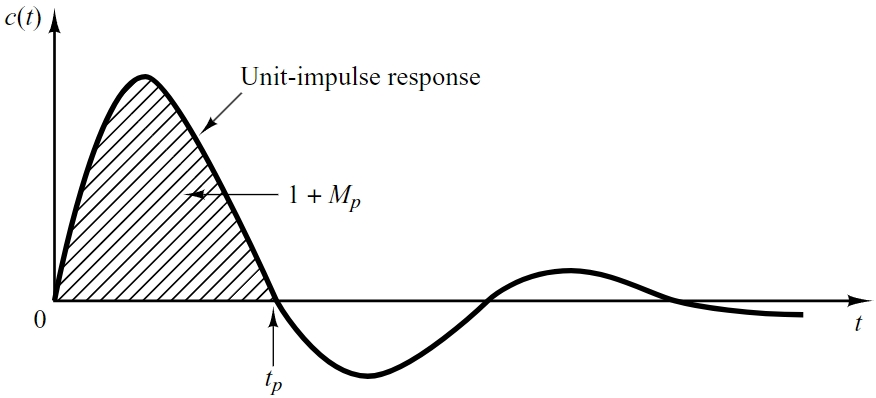
\includegraphics[width=.6\textwidth]{Chapter5/2orderunitimpulseresponse2.png} %1.png是图片文件的相对路径
    \caption{初始条件为0情况下由单位脉冲函数引起处于欠阻尼状态的输出曲线} %caption是图片的标题
    \label{2orderunitimpulseresponse2} %此处的label相当于一个图片的专属标志,目的是方便上下文的引用
\end{figure}

上述为由单位冲激函数所产生的输出响应与由单位阶跃函数所产生的输出响应的peak time和maximum (percent) overshoot之间的关系。对于由单位冲激函数所产生的输出响应自身的peak time为:
\begin{equation}
    t_p=\frac{tan^{-1}\frac{\sqrt{1-\zeta^2}}{\zeta}}{\omega_n\sqrt{1-\zeta^2}},\quad where\quad 0<\zeta<1
\end{equation}

\begin{equation}
    c(t)_{max}=\omega_nexp(-\frac{\zeta}{\sqrt{1-\zeta^2}}tan^{-1}\frac{\sqrt{1-\zeta^2}}{\zeta}),\quad where\quad 0<\zeta<1
\end{equation}

\subsection{高阶系统}

\begin{formal}
    高阶系统
\end{formal}

假设任意一个高阶系统的传输函数为:
\begin{equation}
    G(s)=\frac{C(s)}{R(s)}=\frac{b_0s^m+b_1s^{m-1}+...+b_{m-1}s+b_m}{a_0s^n+a_1s^{n-1}+...+a_{n-1}s+a_n}
\end{equation}

(1)当m小于n时(即传输函数为有理真分式)

通过部分分式展开法总是可以得到:
\begin{equation}
    G(s)=\frac{C(s)}{R(s)}=\sum_{x = 1}^{i}\frac{A_x}{s-p_x}+\sum_{y = 1}^{n-i}\frac{A_y}{s-s_y}
\end{equation}

其中$p_x$为实数,$s_y$为复数,$A_x$和$A_y$为对应项的系数。由于复数根具有共轭特性,因此(n-i)一定是偶数,且所有的复数一定可以两两匹配为复共轭根。假设$s_y=d_y+je_y$,因此:
\begin{equation}
    \sum_{y = 1}^{n-i}\frac{A_y}{s-s_y}=\sum_{y = 1}^{(n-i)/2}\frac{B_y}{s^2-2d_ys+(d_y^2+e_y^2)}
\end{equation}

其中$B_y$为共轭项的系数之积。例如:如果复数$s_y$与$s_k$互为复共轭根,则$B_y$=$A_y*A_k$。

则传输函数$G(s)$可以改写为:
\begin{equation}
    \begin{split}
        G(s)=\frac{C(s)}{R(s)}&=\sum_{x = 1}^{i}\frac{A_x}{s-p_x}+\sum_{y = 1}^{(n-i)/2}\frac{B_y}{s^2-2d_ys+(d_y^2+e_y^2)}\\
        &=\sum_{x = 1}^{i}\frac{-A_x}{p_x}\frac{1}{\frac{-1}{p_x}s+1}+\sum_{y = 1}^{(n-i)/2}\frac{B_y}{(d_y^2+e_y^2)}\frac{(d_y^2+e_y^2)}{s^2-2\frac{d_y}{\sqrt{d_y^2+e_y^2}}\sqrt{d_y^2+e_y^2}s+(d_y^2+e_y^2)}\\
        &=\sum_{x = 1}^{i}\frac{-A_x}{p_x}\frac{1}{Ts+1}+\sum_{y = 1}^{(n-i)/2}\frac{B_y}{(d_y^2+e_y^2)}\frac{\omega_n^2}{s^2-2\zeta\omega_ns+\omega_n^2}\label{highordertransferfunction}
    \end{split}
\end{equation}
其中$T=\frac{-1}{p_x}$,$\zeta=\frac{d_y}{\sqrt{d_y^2+e_y^2}}$,$\omega_n=\sqrt{d_y^2+e_y^2}$。

通过Eq.\ref{highordertransferfunction}可以看出任意高阶系统的传输函数都可以写为多个一阶系统和二阶系统传输函数的和。

因此当初始条件为0时,任意高阶系统在任意输入信号下的总时域响应就等于该输入信号分别通过多个一阶系统和二阶系统所产生的时域响应之和。

此外,根据前文中对传输函数为$\frac{1}{Ts+1}$的一阶系统和传输函数为$\frac{\omega_n^2}{s^2-2\zeta\omega_ns+\omega_n^2}$的二阶系统的分析结论和Eq.\ref{highordertransferfunction}中所示高阶传输函数的表达形式可知,系统的输出响应$c(t)$将总是由“常数项”、“指数函数项”、“指数函数与三角函数乘积项”以及“冲激函数的n阶导数项(其中$n≥0$)”组成,其中指数函数变量t(时间)前的系数为极点的“实部”。

证明:

(1)系统的输出响应$c(t)$将总是由“常数项”、“指数函数项”、“指数函数与三角函数乘积项”以及“冲激函数的n阶导数项(其中$n≥0$)”组成:

根据上述分析可知,任意高阶系统的传输函数都可以写为多个一阶系统和二阶系统传输函数的和,因此输入信号的拉普拉斯变换$R(s)$将与每个一阶系统和二阶系统的传输函数相乘,假设其中某一个乘积项为$K(s)$。

如果$K(s)$为有理真分式,则其一定可以像上述$G(s)$一样通过部分分式展开,根据拉普拉斯变换表对展开后的每一项的拉普拉斯逆变换一定是“常数项”、“指数函数项”、“指数函数与三角函数乘积项”其中一种,因此乘积项$K(s)$逆变换后的$k(t)$一定是“常数项”、“指数函数项”、“指数函数与三角函数乘积项”的组合。

如果$K(s)$为有理假分式,先通过多项式除法将其分为有理多项式和有理真分式,有理真分式部分根据上述分析可知其逆变换的结果是“常数项”、“指数函数项”、“指数函数与三角函数乘积项”的组合,有理多项式的逆变换的结果根据拉普拉斯变换表和拉普拉斯变换微积分性质可知一定是“冲激函数的n阶导数项(其中$n≥0$)”的组合。因此此时乘积项$K(s)$逆变换后的$k(t)$一定是“常数项”、“指数函数项”、“指数函数与三角函数乘积项”和“冲激函数的n阶导数项(其中$n≥0$)”的组合。

因此无论$K(s)$的形式如何,其拉普拉斯逆变换一定是“常数项”、“指数函数项”、“指数函数与三角函数乘积项”和“冲激函数的n阶导数项(其中$n≥0$)”的组合。

正如最初所述,高阶系统输出响应的拉普拉斯表达式是由多个不同的乘积项$K(s)$所组成,根据拉普拉斯变换的线性性质,高阶系统输出响应的拉普拉斯表达式逆变换后的时域表达式也一定是“常数项”、“指数函数项”、“指数函数与三角函数乘积项”和“冲激函数的n阶导数项(其中$n≥0$)”的组合。

(2)指数函数变量t(时间)前的系数为极点的“实部”

如果$K(s)$为有理真分式,则其一定可以像上述$G(s)$一样通过部分分式展开,即$K(s)=\sum_{x = 1}^{i}\frac{A_x}{s-p_x}+\sum_{y = 1}^{(n-i)/2}\frac{B_y}{s^2-2d_ys+(d_y^2+e_y^2)}=\sum_{x = 1}^{i}\frac{A_x}{s-p_x}+\sum_{y = 1}^{(n-i)/2}\frac{B_y}{(s-d_y)^2+e_y^2}$,根据拉普拉斯变换表及拉普拉斯变换的频移性质可知:系数$A_x$对应项的逆拉普拉斯变换形式为指数函数,其中指数项的系数是$p_x$,即极点的实部;系数$B_y$对应项的逆拉普拉斯变换形式为指数函数与三角函数乘积项,其中指数项的系数是$d_y$,即极点的实部。

如果$K(s)$为有理假分式,先通过多项式除法将其分为有理多项式和有理真分式,有理多项式的部分拉普拉斯变换后为“冲激函数的n阶导数项(其中$n≥0$)”,有理真分式部分的分析如上文所示。

因此无论$K(s)$的形式如何,其拉普拉斯逆变换中的“指数函数项”和“指数函数与三角函数乘积项”中的指数函数变量t(时间)前的系数总为极点的“实部”。

正如最初所述,高阶系统输出响应的拉普拉斯表达式是由多个不同的乘积项$K(s)$所组成,根据拉普拉斯变换的线性性质,高阶系统输出响应的拉普拉斯表达式逆变换后的时域表达式中“指数函数项”、“指数函数与三角函数乘积项”中的指数函数变量t(时间)前的系数一定为极点的“实部”。

因此当极点都处于左半平面时,指数函数变量t(时间)前的系数为负数,所有的“指数函数项”和“指数函数与三角函数乘积项”将不断衰减,当时间趋于无穷时,输出响应为所有的常数项之和。

而当存在有极点处于右半平面时,该极点对应的指数函数变量t(时间)前的系数为正数,这一项的值将会随着时间的增大而增大,进而导致输出响应不断增大,使得其无法趋于稳定状态;此外,越来越大的输出响应很有可能会使得整个系统崩溃。

因此对于一个系统而言,若要保证系统处于稳定状态,则其极点需要全部处于左半平面。一旦存在有极点处于右半平面,则该系统将不稳定。


(2)当m大于等于n时(即传输函数为有理假分式)
只需要通过多项式除法将传输函数分解为有理多项式$P(s)$和有理真分式$H(s)$,即$G(s)=P(s)+H(s)$,随后利用拉普拉斯变换的线性性质,分别求$P(s)$项和$H(s)$项进行分析计算就可以得到整体的输出响应。

其中$H(s)$的分析计算过程如第一种情况所述,即其所产生的输出响应项将包含“常数项”、“指数函数项”以及“指数函数与三角函数乘积项”。

对于$P(s)$而言,其包含的将是冲激函数的n阶导数项(其中$n≥0$)。

根据第一种情况中对输出响应的分析可知,这种情况下输出响应所包含的项也必然为“冲激函数的n阶导数项”、“常数项”、“指数函数项”以及“指数函数与三角函数乘积项”。

因此这种情况下系统稳定性的判断依据仍与上文所述一致:即只有当全部极点都处于左半平面时,系统才能保持稳定。

\subsection{Routh's Stability Criterion}
\begin{formal}
    Routh's Stability Criterion
\end{formal}

正如上文所述,系统的稳定性取决于极点是否全部都在左半平面,那么怎么判断系统的极点都在哪个位置呢?相较于对系统复杂的传输函数进行因式分解,劳斯稳定性判据可以直接通过特征方程的系数确认系统的根是否都在左半平面,即系统是否稳定。需要注意的是,劳斯稳定性判据只能适用于由“有限项”组成的多项式。

具体通过劳斯稳定性判据判断极点位置的流程如下:

1.写出拉普拉斯变换式的特征方程:

假设某一系统的拉普拉斯变换式$G(s)$为:$G(s)=\frac{C(s)}{R(s)}=\frac{b_0s^m+b_1s^{m-1}+...+b_{m-1}s+b_m}{a_0s^n+a_1s^{n-1}+...+a_{n-1}s+a_n}$,则其特征方程为:$a_0s^n+a_1s^{n-1}+...+a_{n-1}s+a_n=0$,其中$a_0,a_1,...,a_n$都为实数。

2.检查每一项前的系数:

由于特征方程总能写为有限个一次项$(s+a)$和二次项$(s^2+bs+c)$的乘积(可以证明其中$a,b,c$都是实数),所以只有当$a,b,c$都是正数时,所有的极点才会都在左半平面,因此特征方程的每一项前的系数都是相同符号是极点都在左半平面即系统稳定的必要非充分条件,因此如果存在有某一个特征方程中每一项前的系数的符号并不一致或存在某一个系数为0,那么这个特征方程的根一定存在有实部大于等于0的根,即该系统极点一定不全在左半平面,系统一定不稳定。

正如前文所说特征方程的每一项前的系数都是相同符号是极点都在左半平面即系统稳定的“必要非充分条件”,因此特征方程“每一项前的系数都是相同符号”并不能证明系统的极点都在左半平面即系统稳定,还需要进一步的进行判断。

3.对每一项前的系数进行排列

如果特征方程中每一项前的系数的符号都相同,如果所有的系数都是正数,则保持不变,如果所有的系数都是负数,则全部转化为正数。假设系数全部都转化为正数后的系统的特征方程为:$a_0s^n+a_1s^{n-1}+...+a_{n-1}s+a_n=0$,将其按照下述方式进行排列为矩阵,其中空着的项为0:
\begin{equation}
    \begin{matrix}
        s^n&a_0&a_2&a_4&a_6&...\\
        s^{n-1}&a_1&a_3&a_5&a_7&...\\
        s^{n-2}&b_1&b_2&b_3&b_4&...\\
        s^{n-3}&c_1&c_2&c_3&c_4&...\\
        s^{n-4}&d_1&d_2&d_3&d_4&...\\
        .&.&.\\
        .&.&.\\
        .&.&.\\
        s^{2}&e_1&e_2\\
        s^{1}&f_1\\
        s^{0}&g_1\\
    \end{matrix}\label{RouthStabilityMatrix}
\end{equation}

其中系数$b_1,b_2,b_3,...$,$c_1,c_2,b_3,...$,$d_1,d_2,d_3,...$...的定义为前其两行系数的交叉相乘,即:
\begin{equation}
    \begin{split}
        b_1&=\frac{a_1a_2-a_0a_3}{a_1}\\
        b_2&=\frac{a_1a_4-a_0a_5}{a_1}\\
        b_3&=\frac{a_1a_6-a_0a_7}{a_1}\\
        &.\\
        &.\\
        &.
    \end{split}
\end{equation}

\begin{equation}
    \begin{split}
        c_1&=\frac{b_1a_3-a_1b_2}{b_1}\\
        c_2&=\frac{b_1a_5-a_1b_3}{b_1}\\
        c_3&=\frac{b_1a_7-a_1b_4}{b_1}\\
        &.\\
        &.\\
        &.
    \end{split}
\end{equation}

\begin{equation}
    \begin{split}
        d_1&=\frac{c_1b_2-b_1c_2}{c_1}\\
        d_2&=\frac{c_1b_3-b_1c_3}{c_1}\\
        &.\\
        &.\\
        &.
    \end{split}
\end{equation}

劳斯稳定性判据表明,特征方程$a_0s^n+a_1s^{n-1}+...+a_{n-1}s+a_n=0$中具有正实部的根的数量等于矩阵\ref{RouthStabilityMatrix}中系数的第一列(即$a_1,b_1,...$所对应的一列)中符号变化的次数,例如如果所得到的矩阵只有三行,其中第一行为+,第二行为-,第三行为“+”,则符号变化了两次,即这个特征方程拥有两个具有正实部的根,因此判断是否有“实部为正的根”并不需要知道第一列中的具体数值,只需要知道它的符号就足够了,因此如果矩阵中某一行为了简化分析乘以或除以了一个正数,那么这一行为并不会对所得到的稳定性结论造成任何影响(从每一行系数的定义出发可以很容易得到证明)。

因此判断特征方程的根都在左半平面的充分必要条件为:特征方程所有的系数都是相同符号的且根据第三步所列出矩阵中系数的第一列的符号都是正号。

也因此如果特征方程中某一项前的系数与其他项不一样或为0,那么这个系统的极点一定不全在左半平面,那么这个系统一定不稳定。

特殊情况:

当第三步所求矩阵中系数的第一列中某一行的系数为0时,这个0项可以被一个非常小的正数$\epsilon$所取代以计算之后每行的数,例如如果某一系统的特征方程为:
\begin{equation}
    s^3+2s^2+s+2=0
\end{equation}

那么它在上述第三步中所得到的矩阵为:
\begin{equation}
    \begin{matrix}
        s^3&1&1\\
        s^2&2&2\\
        s^1&0≈\epsilon\\
        s^0&2
    \end{matrix}
\end{equation}

由于该特征方程的系数的符号完全相同且所得到的矩阵中符号改变的数量为0,所以该特征方程的根都在左半平面,即不存在实部为正的根,即系统稳定。

如果劳斯表中某一行全部为0,这就意味着该函数的特征方程在s平面中存在有径向对称幅值相同的根,即n对幅值相同符号相反的实根或n对共轭虚根。在这种情况下,如果要继续构建劳斯表,可以通过使用全0行上一行的系数组成辅助多项式,并对该辅助多项式求导,将求导得到的系数带入到全0行中,从而继续进行劳斯表的构建。

而前面所说的“n对幅值相同符号相反的实根或n对共轭虚根”,只要将辅助多项式转化为辅助方程,就可以通过求解该辅助方程得到。

因为根一定是偶数个,所以辅助方程一定是由$s^n$(n为偶数)所对应的行的系数构成的,所以全0行一定对应的是$s^n$(n为奇数)的行(这个总结对吗?)。

例如:如果一个系统的特征方程为:$s^5+2s^4+24s^3+48s^2-25s-50=0$。

直接写出的劳斯表为:
\begin{equation}
    \begin{matrix}
        s^5&1&24&-25\\
        s^4&2&48&-50\\
        s^3&0&0
    \end{matrix}
\end{equation}

可以看到$s^3$所对应的行全0,因此根据上文分析我们构建的辅助多项式为$P(s)=2s^4+48s^2-50$,所以$\frac{dP(s)}{ds}=8s^3+96s$,将求导得到的系数带入到$s^3$所对应的行中,并继续劳斯表的构建,最后可以得到该系统的劳斯表为:
\begin{equation}
    \begin{matrix}
        s^5&1&24&-25\\
        s^4&2&48&-50\\
        s^3&8&96\\
        s^2&24&-50\\
        s^1&112.7&0\\
        s^0&-50
    \end{matrix}
\end{equation}

通过对辅助方程$P(s)=2s^4+48s^2-50=0$进行求解,我们得到:$s=±1$ or $s=±j5$,经过检验我们发现,通过辅助方程求导的这四个根都属于特征方程的根,即都属于该系统的极点。

因此如果我们已知系统存在成对的共轭虚根或符号相反幅值相同的实根,我们可以通过构建劳斯表,并搭建辅助方程,进而快速求得这些根的值。这一点在第六章的根轨迹绘制中经常用到。

\begin{formal}
    相对稳定性分析
\end{formal}

上述内容介绍了通过劳斯稳定性判据对系统的绝对稳定性即极点是不是都处于左半平面进行判定。当系统稳定即所有极点都处于左半平面时,其相对稳定性也是我们需要考虑的。

假设$\hat{s}=s+\sigma $(其中$\sigma$为常数),将$\hat{s}$带入至原本的特征方程之中可以得到关于$\hat{s}$的多项式特征方程,对$\hat{s}$的多项式特征方程进行上述的劳斯稳定性判据可以确定原本的特征方程之中有多少个在$s=-\sigma$右侧的根,即系统有多少个在$s=-\sigma$右侧的极点。

\begin{formal}
    劳斯稳定性判据在控制系统分析中的应用
\end{formal}

如果某一个系统的传输函数中有一个参数是可变参数,那么我们可以通过劳斯稳定性判据确认使得系统稳定的可变参数的变化范围。

\begin{figure}
    \centering
    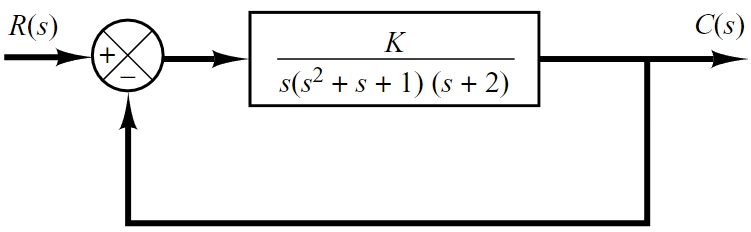
\includegraphics[width=.6\textwidth]{Chapter5/RouthApplication.png} %1.png是图片文件的相对路径
    \caption{具有可变参数的系统} %caption是图片的标题
    \label{RouthApplication} %此处的label相当于一个图片的专属标志,目的是方便上下文的引用
\end{figure}

以图\ref{RouthApplication}所示的系统为例,其传输函数为:
\begin{equation}
    \frac{C(s)}{R(s)}=\frac{K}{s(s^2+s+1)(s+2)+K}
\end{equation}

那么它的特征方程为:
\begin{equation}
    s^4+3s^3+3s^2+2s=K=0
\end{equation}

根据劳斯稳定性判据可知,特征方程如果要所有的根都在左半平面,则必须满足所有系数的符号相同,即$K>0$。

当$K>0$时,根据上文劳斯稳定性判据的判断过程,写出如下所示矩阵:
\begin{equation}
    \begin{matrix}
        s^4&1&3&K\\
        s^3&3&2&0\\
        s^2&\frac{7}{3}&K\\
        s^1&2-\frac{9}{7}K\\
        s^0&K
    \end{matrix}
\end{equation}

因为要所有的根都在左半平面,即实部为正数的根的数量为0,所以在系数的第一列中不能出现符号的改变,即$K>0$且$2-\frac{9}{7}K>0$,所以使得系统稳定的$K$的范围为$\frac{14}{9}>K>0$。

\subsection{积分和微分控制行为对系统性能的影响}
\begin{formal}
    积分控制行为对系统性能的影响:积分控制行为可以消除稳态误差$\lim_{t\rightarrow \infty}e(t)$,但会导致或衰减或发散的信号振荡现象。
\end{formal}

\begin{figure}
    \centering
    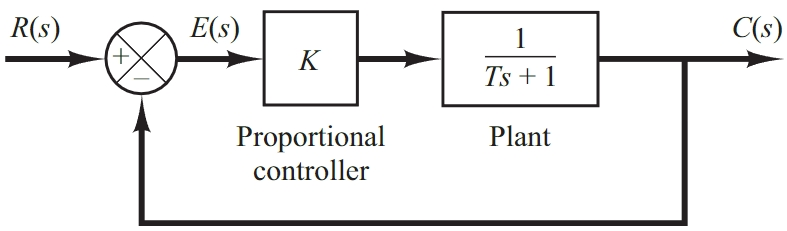
\includegraphics[width=.6\textwidth]{Chapter5/ProportionalControlSystem.png} %1.png是图片文件的相对路径
    \caption{比例控制系统} %caption是图片的标题
    \label{ProportionalControlSystem} %此处的label相当于一个图片的专属标志,目的是方便上下文的引用
\end{figure}

本节中的分析结论都是基于系统为稳定系统得到的。

以图\ref{ProportionalControlSystem}所示系统为例,假设初始条件为0,输入信号为单位阶跃信号,当系统中只具有比例控制功能而不具备积分控制功能时,该系统的传输函数为:
\begin{equation}
    G(s)=\frac{K}{Ts+1}
\end{equation}

因为:
\begin{equation}
    \frac{E(s)}{R(s)}=\frac{R(s)-C(s)}{R(s)}=1-\frac{C(s)}{R(s)}=\frac{1}{1+G(s)}
\end{equation}

所以:
\begin{equation}
    E(s)=\frac{Ts+1}{Ts+1+K}\frac{1}{s}
\end{equation}

根据终值定理可知稳态误差为:
\begin{equation}
    e_{ss}=\lim_{t\rightarrow \infty}e(t)=\lim_{s\rightarrow 0}sE(s)=\lim_{s\rightarrow 0}\frac{Ts+1}{Ts+1+K}=\frac{1}{K+1}
\end{equation}

\begin{figure}
    \centering
    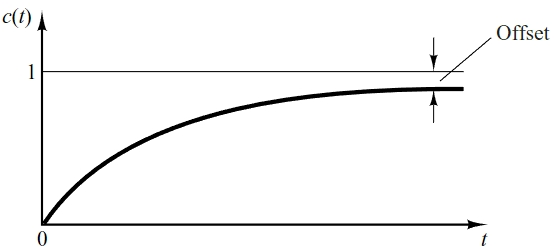
\includegraphics[width=.6\textwidth]{Chapter5/steadystateerrorunitstep.png} %1.png是图片文件的相对路径
    \caption{初始条件为0的情况下输入信号为单位阶跃信号的输出响应} %caption是图片的标题
    \label{steadystateerrorunitstep} %此处的label相当于一个图片的专属标志,目的是方便上下文的引用
\end{figure}

图\ref{steadystateerrorunitstep}所示的是该系统在初始条件为0的情况下输入信号为单位阶跃信号的输出响应,从突出可以看到在$t\rightarrow \infty$时误差信号$e(t)=r(t)-c(t)$不会变为0,这与上述计算分析所得结果相一致。

\begin{figure}
    \centering
    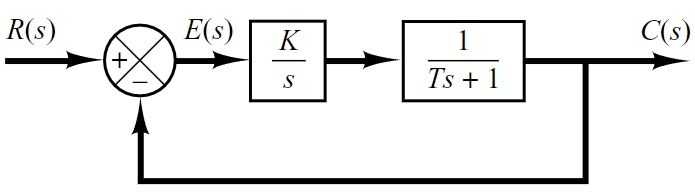
\includegraphics[width=.6\textwidth]{Chapter5/IntegralProportionalControlSystem.png} %1.png是图片文件的相对路径
    \caption{具有积分控制功能的比例控制系统} %caption是图片的标题
    \label{IntegralProportionalControlSystem} %此处的label相当于一个图片的专属标志,目的是方便上下文的引用
\end{figure}

当对图\ref{IntegralProportionalControlSystem}所示系统加入积分控制功能时,以图\ref{IntegralProportionalControlSystem}所示系统为例,假设初始条件为0,输入信号为单位阶跃信号,通过计算可得:
\begin{equation}
    E(s)=\frac{s(Ts+1)}{s(Ts+1)+K}\frac{1}{s}
\end{equation}

根据终值定理可知稳态误差为:
\begin{equation}
    \begin{split}
        e_{ss}&=\lim_{s\rightarrow 0}sE(s)\\
        &=\lim_{s\rightarrow 0}\frac{s^2(Ts+1)}{Ts^2+s+K}\frac{1}{s}\\
        &=0
    \end{split}
\end{equation}

通过上述分析可以发现,加入积分控制功能后,稳态误差$e_{ss}=0$。

\begin{figure}
    \centering
    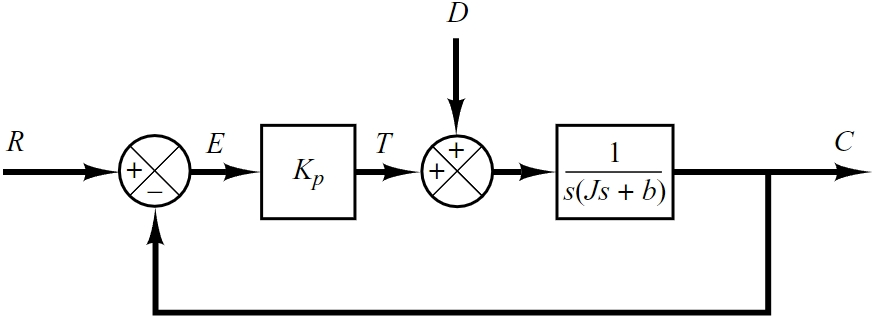
\includegraphics[width=.6\textwidth]{Chapter5/DisturbanceProportionalControlSystem.png} %1.png是图片文件的相对路径
    \caption{扰动存在时的比例控制系统} %caption是图片的标题
    \label{DisturbanceProportionalControlSystem} %此处的label相当于一个图片的专属标志,目的是方便上下文的引用
\end{figure}

当系统中具有扰动时,在比例积分控制系统中会导致额外的有扰动引起的稳态误差,以图\ref{DisturbanceProportionalControlSystem}所示系统为例,假定系统的初始状态为0且扰动为“幅值为$T_d$的阶跃信号”,那么由扰动引起的$E(s)$为(LTI系统中,每个输入对系统的影响是互相独立的。假定其他输入都为0,此时系统的各个节点的输出只由不为0的那个输入决定,能更加便捷的求出不为0的那个输入对节点的影响):
\begin{equation}
    E_D(s)=-\frac{1}{Js^2+bs+K_p}D(s)
\end{equation}

根据终值定理可知由扰动引起的稳态误差为:
\begin{equation}
    \begin{split}
        e_{ss\_D}&=\lim_{s\rightarrow 0}sE(s)\\
        &=\lim_{s\rightarrow 0}\frac{-s}{Js^2+bs+K_p}\frac{T_d}{s}\\
        &=-\frac{T_d}{K_p}
    \end{split}
\end{equation}

所以由扰动信号$d(t)$引起的稳态误差在比例控制系统中不为0。

\begin{figure}
    \centering
    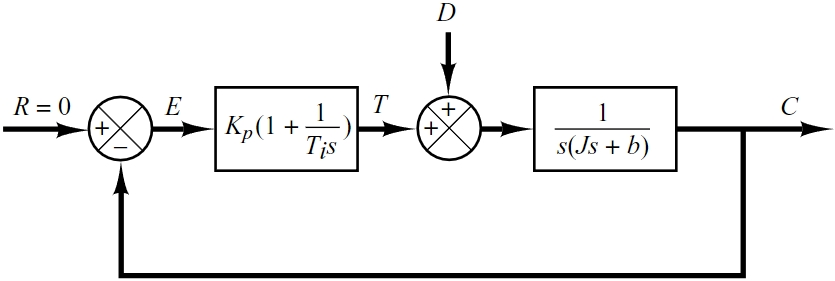
\includegraphics[width=.6\textwidth]{Chapter5/IntegralDisturbanceProportionalControlSystem.png} %1.png是图片文件的相对路径
    \caption{扰动存在时具有积分控制功能的比例控制系统} %caption是图片的标题
    \label{IntegralDisturbanceProportionalControlSystem} %此处的label相当于一个图片的专属标志,目的是方便上下文的引用
\end{figure}

当对图\ref{DisturbanceProportionalControlSystem}所示系统加入积分控制功能时,以图\ref{IntegralDisturbanceProportionalControlSystem}所示系统为例,假定系统的初始状态为0且扰动为“幅值为$T_d$的阶跃信号”,那么由扰动引起的$E(s)$为:
\begin{equation}
    E_D(s)=-\frac{s}{Js^3+bs^2+K_ps+\frac{K_p}{T_i}}D(s)
\end{equation}

根据终值定理可知由扰动引起的稳态误差为:
\begin{equation}
    \begin{split}
        e_{ss\_D}&=\lim_{s\rightarrow 0}sE(s)\\
        &=\lim_{s\rightarrow 0}\frac{-s^2}{Js^3+bs^2+K_ps+\frac{K_p}{T_i}}\frac{T_d}{s}\\
        &=0
    \end{split}
\end{equation}

通过上述分析可以发现,加入积分控制功能后,稳态误差$e_{ss\_D}=0$。

\begin{formal}
    微分控制行为对系统性能的影响:微分控制行为可以预测始能误差信号并及时做出修正,从而提高系统的稳定性。
\end{formal}

\begin{figure}
    \centering
    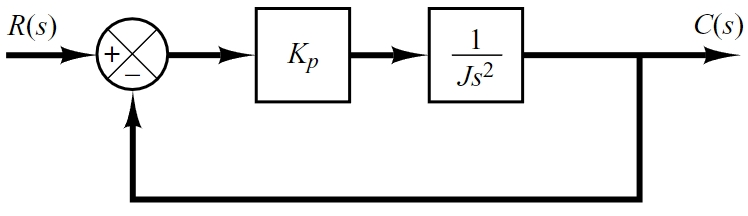
\includegraphics[width=.6\textwidth]{Chapter5/DerivativeProportionalControlSystem.png} %1.png是图片文件的相对路径
    \caption{比例控制系统} %caption是图片的标题
    \label{DerivativeProportionalControlSystem} %此处的label相当于一个图片的专属标志,目的是方便上下文的引用
\end{figure}

以图\ref{DerivativeProportionalControlSystem}所示系统为例,假设初始条件为0,输入信号为单位阶跃信号,当系统中只具有比例控制功能而不具备微分控制功能时,该系统的传输函数为:
\begin{equation}
    \frac{C(s)}{R(s)}=\frac{K_p}{Js^2+K_p}
\end{equation}

根据劳斯稳定性判据可知该系统一定不稳定,即输出一定会振荡。

\begin{figure}
    \centering
    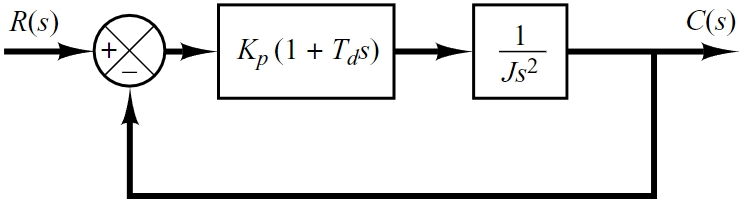
\includegraphics[width=.6\textwidth]{Chapter5/DerivativeProportionalControlSystem2.png} %1.png是图片文件的相对路径
    \caption{具有微分功能的比例控制系统} %caption是图片的标题
    \label{DerivativeProportionalControlSystem2} %此处的label相当于一个图片的专属标志,目的是方便上下文的引用
\end{figure}

当在系统中加入微分控制功能时,以图\ref{DerivativeProportionalControlSystem2}所示系统为例,假设初始条件为0,输入信号为单位阶跃信号,该系统的传输函数为:
\begin{equation}
    \frac{C(s)}{R(s)}=\frac{K_p(1+T_ds)}{Js^2+K_pT_ds+K_p}
\end{equation}

\begin{figure}
    \centering
    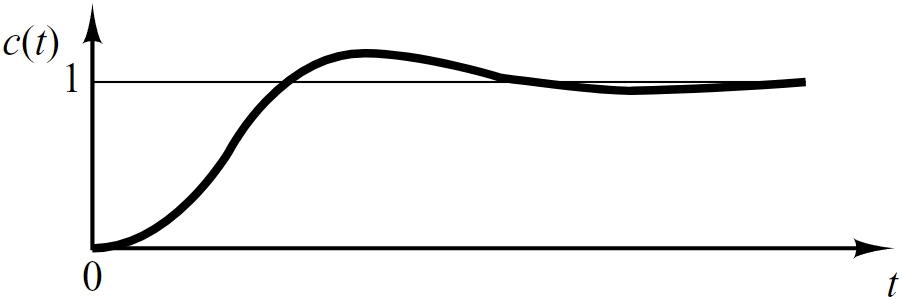
\includegraphics[width=.6\textwidth]{Chapter5/OutputDerivativeProportionalControlSystem2.png} %1.png是图片文件的相对路径
    \caption{零初始条件输入信号为单位阶跃信号具有微分功能的比例控制系统可能的输出曲线} %caption是图片的标题
    \label{OutputDerivativeProportionalControlSystem2} %此处的label相当于一个图片的专属标志,目的是方便上下文的引用
\end{figure}

根据上述劳斯稳定性判据可以确定使得系统稳定的各项参数的取值范围。如果系统是稳定的,根据前文对二阶系统的分析可知,该系统将会具有阻尼性(取值不同,阻尼的状态不同,可能是欠阻尼、临界阻尼或过阻尼),可能的输出如图\ref{OutputDerivativeProportionalControlSystem2}所示,从图中可以看出,加入微分控制功能后,系统最终会趋于稳定。

\subsection{单位反馈控制系统的稳态误差}
任何一个单位负反馈控制系统针对某一种或几种类型的输入都有可能会产生稳态误差,具体哪些类型的输入信号会产生稳态误差的判断则是可以通过该单位负反馈控制系统的开环传输函数的类型得到。

\begin{formal}
    控制系统分类
\end{formal}

以图\ref{UnitFeedbackControlSystem}所示系统为例,对于任意一个单位负反馈控制系统而言的其开环传输函数$G(s)$都可以改写为:
\begin{equation}
    G(s)=\frac{K(T_as+1)(T_bs+1)...(T_ms+1)}{s^N(T_1s+1)(T_2s+1)...(T_ps+1)}
\end{equation}

其中,如图\ref{UnitFeedbackControlSystem}所示,$G(s)$是组成该单位负反馈控制系统的前馈路径上的一个子系统,我们称系统$G(s)$为$Type$ $N$系统。

\begin{figure}
    \centering
    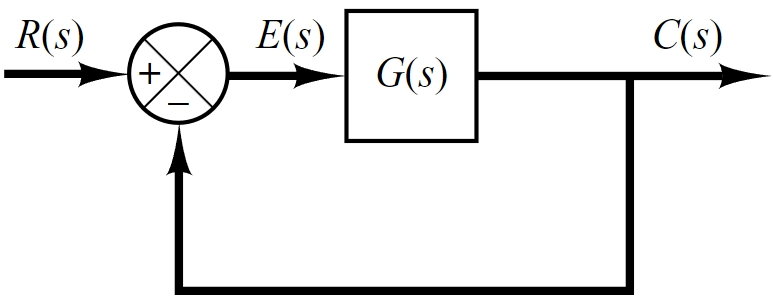
\includegraphics[width=.6\textwidth]{Chapter5/UnitFeedbackControlSystem.png} %1.png是图片文件的相对路径
    \caption{单位反馈控制系统} %caption是图片的标题
    \label{UnitFeedbackControlSystem} %此处的label相当于一个图片的专属标志,目的是方便上下文的引用
\end{figure}

当初始条件为0时易求得$E(s)$为:
\begin{equation}
    E(s)=\frac{1}{1+G(s)}R(s)
\end{equation}

根据终值定理可知稳态误差$e_{ss}$为:
\begin{equation}
    \begin{split}
        e_{ss}&=\lim_{t\rightarrow \infty}e(t)\\
        &=\lim_{s\rightarrow 0}sE(s)\\
        &=\lim_{s\rightarrow 0}\frac{sR(s)}{1+G(s)}\\
        &=\lim_{s\rightarrow 0}\frac{1}{\frac{1}{sR(s)}+\frac{1}{sR(s)}G(s)}\\
        &=\frac{1}{\lim_{s\rightarrow 0}\frac{1}{sR(s)}+\lim_{s\rightarrow 0}\frac{1}{sR(s)}G(s)}
    \end{split}
\end{equation}

所以该单位负反馈系统的稳态误差由$\lim_{s\rightarrow 0}\frac{1}{sR(s)}+\lim_{s\rightarrow 0}\frac{1}{sR(s)}G(s)$所决定的,具体而言:
\begin{itemize}
    \item 当$\lim_{s\rightarrow 0}\frac{1}{sR(s)}+\lim_{s\rightarrow 0}\frac{1}{sR(s)}G(s)=0$时,该单位负反馈系统的稳态误差$e_{ss}=\infty$。
    \item 当$\lim_{s\rightarrow 0}\frac{1}{sR(s)}+\lim_{s\rightarrow 0}\frac{1}{sR(s)}G(s)=K$时(K为非零非无穷的有限值),该单位负反馈系统的稳态误差$e_{ss}=\frac{1}{K}$。
    \item 当$\lim_{s\rightarrow 0}\frac{1}{sR(s)}+\lim_{s\rightarrow 0}\frac{1}{sR(s)}G(s)=\infty$时,该单位负反馈系统的稳态误差$e_{ss}=0$。
\end{itemize}

尽管单位负反馈系统输入信号的类型有无穷多种可能,但绝大多数情况下单位负反馈系统的输入信号为阶跃信号、斜坡信号和双曲函数信号这三种,因此在判断单位负反馈系统对输入信号的跟随能力时一般会根据当输入信号是这三种信号的稳态误差进行判断。
\begin{formal}
    当输入信号是因果阶跃信号时(静态位移误差常数$K_p$)
\end{formal}

    由于$r(t)=A·\epsilon(t)$(其中A为常数),所以$R(s)=\frac{A}{s}$,即$sR(s)=A$,因此可得:
    \begin{equation}
        \begin{split}
            &\lim_{s\rightarrow 0}\frac{1}{sR(s)}+\lim_{s\rightarrow 0}\frac{1}{sR(s)}G(s)\\
            =&\frac{1}{A}+\frac{1}{A}\lim_{s\rightarrow 0}G(s)\\
            =&\frac{1}{A}(1+\lim_{s\rightarrow 0}G(s))
        \end{split}
    \end{equation}
    
    定义静态位移误差常数$K_p$为:$K_p=\lim_{s\rightarrow 0}G(s)=G(0)$,上式可以改写为:
    \begin{equation}
        \lim_{s\rightarrow 0}\frac{1}{sR(s)}+\lim_{s\rightarrow 0}\frac{1}{sR(s)}G(s)=\frac{1}{A}(1+K_p)
    \end{equation}

    即:
    \begin{equation}
        \begin{split}
            e_{ss}&=\frac{1}{\lim_{s\rightarrow 0}\frac{1}{sR(s)}+\lim_{s\rightarrow 0}\frac{1}{sR(s)}G(s)}\\
            &=\frac{A}{1+K_p}
        \end{split}
    \end{equation}

    因此对于给定的因果阶跃信号而言,其稳态误差$e_{ss}$取决于静态位移误差常数$K_p$。也就是说我们可以通过静态位移误差常数$K_p=\lim_{s\rightarrow 0}G(s)=G(0)$判断“单位负反馈系统对因果阶跃信号的跟随能力”。

    由于系统的传输函数$G(s)$可以改写为:$G(s)=\frac{K(T_as+1)(T_bs+1)...(T_ms+1)}{s^N(T_1s+1)(T_2s+1)...(T_ps+1)}$,所以:
    
    (1)$N=0$,即子系统$G(s)$为$Type$ $0$系统时,静态位移误差常数为:
    \begin{equation}
        K_p=\lim_{s\rightarrow 0}\frac{K(T_as+1)(T_bs+1)...}{(T_1s+1)(T_2s+1)...}=K
    \end{equation}
    
    (2)$N>0$,即子系统$G(s)$为$Type$ $1$或更高的系统时,静态位移误差常数为:
    \begin{equation}
        K_p=\lim_{s\rightarrow 0}\frac{K(T_as+1)(T_bs+1)...}{s^N(T_1s+1)(T_2s+1)...}=\infty
    \end{equation}
    
    因此对于$Type$ $0$系统而言,静态位移误差常数为有限值,对于$Type$ $1$或更高的系统而言,静态位移误差常数为无穷大值。

    所以当输入为因果阶跃信号$r(t)=A·\epsilon(t)$(其中A为常数)时,稳态误差$e_{ss}$为:
\begin{equation}
    \begin{split}
        e_{ss}&=\frac{A}{1+K},\quad for\_type\_0\_systems\\
        e_{ss}&=0,\quad for\_type\_1\_or\_higher\_systems\\
    \end{split}
\end{equation}

综上所述,对于$G(s)$为$Type$ $0$的单位负反馈系统而言,其可以跟随因果阶跃信号,但是会存在一定的误差;对于$G(s)$为$Type$ $1$或更高的单位负反馈系统而言,其可以完全跟随因果阶跃信号,不存在误差。

\begin{formal}
    当输入信号是因果斜坡信号时(静态速度误差常数$K_v$)
\end{formal}

由于因果斜坡信号$r(t)=A·t\epsilon(t)$(其中A为常数),所以$R(s)=\frac{A}{s^2}$,即$sR(s)=\frac{A}{s}$,因此可得:
\begin{equation}
    \begin{split}
        &\lim_{s\rightarrow 0}\frac{1}{sR(s)}+\lim_{s\rightarrow 0}\frac{1}{sR(s)}G(s)\\
        =&\lim_{s\rightarrow 0}\frac{s}{A}+\frac{1}{A}\lim_{s\rightarrow 0}sG(s)\\
        =&0+\frac{1}{A}\lim_{s\rightarrow 0}sG(s)\\
        =&\frac{1}{A}\lim_{s\rightarrow 0}sG(s)
    \end{split}
\end{equation}

定义静态速度误差常数$K_v$为:$K_v=\lim_{s\rightarrow 0}sG(s)$,上式可以改写为:
\begin{equation}
    \lim_{s\rightarrow 0}\frac{1}{sR(s)}+\lim_{s\rightarrow 0}\frac{1}{sR(s)}G(s)=\frac{1}{A}K_v
\end{equation}

即:
\begin{equation}
    \begin{split}
        e_{ss}&=\frac{1}{\lim_{s\rightarrow 0}\frac{1}{sR(s)}+\lim_{s\rightarrow 0}\frac{1}{sR(s)}G(s)}\\
        &=\frac{A}{K_v}
    \end{split}
\end{equation}

因此对于给定的因果斜坡信号而言,其稳态误差$e_{ss}$取决于静态速度误差常数$K_v$。也就是说我们可以通过静态位移误差常数$K_v=\lim_{s\rightarrow 0}sG(s)$判断“单位负反馈系统对因果斜坡信号的跟随能力”。

由于系统的传输函数$G(s)$可以改写为:$G(s)=\frac{K(T_as+1)(T_bs+1)...(T_ms+1)}{s^N(T_1s+1)(T_2s+1)...(T_ps+1)}$,所以:

所以对于子系统$G(s)$为$Type$ $0$的单位负反馈系统而言:
\begin{equation}
    K_v=\lim_{s\rightarrow 0}\frac{sK(T_as+1)(T_bs+1)...}{(T_1s+1)(T_2s+1)...}=0
\end{equation}

所以对于子系统$G(s)$为$Type$ $1$的单位负反馈系统而言:
\begin{equation}
    K_v=\lim_{s\rightarrow 0}\frac{sK(T_as+1)(T_bs+1)...}{s(T_1s+1)(T_2s+1)...}=K
\end{equation}

所以对于子系统$G(s)$为$Type$ $2$或更高的单位负反馈系统而言:
\begin{equation}
    K_v=\lim_{s\rightarrow 0}\frac{sK(T_as+1)(T_bs+1)...}{s^N(T_1s+1)(T_2s+1)...}=\infty
\end{equation}

因此对于不同$G(s)$类型的单位负反馈系统的稳态误差为:
\begin{equation}
    \begin{split}
        e_{ss}&=\frac{1}{K_v}=\infty,\quad for\_type\_0\_systems\\
        e_{ss}&=\frac{1}{K_v}=\frac{1}{K},\quad for\_type\_1\_systems\\
        e_{ss}&=0,\quad for\_type\_2\_or\_higher\_systems
    \end{split}
\end{equation}

\begin{figure}
    \centering
    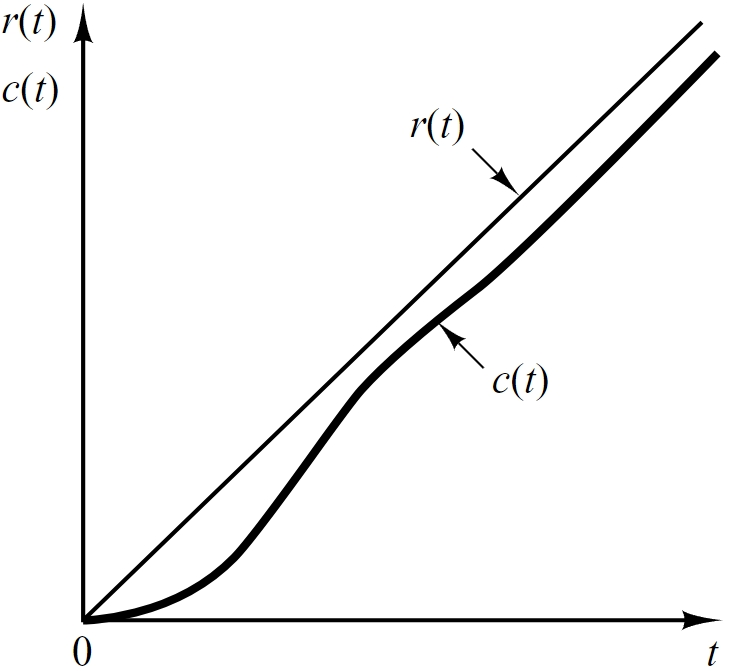
\includegraphics[width=.4\textwidth]{Chapter5/unitramptype1.png} %1.png是图片文件的相对路径
    \caption{零初始条件输入信号为单位斜坡信号的输出曲线} %caption是图片的标题
    \label{unitramptype1} %此处的label相当于一个图片的专属标志,目的是方便上下文的引用
\end{figure}

通过分析发现,$G(s)$为$Type$ $0$的单位负反馈系统的输出无法跟随单位斜坡输入信号变化;$G(s)$为$Type$ $1$的单位负反馈系统的输出可以跟随单位斜坡输入信号变化,但是存在误差,如图\ref{unitramptype1}所示;$G(s)$为$Type$ $2$或更高的单位负反馈系统的输出可以跟随单位斜坡输入信号变化,且不存在误差。

\begin{formal}
    当输入信号是因果双曲信号时(静态加速度误差常数$K_a$)
\end{formal}
由于因果双曲信号$r(t)=A·\frac{t^2}{2}\epsilon(t)$(其中A为常数),所以$R(s)=\frac{A}{s^3}$,即$sR(s)=\frac{A}{s^2}$,因此可得:
\begin{equation}
    \begin{split}
        &\lim_{s\rightarrow 0}\frac{1}{sR(s)}+\lim_{s\rightarrow 0}\frac{1}{sR(s)}G(s)\\
        =&\lim_{s\rightarrow 0}\frac{s^2}{A}+\frac{1}{A}\lim_{s\rightarrow 0}s^2G(s)\\
        =&0+\frac{1}{A}\lim_{s\rightarrow 0}s^2G(s)\\
        =&\frac{1}{A}\lim_{s\rightarrow 0}s^2G(s)
    \end{split}
\end{equation}

定义静态速度误差常数$K_a$为:$K_a=\lim_{s\rightarrow 0}s^2G(s)$,上式可以改写为:
\begin{equation}
    \lim_{s\rightarrow 0}\frac{1}{sR(s)}+\lim_{s\rightarrow 0}\frac{1}{sR(s)}G(s)=\frac{1}{A}K_a
\end{equation}

即:
\begin{equation}
    \begin{split}
        e_{ss}&=\frac{1}{\lim_{s\rightarrow 0}\frac{1}{sR(s)}+\lim_{s\rightarrow 0}\frac{1}{sR(s)}G(s)}\\
        &=\frac{A}{K_a}
    \end{split}
\end{equation}

因此对于给定的因果双曲信号而言,其稳态误差$e_{ss}$取决于静态加速度误差常数$K_a$。也就是说我们可以通过静态加速度误差常数$K_a=\lim_{s\rightarrow 0}s^2G(s)$判断“单位负反馈系统对因果双曲信号的跟随能力”。

由于系统的传输函数$G(s)$可以改写为:$G(s)=\frac{K(T_as+1)(T_bs+1)...(T_ms+1)}{s^N(T_1s+1)(T_2s+1)...(T_ps+1)}$,所以:

所以对于子系统$G(s)$为$Type$ $0$单位负反馈系统而言:
\begin{equation}
    K_a=\lim_{s\rightarrow 0}\frac{s^2K(T_as+1)(T_bs+1)...}{(T_1s+1)(T_2s+1)...}=0
\end{equation}

所以对于子系统$G(s)$为$Type$ $1$单位负反馈系统而言:
\begin{equation}
    K_a=\lim_{s\rightarrow 0}\frac{s^2K(T_as+1)(T_bs+1)...}{s(T_1s+1)(T_2s+1)...}=0
\end{equation}

所以对于子系统$G(s)$为$Type$ $2$的单位负反馈系统而言:
\begin{equation}
    K_a=\lim_{s\rightarrow 0}\frac{s^2K(T_as+1)(T_bs+1)...}{s^2(T_1s+1)(T_2s+1)...}=K
\end{equation}

所以对于子系统$G(s)$为$Type$ $3$或更高的单位负反馈系统而言:
\begin{equation}
    K_a=\lim_{s\rightarrow 0}\frac{s^2K(T_as+1)(T_bs+1)...}{s^N(T_1s+1)(T_2s+1)...}=\infty
\end{equation}

因此对于$G(s)$不同类型的单位负反馈系统的稳态误差为:
\begin{equation}
    \begin{split}
        e_{ss}&=\frac{1}{K_a}=\infty,\quad for\_type\_0\_and\_type\_1\_systems\\
        e_{ss}&=\frac{1}{K_a}=\frac{1}{K},\quad for\_type\_2\_systems\\
        e_{ss}&=0,\quad for\_type\_3\_or\_higher\_systems
    \end{split}
\end{equation}

\begin{figure}
    \centering
    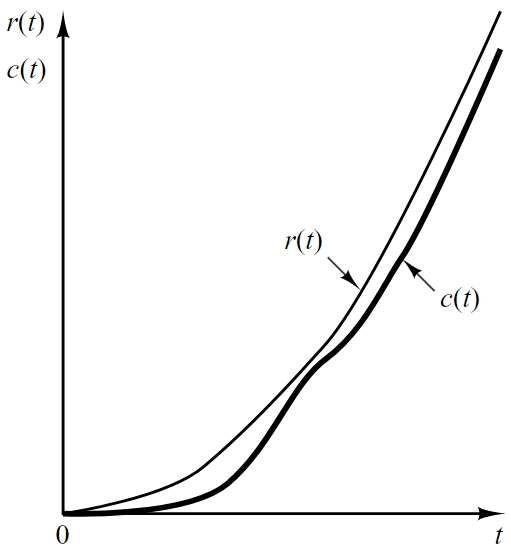
\includegraphics[width=.4\textwidth]{Chapter5/unitparabolictype2.png} %1.png是图片文件的相对路径
    \caption{零初始条件输入信号为单位双曲信号的输出曲线} %caption是图片的标题
    \label{unitparabolictype2} %此处的label相当于一个图片的专属标志,目的是方便上下文的引用
\end{figure}

通过分析发现,$G(s)$为$Type$ $0$和$1$的单位负反馈系统的输出无法跟随单位斜坡输入信号变化;$G(s)$为$Type$ $2$的单位负反馈系统的输出可以跟随单位斜坡输入信号变化,但是存在误差,如图\ref{unitparabolictype2}所示;$G(s)$为$Type$ $3$或更高的单位负反馈系统的输出可以跟随单位斜坡输入信号变化,且不存在误差。

\begin{formal}
    误差常数总结
\end{formal}
对于任意一个系统$G(s)$而言,我们可以将其接为“单位增益负反馈”的形式,通过静态位移误差常数$K_p$、静态速度误差常数$K_v$和静态加速度误差常数$K_a$分别判断该由$G(s)$所构成的“单位增益负反馈”系统对因果阶跃信号、因果斜坡信号和因果双曲信号的跟随能力。其中,相应静态误差常数越大,对相应信号的跟随能力越强,对于相应信号的稳态误差越小。

虽然由任意$G(s)$所构成的“单位增益负反馈”系统有无穷多种,但并非每个由任意$G(s)$所构成的“单位增益负反馈”系统的误差常数结果都是不同的。通过将$G(s)$根据$N$-type进行分类讨论后可以进一步推得二级结论:图\ref{Steady-StateError}所示的是$G(s)$属于不同type系统情况下在不同输入信号情况时由该$G(s)$所构成的“单位增益负反馈”系统的稳态误差的总结,从中可以看出,有限值形式的稳态误差存在于对角线处,对角线上方的稳态误差为无穷大,对角线下方的稳态误差为0。其中有限值形式的稳态误差表明在时间无穷大即瞬态响应耗尽时,输出的变化速率将和输入的变化速率相同,只不过会存在一个差值。

通过这个二级结论我们可以进一步发现:
\begin{itemize}
    \item 如果我们明确子系统$G(s)$的传输函数,那么我们就可以直接判断子系统$G(s)$的type类型,从而根据图\ref{Steady-StateError}直接判断由这个$G(s)$所构成的“单位增益负反馈”系统对不同信号的跟随能力。
    \item 如果我们不知道一个子系统$G(s)$的传输函数,那么我们可以通过测试由这个子系统$G(s)$所构成的“单位增益负反馈”系统的$K_p$、$K_v$和$K_a$从而判断子系统$G(s)$的type类型。
\end{itemize}

\begin{figure}
    \centering
    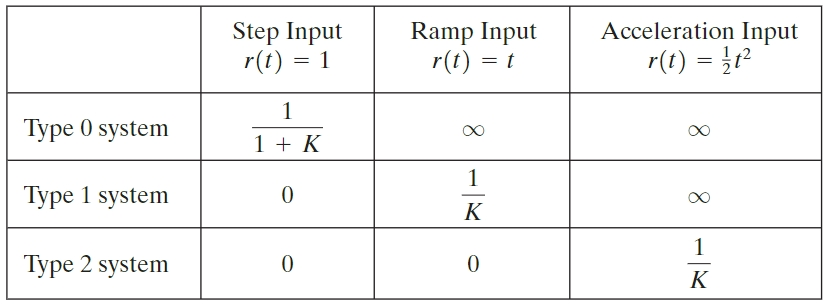
\includegraphics[width=.6\textwidth]{Chapter5/Steady-StateError.png} %1.png是图片文件的相对路径
    \caption{上述系统在不同输入信号情况下的稳态误差} %caption是图片的标题
    \label{Steady-StateError} %此处的label相当于一个图片的专属标志,目的是方便上下文的引用
\end{figure}

之所以称三个静态误差常数分别为“位移”、“速度”、“加速度”是因为在定义时他们三个量之间的“形式上”满足导数关系,这一点从拉普拉斯变换的微积分特性可以看出。但这并不代表他们的单位是导数关系,从这三个量的基本定义也可以看出,这三个量的维度(一般为单位)和输入输出信号是相同的,所以在单位上这三个量是一致的。

\newpage

\section{控制系统分析及基于根轨迹法的系统设计}
\subsection{傅里叶级数、傅里叶变换和拉普拉斯变换回顾}
\begin{formal}
    傅里叶级数
\end{formal}

假设$\phi_1(t),\phi_2(t)...\phi_n(t)$在$(t_1,t_2)$之间构成完备正交函数集,则在$(t_1,t_2)$区间内函数$f(t)$可以写为:$f(t)=C_1\phi_1(t)+C_2\phi_2(t)+...+C_n\phi_i(t)$。其中:$C_i=\frac{\int_{t_1}^{t_2}f(t)\phi^*_i(t)dt}{\int_{t_1}^{t_2}\phi_i(t)\phi^*_i(t)dt}=\frac{1}{K_i}\int_{t_1}^{t_2}f(t)\phi^*_i(t)dt$

两组典型的在区间$(t_0,t_0+T)$上的完备正交函数集:

(1)三角函数集{$1,cos(n\Omega t),sin(n\Omega t),n=1,2,3...$}

(2)虚指数函数集{$e^{jn\Omega t},n=0,\pm1,\pm2,...$ }

其中$T$和$\Omega$的关系为$\Omega=\frac{2\pi}{T}$.

若$f(t)$为周期信号,周期为$T$,角频率为$\Omega=\frac{2\pi}{T}$,且函数满足狄里赫利条件:
\begin{Definition}{狄里赫利条件}{}
    \begin{itemize}
        \item 在一周期内,连续或只有有限个第一类间断点;
        \item 在一周期内,极大值和极小值的数目应是有限个;
        \item 在一周期内,信号是绝对可积的。
    \end{itemize}
\end{Definition}

则在$(t_0,t_0+T)$中有:
\begin{equation}
    \begin{split}
        f(t)&=\frac{a_0}{2}+\sum_{n = 1}^{\infty} a_ncos(n\Omega t)+ \sum_{n = 1}^{\infty} b_nsin(n\Omega t)\\
        &=\frac{a_0}{2}+\sum_{n = 1}^{\infty}\sqrt{a_n^2+b_n^2}(\frac{a_n}{\sqrt{a_n^2+b_n^2}}cos(n\Omega t)+\frac{b_n}{\sqrt{a_n^2+b_n^2}}sin(n\Omega t))
    \end{split}
\end{equation}

其中$a_n=\frac{2}{T}\int_{\frac{-T}{2}}^{\frac{T}{2}}f(t)cos(n\Omega t)dt$,$b_n=\frac{2}{T}\int_{\frac{-T}{2}}^{\frac{T}{2}}f(t)sin(n\Omega t)dt$。

令$A_n=\sqrt{a_n^2+b_n^2}$,$cos(\phi_n)=\frac{a_n}{\sqrt{a_n^2+b_n^2}}=\frac{a_n}{A_n}$,$sin(\phi_n)=\frac{-b_n}{\sqrt{a_n^2+b_n^2}}=\frac{-b_n}{A_n}$,则上式可以写为:
\begin{equation}
    \begin{split}
        f(t)&=\frac{a_0}{2}+\sum_{n = 1}^{\infty}A_n[cos(\phi_n)cos(n\Omega t)-sin(\phi_n)sin(n\Omega t)]\\
        &=\frac{a_0}{2}+\sum_{n = 1}^{\infty}A_ncos(n\Omega t+\phi_n)
    \end{split}
\end{equation}

由于$b_0=0$,所以$a_0=A_0cos(\phi_0)$,其中$A_0=|a_0|$,则上式可以写为:
\begin{equation}
    \begin{split}
        f(t)&=\frac{A_0}{2}cos(\phi_0)+\sum_{n = 1}^{\infty}A_ncos(n\Omega t+\phi_n)\\
        &=\frac{A_0}{2}cos(\phi_0)+\sum_{n = 1}^{\infty}\frac{A_n}{2}[e^{j(n\Omega t+\phi_n)}+e^{-j(n\Omega t+\phi_n)}]\\
        &=\frac{A_0}{2}cos(\phi_0)+\frac{1}{2}\sum_{n = 1}^{\infty}A_ne^{j\phi_n}e^{jn\Omega t}+\frac{1}{2}\sum_{n = 1}^{\infty}A_ne^{-j\phi_n}e^{-jn\Omega t}
    \end{split}
\end{equation}

其中,由于$a_0$为常数,所以$\phi_0=k\pi$($k$为常数),即$e^{j\phi_0}e^{j0\Omega t}=cos(0\Omega t+\phi_0)=cos(\phi_0)$。所以当$a_n$,$b_n$,$A_n$,$\phi_n$在无论n取何值均满足上述表达式时,则上式可以写为(如果$a_n$,$b_n$,$A_n$,$\phi_n$只在$n≥0$满足上述表达式时,则得不到下述推导):
\begin{equation}
    \begin{split}
        f(t)&=\frac{A_0}{2}cos(\phi_0)+\frac{1}{2}\sum_{n = 1}^{\infty}A_ne^{j\phi_n}e^{jn\Omega t}+\frac{1}{2}\sum_{n = -\infty}^{-1}A_ne^{j\phi_n}e^{jn\Omega t}\\
        &=\frac{1}{2}A_0e^{j\phi_0}e^{j0\Omega t}+\frac{1}{2}\sum_{n = 1}^{\infty}A_ne^{j\phi_n}e^{jn\Omega t}+\frac{1}{2}\sum_{n = -\infty}^{-1}A_ne^{j\phi_n}e^{jn\Omega t}\\
        &=\frac{1}{2}\sum_{n = -\infty}^{\infty}A_ne^{j\phi_n}e^{jn\Omega t}
    \end{split}
\end{equation}

令$F_n=\frac{1}{2}A_ne^{j\phi_n}$,称$F_n$为傅里叶系数,则上式可以写为:
\begin{equation}
    f(t)=\sum_{n = -\infty}^{\infty}F_ne^{jn\Omega t}
\end{equation}

其中$F_n$为:
\begin{equation}
    \begin{split}
        F_n&=\frac{1}{2}A_ne^{j\phi_n}\\
        &=\frac{1}{2}(A_ncos(\phi_n)+jA_nsin(\phi_n))\\
        &=\frac{1}{2}(a_n-jb_n)\\
        &=\frac{1}{T}\int_{-\frac{T}{2}}^{\frac{T}{2}}f(t)cos(n\Omega t)dt-j\frac{1}{T}\int_{-\frac{T}{2}}^{\frac{T}{2}}f(t)sin(n\Omega t)dt\\
        &=\frac{1}{T}\int_{-\frac{T}{2}}^{\frac{T}{2}}f(t)e^{-jn\Omega t}dt
    \end{split}
\end{equation}

从上述分析中可以看出,当一个周期信号满足狄里赫利条件时,在区间$(t_0,t_0+T)$中函数f(t)是“直流分量”、“一次谐波分量”、“二次谐波分量”...“n次谐波分量”...的线性组合,其中$A_n$为“n次谐波分量”(角频率为$n\Omega$的余弦函数)的幅值,$\phi_n$为“n次谐波分量”的相位。

因为傅里叶系数$F_n$的定义为:$F_n=\frac{1}{2}A_ne^{j\phi_n}$,所以傅里叶系数$F_n$包含了“n次谐波分量”的幅值以及相位的信息。其中“n次谐波分量”的幅值=$A_n$=$2|F_n|$,“n次谐波分量”的相位=$\phi_n$。

由于$e^{j\phi_n}=cos(\phi_n)+jsin(\phi_n)$且$F_n=\frac{1}{2}A_ne^{j\phi_n}$,所以从向量的角度看,在复平面上$e^{j\phi_n}$对应的就是以$F_n$的方向为方向的单位向量,所以$\phi_n$也就等于$F_n$的方向(从原点出发指向$F_n$点的箭头方向)在逆时针下与正实轴的夹角$\theta $。

\begin{formal}
    傅里叶变换
\end{formal}

当周期$T\rightarrow \infty$时,满足狄里赫利条件的周期信号退化为满足狄里赫利条件的非周期信号,该信号的傅里叶系数$Fn\rightarrow 0$,谱线间隔$\Omega \rightarrow 0$,离散频谱变为连续频谱。

尽管组成满足狄里赫利条件的非周期信号($T\rightarrow \infty$的满足狄里赫利条件的周期信号)的各次谐波分量的幅值都特别小,但是仍然存在有差别,因此引入频谱密度函数$F(j\omega)$,$F(j\omega)$也称为信号$f(t)$的傅里叶变换。

频谱密度函数$F(j\omega)$定义为:
\begin{equation}
    \begin{split}
        F(j\omega)&=\lim_{T \to \infty} \frac{F_n}{1/T}\\
        &=\lim_{T \to \infty} F_nT\\
        &=\lim_{T \to \infty}\int_{\frac{-T}{2}}^{\frac{T}{2}}f(t)e^{-jn\Omega t}dt\\
        &=\int_{-\infty}^{\infty}f(t)e^{-j\omega t}dt
    \end{split}
\end{equation}

根据频谱密度函数的定义可得满足狄里赫利条件的非周期信号($T\rightarrow \infty$的满足狄里赫利条件的周期信号)可以表示为:
\begin{equation}
    \begin{split}
        f(t)&=\sum_{n=-\infty}^{\infty}F_ne^{jn\Omega t}\\
        &=\sum_{n=-\infty}^{\infty}TF_ne^{jn\Omega t}\frac{1}{T}\\
        &=\sum_{n=-\infty}^{\infty}F(j\omega)e^{j\omega t}\frac{d\omega}{2\pi}\\
        &=\frac{1}{2\pi}\int_{-\infty}^{\infty}F(j\omega)e^{j\omega t}d\omega
    \end{split}
\end{equation}

其中我们称$F(j\omega)=\int_{-\infty}^{\infty}f(t)e^{-j\omega t}dt$为傅里叶变换,称$f(t)=\frac{1}{2\pi}\int_{-\infty}^{\infty}F(j\omega)e^{j\omega t}d\omega$为傅里叶逆变换。

根据频谱密度函数$F(j\omega)$的定义可知,$F(j\omega)$相较于傅里叶系数$F_n$的区别在于乘以了一个无穷大的常数,因此频谱密度函数$F(j\omega)$的幅值|$F(j\omega)$|不再像|$F_n$|与谐波分量的幅值直观联系(幅值=$A_n$=$2|F_n|$),但两个不同的满足狄里赫利条件的非周期信号的相同角频率的谐波分量的幅值之比等于$\frac{|F_{1n}|}{|F_{2n}|}=\frac{|F_{1n}T|}{|F_{2n}T|}=\frac{|F_1(j\omega)|}{|F_2(j\omega)|}$,即傅里叶变换$F(j\omega)$可以直接用其幅值求谐波分量的幅值比。

此外,由于$F(j\omega)$相较于傅里叶系数$F_n$的区别只在于乘以了一个无穷大的常数,因此$F(j\omega)$在复平面上在逆时针下与正实轴的夹角与$F_n$相同,即傅里叶变换也能够直接用于求解组成满足狄里赫利条件的非周期信号的各角频率谐波分量的相位$\phi_n$。

因此傅里叶变换$F(j\omega)$即可以用于分析幅值比又可以进行相位计算。

例如(正如在最初的分析中所述,满足狄里赫利条件的非周期信号的傅里叶系数$F_n$虽然约为0,但并不是0,因此要求解两个相同频率的谐波信号的幅值比和相位差时,可以通过$\frac{F_{1n}}{F_{2n}}$进行求解):
\begin{equation}
    \begin{split}
        \frac{F_{1n}}{F_{2n}}&=\frac{|F_{1n}|e^{j\phi_1}}{|F_{2n}|e^{j\phi_2}}=\frac{|F_{1n}|}{|F_{2n}|}e^{j(\phi_1-\phi_2)}\\
        &=\frac{T|F_{1n}|e^{j\phi_1}}{T|F_{2n}|e^{j\phi_2}}\\
        &=\frac{|F_1(j\omega)|e^{j\phi_1}}{|F_2(j\omega)|e^{j\phi_2}}\\
        &=\frac{F_1{(j\omega)}}{F_2{(j\omega)}}\label{fuzhi&xiangwei}
    \end{split}
\end{equation}

由于任意一个周期信号都可以看作是一时限非周期信号的周期拓展,即:$f_T(t)=\delta_T(t)*f_0(t)=\sum_{m=-\infty}^{\infty}\delta(t-mT)*f_0(t)$,所以任一周期信号都可以看作是非周期信号的线性组合。

当非周期信号$f_0(t)$满足狄里赫利条件时,每个非周期信号$\delta(t-mT)*f_0(t)$都将满足满足狄里赫利条件,并可以等价表示为无穷多个谐波分量的线性组合,此时所组成的信号$f_T(t)$也可以等价表示为无穷多个谐波分量的线性组合。

如果周期信号$f_T(t)$满足狄里赫利条件,那么相应的$f_0(t)$也将满足狄里赫利条件。因此可得,满足狄里赫利条件的周期信号$f_T(t)$可以被等价表示为无穷多个谐波分量的线性组合。(这与傅里叶级数的推导并不矛盾,因为满足狄里赫利条件的周期信号除了$n\Omega$处的谐波分量外其余谐波分量的幅值均为0,所以在傅里叶级数的表达式中只有$n\Omega$项。)

由于$F_m(j\omega)=\int_{-\infty}^{\infty}\delta(t-mT)*f_0(t)e^{-j\omega t}dt$表示的是$\delta(t-mT)*f_0(t)$的谐波分量的幅值密度和相位,所以$\sum_{m=-\infty}^{\infty}F_m(j\omega)$表示的是$\sum_{m=-\infty}^{\infty}\delta(t-mT)*f_0(t)$的谐波分量的幅值密度和相位。又因为$f_T(t)=\sum_{-\infty}^{\infty}\delta(t-mT)*f_0(t)$,所以$\sum_{m=-\infty}^{\infty}F_m(j\omega)$表示的也是组成满足狄里赫利条件的周期信号$f_T(t)$的谐波分量的幅值密度和相位。(证明过程与后文中广义傅里叶变换部分同理)

由于:
\begin{equation}
    \begin{split}
        \sum_{m=-\infty}^{\infty}F_m(j\omega)&=\sum_{m=-\infty}^{\infty}\int_{-\infty}^{\infty}\delta(t-mT)*f_0(t)e^{-j\omega t}dt\\
        &=\int_{-\infty}^{\infty}\sum_{m=-\infty}^{\infty}\delta(t-mT)*f_0(t)e^{-j\omega t}dt\\
        &=\int_{-\infty}^{\infty}f_T(t)e^{-j\omega t}dt\\
        &=F_T(j\omega)
    \end{split}
\end{equation}

所以$F_T(j\omega)=\int_{-\infty}^{\infty}f_T(t)e^{-j\omega t}dt$的结果表示的是满足狄里赫利条件的周期信号$f_T(t)$的谐波分量幅值密度和相位。

因此傅里叶变换$F(j\omega)=\int_{-\infty}^{\infty}f(t)e^{-j\omega t}dt$中无论满足狄里赫利条件的$f(t)$是周期信号还是非周期信号,$F(j\omega)=\int_{-\infty}^{\infty}f(t)e^{-j\omega t}dt$都反映了$f(t)$的谐波分量的幅值密度和相位。

综上所述,对于满足狄里赫利条件的任意信号$f(t)$而言,都可以进行傅里叶变换$F(j\omega)=\int_{-\infty}^{\infty}f(t)e^{-j\omega t}dt$,并且傅里叶变换$F(j\omega)$表示的是组成$f(t)$的谐波分量的幅值密度和相位信息。

由于$F(j\omega)$得到的是谐波分量的幅值密度和相位信息,因此虽然无法直接用于求解谐波分量的幅值,但是可以用于求解两个信号在相同角频率处的谐波分量的幅值比和相位差。

上述内容证明了满足狄里赫利条件的周期信号$f_T(t)$可以通过傅里叶变换($F(j\omega)=\int_{-\infty}^{\infty}f(t)e^{-j\omega t}dt$)求得其傅里叶变换$F_T(j\omega)$,那么如何通过$F_T(j\omega)$逆变换得到周期信号$f_T(t)$呢?

由于$f_T(t)=\sum_{m=-\infty}^{\infty}\delta(t-mT)*f_0(t)$,所以:
\begin{equation}
    \begin{split}
        f_T(t)&=\sum_{m=-\infty}^{\infty}\delta(t-mT)*f_0(t)\\
        &=\sum_{m=-\infty}^{\infty}\frac{1}{2\pi}\int_{-\infty}^{\infty}F_m(j\omega)e^{j\omega t}d\omega\\
        &=\frac{1}{2\pi}\sum_{m=-\infty}^{\infty}\int_{-\infty}^{\infty}F_m(j\omega)e^{j\omega t}d\omega\\
        &=\frac{1}{2\pi}\int_{-\infty}^{\infty}\sum_{m=-\infty}^{\infty}F_m(j\omega)e^{j\omega t}d\omega\\
        &=\frac{1}{2\pi}\int_{-\infty}^{\infty}F_T(j\omega)e^{j\omega t}d\omega
    \end{split}
\end{equation}

即傅里叶逆变换$f(t)=\frac{1}{2\pi}\int_{-\infty}^{\infty}F(j\omega)e^{j\omega t}d\omega$也是对于满足狄里赫利条件的任意信号$f(t)$都是成立的。

综上所述,对于满足狄里赫利条件的信号$f(t)$而言,其傅里叶变换和傅里叶逆变换为:

傅里叶变换:
\begin{equation}
    F(j\omega)=\int_{-\infty}^{\infty}f(t)e^{-j\omega t}dt
\end{equation}

傅里叶逆变换为:
\begin{equation}
    f(t)=\frac{1}{2\pi}\int_{-\infty}^{\infty}F(j\omega)e^{j\omega t}d\omega
\end{equation}

尽管上述推导是基于信号满足狄里赫利条件得来的,但经过数学分析发现对于非周期信号而言,只要其满足绝对可积条件,就能够进行傅里叶变换,即看作是无穷多个谐波分量的线性组合。

对于周期信号而言,本专业所遇到的基本所有信号或函数基本都能够满足除绝对可积外的狄里赫利条件的要求,因此简化记忆为,只要周期信号满足绝对可积条件,就能够进行傅里叶变换,即看作是无穷多个谐波分量的线性组合。

综上所述,只要一个信号满足绝对可积条件,那么这个信号就能够进行傅里叶变换,就能够看作是无穷多个谐波分量的线性组合。其中傅里叶变换表示的是组成信号的谐波分量的幅值密度和相位。如果要求两谐波分量间的幅值比和相位差,可以通过傅里叶变换之比$\frac{F_1{(j\omega)}}{F_2{(j\omega)}}$求得。

由于满足绝对可积条件的任一信号都能被看作是无穷多个谐波分量的线性组合,因此每一个满足绝对可积条件的信号实际上都能写成傅里叶级数的形式,这一点是显而易见的。

\begin{formal}
    广义傅里叶变换
\end{formal}

上文中我们证明了满足绝对可积条件的信号可以等价看作是无穷多个谐波分量的线性组合,并可以进行傅里叶变换和傅里叶逆变换,那么对于不满足绝对可积条件的信号而言我们是否可以将其也等价看作是无穷多个谐波分量的线性组合并进行傅里叶变换和傅里叶逆变换呢?

对于不满足绝对可积条件的信号$f(t)$而言,我们将该信号逐段截取为满足绝对可积条件的信号$f_m(t)$,其,即$f(t)=\sum_{m=-\infty}^{\infty}f_m(t)$。

由于$f_m(t)$满足绝对可积条件,因此其可以等价表示为无穷多个谐波分量的线性组合,因此$f(t)$也可以看作是无穷多个谐波分量的线性组合。

通过上文的分析可知,对于任意一个信号$f(t)$,无论其是否满足绝对可积,都可以看作是无穷多个谐波分量的线性组合。

因此可以将$f(t)$展开为$f(t)=\sum_{\omega=-\infty}^{\infty}F_\omega e^{j\omega t}$,同理将$f_m(t)$展开为$f_m(t)=\sum_{\omega=-\infty}^{\infty}F_{m\omega}e^{j\omega t}$,由此可得$\sum_{\omega=-\infty}^{\infty}F_\omega e^{j\omega t}=\sum_{m=-\infty}^{\infty}\sum_{\omega=-\infty}^{\infty}F_{m\omega}e^{j\omega t}$,即$F_\omega=\sum_{m=-\infty}^{\infty}F_{m\omega}$,即:
\begin{equation}
    \begin{split}
        \lim_{T\rightarrow \infty}T·F_\omega&=\lim_{T\rightarrow \infty}\sum_{m=-\infty}^{\infty}T·F_{m\omega}\\
        &=\sum_{m=-\infty}^{\infty}F_m(j\omega)
    \end{split}
\end{equation}

其中$F_m(j\omega)=\int_{-\infty}^{\infty}f_m(t)e^{-j\omega t}dt$表示的是$f_m(t)$的谐波分量的幅值密度和相位,$\lim_{T\rightarrow \infty}T·F_\omega$表示的是$f(t)$的谐波分量的幅值密度和相位。

因此$\sum_{m=-\infty}^{\infty}F_m(j\omega)$表示的是不满足绝对可积条件的信号$f(t)$的谐波分量的幅值密度和相位。

由于:
\begin{equation}
    \begin{split}
        \sum_{m=-\infty}^{\infty}F_m(j\omega)&=\sum_{m=-\infty}^{\infty}\int_{-\infty}^{\infty}f_m(t)e^{-j\omega t}dt\\
        &=\int_{-\infty}^{\infty}\sum_{m=-\infty}^{\infty}f_m(t)e^{-j\omega t}dt\\
        &=\int_{-\infty}^{\infty}f(t)e^{-j\omega t}dt\\
        &=F(j\omega)
    \end{split}
\end{equation}

所以$F(j\omega)=\int_{-\infty}^{\infty}f(t)e^{-j\omega t}dt$表示的是不满足绝对可积条件的信号$f(t)$的谐波分量的幅值密度和相位。

因此傅里叶变换$F(j\omega)=\int_{-\infty}^{\infty}f(t)e^{-j\omega t}dt$中的信号$f(t)$无论是否满足绝对可积条件,$F(j\omega)=\int_{-\infty}^{\infty}f(t)e^{-j\omega t}dt$都反映了$f(t)$的谐波分量的幅值密度和相位。

对于不满足绝对可积条件的信号$f(t)$而言,在得到其傅里叶变换$F(j\omega)$后,怎么逆变换回$f(t)$呢?

由于$f_T(t)=\sum_{m=-\infty}^{\infty}f_m(t)$,所以:
\begin{equation}
    \begin{split}
        f_T(t)&=\sum_{m=-\infty}^{\infty}f_m(t)\\
        &=\sum_{m=-\infty}^{\infty}\frac{1}{2\pi}\int_{-\infty}^{\infty}F_m(j\omega)e^{j\omega t}d\omega\\
        &=\frac{1}{2\pi}\sum_{m=-\infty}^{\infty}\int_{-\infty}^{\infty}F_m(j\omega)e^{j\omega t}d\omega\\
        &=\frac{1}{2\pi}\int_{-\infty}^{\infty}\sum_{m=-\infty}^{\infty}F_m(j\omega)e^{j\omega t}d\omega\\
        &=\frac{1}{2\pi}\int_{-\infty}^{\infty}F(j\omega)e^{j\omega t}d\omega
    \end{split}
\end{equation}

因此傅里叶逆变换$f(t)=\frac{1}{2\pi}\int_{-\infty}^{\infty}F(j\omega)e^{j\omega t}d\omega$对于不满足绝对可积的信号$f(t)$也是成立的。

\begin{formal}
    傅里叶变换总结
\end{formal}

综上所述,对于任意一个信号$f(t)$而言,其都可以等价表示为无穷多个谐波分量线性组合的形式,并都可以进行傅里叶变换得到谐波分量的幅值密度和相位信息,也可以通过傅里叶逆变换得到$f(t)$。

但是由于只有当$f(t)$满足绝对可积条件时,其傅里叶变换所得到的数学表达式易于描述与计算分析,而当$f(t)$不满足绝对可积条件时,其傅里叶变换所得到的数学表达式难以描述与计算分析,因此我们通常只会在$f(t)$满足绝对可积条件时对其进行傅里叶变换以进行频域分析,但这并不意味着只有满足绝对可积条件的$f(t)$可以进行通过傅里叶变换以进行频域分析。

傅里叶变换虽然是基于对组成信号的谐波分量(即信号的频域信息)进行分析这一目标推出的,但是它除了具备频域分析的能力外,还具备了“原式与变换式”一一对应的特性,即具备了换域分析的能力。

尽管只有信号的傅里叶变换式可以对组成该信号的谐波分量进行分析,但是能够与该信号实现一一对应的变换式却不止有傅里叶变换式。也就是说,对于不满足绝对可积条件的信号而言,虽然我们没法直接用傅里叶变换式与原式一一对应(因为不满足绝对可积条件的信号的傅里叶变换式难以用数学表达式来描述),但是我们可以用另一种变换式实现与不满足绝对可积条件的信号一一对应。如果这种变换式同时适用于满足绝对可积条件的信号,那么对任意信号这种变换式都可以实现都一一对应从而使得换域分析对于所有信号都适用。

既然满足绝对可积条件的信号的傅里叶变换与其原信号能够实现一一对应,那么如果存在这么一种变换,即先将原信号转化为满足绝对可积条件的变换式1,再将该变换式1通过傅里叶变换转化为变换式2,那么此时变换式1与变换式2将一一对应,如果我们能保证原信号与变换式1也一一对应,就可以实现原信号与变换式2一一对应。

也就是说如果有一种变换包含了上述两种子变换,且能够保证第一种子变换可一一对应,那么这种变换就可以实现任意一个原信号都能与变换式的一一对应,从而实现换域分析对于所有信号都适用。

根据上述分析的思路,推导出了基于傅里叶变换的新变换,我们称该新变换为拉普拉斯变换。

\begin{formal}
    拉普拉斯变换
\end{formal}

当函数f(t)不满足绝对可积条件:$\int_{-\infty}^{\infty}|f(t)|dt<\infty$时,则其傅里叶变换难以用较易的数学表达式进行表述,但如果给$f(t)$乘以一个衰减因子$e^{-\sigma t}$($\sigma$为实常数)构建一个新函数$g(t)=f(t)e^{-\sigma t}$并保证$g(t)$满足绝对可积条件,那么$g(t)$的傅里叶变换为:
\begin{equation}
    \begin{split}
        G(j\omega)&=\int_{-\infty}^{\infty}g(t)e^{-j\omega t}dt\\
        &=\int_{-\infty}^{\infty}f(t)e^{-\sigma t}e^{-j\omega t}dt\\
        &=\int_{-\infty}^{\infty}f(t)e^{-(\sigma+j\omega) t}dt
    \end{split}\label{laplacetrans}
\end{equation}

那么$G(j\omega)$的傅里叶逆变换为:
\begin{equation}
    \begin{split}
        g(t)=\frac{1}{2\pi}\int_{-\infty}^{\infty}G(j\omega)e^{j\omega t}d\omega\label{laplaceinvtrans}
    \end{split}
\end{equation}

令$F(\sigma+j\omega)=G(j\omega)$,$s=\sigma+j\omega$,则上式Eq.\ref{laplacetrans}可以改写为:
\begin{equation}
    \begin{split}
        F(s)=F(\sigma+j\omega)&=G(j\omega)\\
        &=\int_{-\infty}^{\infty}f(t)e^{-(\sigma+j\omega) t}dt\\
        &=\int_{-\infty}^{\infty}f(t)e^{-st}dt
    \end{split}
\end{equation}

上式Eq.\ref{laplaceinvtrans}可以改写为:
\begin{equation}
    \begin{split}
        f(t)=\frac{g(t)}{e^{-\sigma t}}&=\frac{\frac{1}{2\pi}\int_{-\infty}^{\infty}G(j\omega)e^{j\omega t}d\omega}{e^{-\sigma t}}\\
        &=\frac{1}{2\pi}\int_{-\infty}^{\infty}G(j\omega)e^{(\sigma + j\omega) t}d\omega\\
        &=\frac{1}{2\pi}\int_{-\infty}^{\infty}F(s)e^{st}d\omega\\
        &=\frac{1}{2\pi j}\int_{\sigma-j\infty}^{\sigma+j\infty}F(s)e^{st}ds
    \end{split}   
\end{equation}

称$F(s)$为$f(t)$的拉普拉斯变换,$f(t)$为$F(s)$的拉普拉斯逆变换。

根据上述$f(t)$的拉普拉斯变换推导可知,$f(t)$的拉普拉斯变换$F(s)$,实际上是函数$g(t)$的傅里叶变换,因此$F(s)$所包含的信息为组成函数$g(t)$的各谐波分量的幅值密度和相位,而非函数$f(t)$的各谐波分量的幅值密度和相位。

由于衰减因子要使得$g(t)$满足绝对可积条件,因此并非所有的$\sigma$都满足这一要求,我们称能够满足“使得$g(t)$满足绝对可积条件”的$\sigma$的取值范围为收敛域。对于拉普拉斯变换$F(s)$,当收敛域确定时,其所对应的拉普拉斯逆变换$f(t)$确定,即在确定的收敛域中$f(t)$与$F(s)$一一对应($f(t)\leftrightarrow F(s)$)

当$\sigma=0$时,根据定义以及上述分析可知:$F(j\omega)=F(s)=G(j\omega)\leftrightarrow g(t)=f(t)$,即此时$f(t)$的拉普拉斯变换$F(s)$退化为傅里叶变换$F(j\omega)$,拉普拉斯变换$F(s)_{\sigma = 0}=F(\sigma+j\omega)_{\sigma = 0}=F(j\omega)$所包含的信息就是组成函数$f(t)$的各谐波分量的幅值密度和相位。

\begin{itemize}
    \item 如果$\sigma = 0$属于收敛域:
    
    那么$f(t)$本身就满足绝对可积条件,所以其傅里叶变换可以用较易的数学表达式写出,即较易通过傅里叶变换式直接计算分析各谐波分量的幅值密度和相位,同时也可以按照前文中傅里叶变换部分较易分析求解幅值比和相位差。
    \item 如果$\sigma = 0$不属于收敛域:
    
    那么$f(t)$本身就不满足绝对可积条件,所以其傅里叶变换无法用较易的数学表达式写出,即难以通过傅里叶变换式直接计算分析各谐波分量的幅值密度和相位,同时也难以按照前文中傅里叶变换部分分析求解幅值比和相位差。(虽然难以进行,但并非是不可进行的)
\end{itemize}

总而言之,拉普拉斯变换的收敛域是为了确保原式与变换式的一一对应和判断原式的傅里叶变换是否能够用较易的数学表达式进行表示和计算分析,并不意味着$s$只能取收敛域以内的值。

上述的$\sigma=0$也只是$s$所能取值所有情况中的一种,那么当$s$取其他值时,$F(s)$又代表了什么呢?

由于任一函数$f(t)$的拉普拉斯变换$F(s)$对应的是函数$f(t)e^{-\sigma t}$的傅里叶变换,因此对于$s$平面上任意一个点$s=\sigma+j\omega$处,$F(s)$反映的是函数$f(t)e^{-\sigma t}$的角频率为$\omega$的谐波分量的幅值密度和相位信息,如果将$F(s)$以极坐标形式展开为$F(s)=|F(s)|e^{j\phi_{F(s)}}$,则$|F(s)|$和$\phi_{F(s)}$分别就是函数$f(t)e^{-\sigma t}$的角频率为$\omega$的谐波分量的幅值密度和相位。

如果$G(s)/H(s)=F(s)$,其中$G(j\omega)\leftrightarrow g(t)$、$H(j\omega)\leftrightarrow h(t)$,那么$|F(s)|$和$\phi_{F(s)}$除上述本征意义外就具备了另一层含义,即$|F(s)|$和$\phi_{F(s)}$分别为函数$g(t)e^{-\sigma t}$和函数$h(t)e^{-\sigma t}$在角频率为$\omega$的谐波分量的幅值密度比(即幅值比)和相位差。

综上所述,对于函数$f(t)$的拉普拉斯变换$F(s)$而言,只有当$\sigma = 0$(即$s=j\omega$)时,$F(s)$变为$F(j\omega)$才能进行关于函数$f(t)$的频域分析;当$\sigma ≠ 0$时,则$F(s)$不能进行$f(t)$的频域分析。

此外,如果有$G(s)/H(s)=F(s)$,那么也只有当$\sigma = 0$(即$s=j\omega$)时的$|F(s)|$和$\phi_{F(s)}$能够表示函数$g(t)$和函数$h(t)$在角频率为$\omega$的谐波分量的幅值密度比(即幅值比)和相位差。

\begin{formal}
    $F(s)|_{\sigma=0}=F(j\omega)$的另一种理解:

    如果我们将$\sigma$和$j\omega$看成两个变量,将拉普拉斯变换$F(s)$看作是第三个维度,如果此时我们要分析实际函数的谐波分量的情况,那么我们只需要看$\sigma=0$时的$F(s)$就可以了,即直接将$\sigma=0$带入$F(s)$,即将$F(s)$写成$F(j\omega)$。
\end{formal}

在理解了拉普拉斯变化式$F(s)$极坐标形式下该式的幅值($|F(s)|$)和相角($\phi_{F(s)}$)的本征意义和作为传输函数时具备的延申意义后,我们应该如何求解$|F(s)|$和$\phi_{F(s)}$呢?

对于任意一个拉普拉斯变换式$F(s)$而言,通过整理、因式分解和首一化后总可以写为:
\begin{equation}
    F(s)=K\frac{\prod_{n=1}^{\infty}(s-s_n)^{r_n}}{\prod_{m=1}^{\infty}(s-s_m)^{r_m}}
\end{equation}

其中$r_m$和$r_n$均大于等于0。因为$(s-s_x)^{r_x}=(|(s-s_x)|e^{j\phi_{s_x}})^{r_x}=|(s-s_x)|^{r_x}e^{jr_x·\phi_{s_x}}$,所以上式可以进一步写为:
\begin{equation}
    \begin{split}
        F(s)&=|K|e^{j\phi_K}\frac{(\prod_{n=1}^{\infty}|(s-s_n)|^{r_n})·e^{j\sum_{n=1}^{\infty}r_n·\phi_{s_n}}}{(\prod_{m=1}^{\infty}|(s-s_m)|^{r_m})·e^{j\sum_{m=1}^{\infty}r_m·\phi_{s_m}}}\\
        &=|K|\frac{\prod_{n=1}^{\infty}|(s-s_n)|^{r_n}}{\prod_{m=1}^{\infty}|(s-s_m)|^{r_m}}e^{j(\phi_K+\sum_{n=1}^{\infty}r_n·\phi_{s_n}-\sum_{m=1}^{\infty}r_m·\phi_{s_m})}
    \end{split}
\end{equation}

即:
\begin{equation}
    \begin{cases}
        |F(s)|=|K|\frac{\prod_{n=1}^{\infty}|(s-s_n)|^{r_n}}{\prod_{m=1}^{\infty}|(s-s_m)|^{r_m}}\\
        \phi_{F(s)}=\phi_K+\sum_{n=1}^{\infty}r_n·\phi_{s_n}-\sum_{m=1}^{\infty}r_m·\phi_{s_m}
    \end{cases}\label{laplacepolarcoordinate}
\end{equation}

也就是说我们可以通过计算$K$和每一个首一化后的$s$的表达式的极坐标形势下的幅值和相角求得拉普拉斯变换式$F(s)$极坐标形势下的幅值$|F(s)|$和相角$\phi_{F(s)}$。

由于$K$一般为常数,因此其极坐标形势下的幅值和相角较易求得,对于每一个首一化后的$s$的表达式而言,该如何去求解其极坐标形势下的幅值和相角呢?
\begin{formal}
    对于表达式$(Ts+s_1)$,其根为$s=-\frac{s_1}{T}$,如果在s平面上绘制从点$-\frac{s_1}{T}$处出发到达$s$的向量,那么通过向量的相关知识可知,该向量在逆时针方向下与正实轴形成的夹角就是该表达式$(Ts+s_1)$极坐标形势下的相角$\phi_{Ts+s_1}$。

    当$T\neq 1$时,该向量的长度不等于极坐标形势下的幅值$|Ts+s_1|$。

    当$T=1$时,该向量的长度等于极坐标形势下的幅值$|Ts+s_1|$。
\end{formal}

即对于表达式$(Ts+s_1)$而言,从根出发到达$s$点的向量在逆时针方向下与正实轴形成的夹角总是该表达式极坐标形势下的相角$\phi_{Ts+s_1}$,但只有当$T=1$时,即表达式$(Ts+s_1)$为首一型时,从根出发到达$s$点的向量的长度才等于极坐标形势下的幅值$|Ts+s_1|$。

由于在对$F(s)$的表达式进行处理时已经将每一个s的表达式进行了首一化处理,因此$|s-s_n|$和$|s-s_m|$分别为从$s_n$和$s_m$出发到达$s$的向量的长度,$\phi_{s_n}$和$\phi_{s_m}$分别为从$s_n$和$s_m$出发到达$s$的向量的夹角。

所以通过在s平面上绘制每个$s$的表达式($(s-s_n)$和$(s-s_m)$)的根($s_n$和$s_m$)到达s点的向量,并将向量的长度和角度带入表达式Eq.\ref{laplacepolarcoordinate},就可以求得$|F(s)|$和$\phi_{F(s)}$。

\begin{formal}
    综上所述,对于$|F(s)|$和$\phi_{F(s)}$的求解过程可以概括为:
\begin{enumerate}
    \item 对$F(s)$进行因式分解和首一化展开。
    \item 对首一化处理后得到的$K$和$s$的表达式逐项展开为极坐标形式。
    \item 由于每一项$s$的表达式已经经过首一处理,因此对于其中任意一项$s$的表达式而言,只要在$s$平面上绘制出该项$s$的表达式的根到$s$点的向量,那么就可以通过这个向量的长度和逆时针方向下与正实轴形成的夹角得到该项$s$的表达式的极坐标形势下的幅值和相角。
    \item 通过将展开后的$F(s)$中的$K$和每一项$s$的表达式的极坐标形式的幅值和相角分别计算,即可得$|F(s)|$和$\phi_{F(s)}$。
\end{enumerate}
\end{formal}

因此如果我们要求解$s1=0+j\omega1$时的$F(s1)$的极坐标形势下的幅值和相位,那么我们在求每一项首一化后的$s$的表达式的极坐标形势下的幅值和相角时就需要在$s$平面上绘制出该项$s$的表达式的根到$s1=0+j\omega1$的向量,即到虚轴上某一点的向量。

此外,通过上述分析方法可知,当$s2=0+j·0$时,$F(s2)$的极坐标形式下的相位一定只能等于$k\pi$(其中$k$为常数),即输出信号和输入信号的直流分量之间的相位差只能是$k\pi$,这与傅里叶级数推导时直流分量的相位$\phi_0$只能是$k\pi$相一致。

上述的拉普拉斯变换为双边拉普拉斯变换,由于我们通常所遇到的信号都具有初始时刻,所以如果我们假设初始时刻为$t=0$时刻,即当$t<0$时,$f(t)=0$,拉普拉斯变换和逆变换可以改写为(疑问:输入信号由于是人为输入的所以基本一定是因果信号,即基本完全可以采用单边拉普拉斯变换,可是输出信号一定是因果信号吗?即输出信号一定可以写成单边拉普拉斯变换的形式吗?还是说只有在初始条件都为0的情况下才能写成单边拉普拉斯变换的形式?):
\begin{equation}
        F(s)=\int_{0_-}^{\infty}f(t)e^{-st}dt
\end{equation}

\begin{equation}
    f(t)=[\frac{1}{2\pi j}\int_{\sigma-j\infty}^{\sigma+j\infty}F(s)e^{st}ds]\epsilon(t)
\end{equation}

上述两式分别成为单边拉普拉斯变换和逆变换,简记为:$F(s)=\mathscr{L}[f(t)]$,$f(t)=\mathscr{L}^{-1}[F(s)]$,或$f(t)\leftrightarrow F(s)$。

当写成单边拉普拉斯变换时,收敛域一定为$Re[s]>\alpha$,所以对于单边拉普拉斯变换而言,一定存在有原函数与单边拉普拉斯变换的一一对应关系。

由于单边拉普拉斯变换本质上只是双边拉普拉斯变换的特例,它也一定满足当$\sigma=0$时单边拉普拉斯变换退化为傅里叶变换从而可以进行信号$f(t)$的频域分析的性质。并且当收敛域包含0时,$f(t)$的傅里叶变换式较易用数学表达式写出,即较易通过傅里叶变换式直接计算分析各谐波分量的幅值密度和相位,同时也可以按照前文中傅里叶变换部分较易分析求解幅值比和相位差。

但也正如上文双边拉普拉斯变换的分析,对于单边拉普拉斯变换而言,当$\sigma \neq 0$时,单边拉普拉斯变换虽然也能用于频域分析,但此时得到的频域特性并非是原函数$f(t)$的。

\begin{formal}
    拉普拉斯变换总结
\end{formal}
    总而言之,拉普拉斯变换是将任意一个信号进行变换,并使其具备一一对应的特性,从而实现任意情况下都能换域分析的目标,这一换域分析的最终目的是为了时域计算和系统分析的简化。由于拉普拉斯变换是基于傅里叶变换扩展推导得来的,即当其在$\sigma = 0$时就退化为了傅里叶变换,因此拉普拉斯变换也具备对原函数进行频域分析的能力。

    其中,拉普拉斯变换的收敛域是为了确保原式与变换式的一一对应和判断原式的傅里叶变换是否能够用较易的数学表达式进行表示和计算分析,并不意味着$s$只能取收敛域以内的值。

\begin{formal}
    傅里叶变换、拉普拉斯变换总结
\end{formal}

    傅里叶变换的适用范围是全部信号,其基本功能是通过傅里叶变换式进行信号的频域分析,其衍生功能是部分信号之间可以通过换域分析从而简化原域分析。其中当信号满足绝对可积条件时,其变换式较易写出,较易直接进行数学计算与分析;当信号不满足绝对可积条件时,其变换式较难写出,较难直接进行数学计算与分析。

    拉普拉斯变换的适用范围是全部信号,其基本功能是使得所有信号都可以通过换域分析从而简化原域分析,由于其是傅里叶变换的扩展式,因此其也具备信号的频域分析能力。简而言之,拉普拉斯变化在保持傅里叶变换全部功能的情况下完善了其换域分析的功能。

    综上所述,对于任意一个信号(即任意一种情况),傅里叶变换和拉普拉斯变换都是适用的,其变换后的效果如上文所述。

    那么为什么我们会说只有在LTI系统中才会进行拉普拉斯变换(即传输函数法)呢?为什么只有信号满足绝对可积条件时才会进行傅里叶变换呢?

    对于第一个问题,这是因为拉普拉斯变换(即传输函数法)的目的是为了简化时域分析,而大量的经验总结的结论为在除了LTI系统外的系统中使用拉普拉斯变换进行换域分析并不能简化原本的时域分析甚至可能更复杂,而在LTI系统使用拉普拉斯变换进行分析能够实现简化分析的目标,因而我们通常只在LTI系统中使用拉普拉斯变换进行分析(即传输函数法)。但这并不意味着拉普拉斯变换或传输函数法只能应用于LTI系统,它们是普遍适用的。

    对于第二个问题,这是因为傅里叶变换的目的是为了进行频域分析,虽然所有的信号的傅里叶变换都包含了谐波分量的幅值密度和相位信息(即频域信息),但只有满足绝对可积条件的信号的傅里叶变换能够较易写出其数学表达式,并能够较易进行数学分析得到具体的幅值密度和相位值,对于不满足绝对可积条件的信号的傅里叶变换则难以写出其数学表达式并难以得到具体的幅值密度和相位值,因而我们通常只对满足绝对可积条件的信号进行傅里叶变换。但这并不意味着傅里叶变换只能应用于满足绝对可积条件的信号,它是普遍适用的。

    综上所述,所有的限制例如"LTI系统"、“绝对可积”都是我们人为添加的以方便我们快速识别拉普拉斯变换和傅里叶变换最合适的使用场景,这些限制更像是一种标签,而非使用条件(即这些限制是实际分析中的简化,而非变换方法的理论局限性),毕竟我们在前面的分析中已经证明傅里叶变换和拉普拉斯变换是对于任意信号都普遍适用的。

\begin{formal}
    傅里叶级数、傅里叶变换总结
\end{formal}

    傅里叶级数和傅里叶变换虽然都能进行信号的频率分析,但他们两个之间仍具有区别:

    傅里叶级数:只对满足狄里赫利条件的周期信号适用;傅里叶级数中的傅里叶系数$Fn$包含的信息为组成周期信号的谐波分量的幅值(幅值=2$|F_n|$)和相位$\phi_n$。

    傅里叶变换:对于任何信号都适用;傅里叶变换$F(j\omega)$包含的信息为组成信号的谐波分量的幅值密度和相位$\phi_n$。

    通过前面的分析可知通过傅里叶变换$F(j\omega)$也可以直接得到相同角频率谐波分量间的幅值比和相位差,因此相较于只能适用于周期信号的傅里叶级数,傅里叶变换是进行频域分析时的主流工具。

\subsection{系统的根轨迹}

假定某一系统的特征方程为$1+K_r\frac{\prod_{j=1}^{m}(s-z_j)}{\prod_{i=1}^{n}(s-p_i)}=0$,则其可以等价表示为$K_r\frac{\prod_{j=1}^{m}(s-z_j)}{\prod_{i=1}^{n}(s-p_i)}=-1$,以极坐标形式展开为:$|K_r|e^{j\phi_{K_r}}\frac{\prod_{j=1}^{m}|(s-z_j)|e^{j\phi_{z_j}}}{\prod_{i=1}^{n}|(s-p_i)|e^{j\phi_{p_i}}}=|-1|e^{[±j(2k+1)\pi]}$,即:
\begin{equation}
    \begin{cases}
       |K_r|=\frac{\prod_{i=1}^{n}|(s-p_i)|}{\prod_{j=1}^{m}|(s-z_j)|}\\
       \sum_{j=1}^{m}\phi_{z_j}-\sum_{i=1}^{n}\phi_{p_i}=±(2k+1)\pi - \phi_{K_r} \quad k=0,1,2...
    \end{cases}
\end{equation}

因此满足上述幅值和相角条件的s就是该特征方程的根,即该系统的极点。当只考虑相角条件时,可以在s平面上绘制出一条曲线,这条曲线就是这个特征方程的根所有可能处于的位置,系统极点具体的位置则取决于幅值关系。

也就是说,如果系统的幅值关系中的$K_r$取不同的值,则系统极点所处在曲线上的位置就会发生改变,即系统的极点发生变化,当我们将$K_r$从0变化到无穷时的极点变化方向以箭头的形式表示,这样一条具有箭头的基于相角条件绘制出的s平面上的曲线就是这个系统的根轨迹。

因此,如果我们想要将系统的极点调整到根轨迹上的另一个值处,我们可以通过设置相应的$K_r$值实现,这个$|K_r|$值则可以通过幅值关系反推得来。

假如我们想要的极点并不处于当前系统的根轨迹上,那么我们就需要对系统的根轨迹进行调整,先使得所需的极点处于调整后的系统的根轨迹上,在通过上述步骤选择调整后的根轨迹上的理想极点。其中对系统的根轨迹的调整是基于相角关系实现的,具体的如调整现有$z_i$和$p_j$在s平面上的位置、添加额外的$z_i$和$p_j$等。

总的来说,特征方程中的相角关系决定了系统的根轨迹,幅值关系决定了系统极点在根轨迹上的具体位置。

根据上述分析可知,根轨迹是一条随着$K_r$取值从0变化到无穷过程中所对应的全部极点构成的曲线。因此对于根轨迹的绘制分为以下两步:1.根轨迹的起点和终点绘制;2.根轨迹中间部分关键点绘制。

\begin{formal}
    根轨迹的起点和终点
\end{formal}

根据上述分析可知系统的根轨迹需要满足幅值关系和相角关系,因此根轨迹起点和终点也将基于这两个关系进行分析。我们首先分析幅值关系得到满足幅值关系的根轨迹的起点和终点的大致区域,在基于相角关系分析其所属的具体位置。

我们将幅值关系$|K_r|=\frac{\prod_{i=1}^{n}|(s-p_i)|}{\prod_{j=1}^{m}|(s-z_j)|}$分为$m>n$、$m=n$、$m<n$三种情况进行讨论,其中每种情况的讨论分为s平面无穷远区域、任意一个$p_i$附近区域、任意一个$z_j$附近区域和其他区域四种情况进行进行讨论。

\begin{itemize}
    \item $m>n$时:
    
    起点:由于根轨迹的起点对应的是$K_r$趋于0时系统的根,基于幅值要求,$\frac{\prod_{i=1}^{n}|(s-p_i)|}{\prod_{j=1}^{m}|(s-z_j)|}$也需要趋近于0。当s处于s平面无穷远区域中时,$\lim_{s\rightarrow \infty}\frac{\prod_{i=1}^{n}|(s-p_i)|}{\prod_{j=1}^{m}|(s-z_j)|}=\lim_{s\rightarrow \infty}\frac{\prod_{i=1}^{n}|(s-p_i)|}{\prod_{j=1}^{n}|(s-z_j)|}\frac{1}{\prod_{j=n+1}^{m}|(s-z_j)|}=0$;当s处于任意一个$p_i$附近区域时,$\lim_{s\rightarrow p_i}\frac{\prod_{i=1}^{n}|(s-p_i)|}{\prod_{j=1}^{m}|(s-z_j)|}=0$;当s处于任意一个$z_j$附近区域时,$\lim_{s\rightarrow z_j}\frac{\prod_{i=1}^{n}|(s-p_i)|}{\prod_{j=1}^{m}|(s-z_j)|}\rightarrow \infty$;当s处于其他区域时$\frac{\prod_{i=1}^{n}|(s-p_i)|}{\prod_{j=1}^{m}|(s-z_j)|}\neq 0$。即在在这种情况下只有无穷远处和任意一个$p_i$附近区域满足幅值要求,根轨迹的起点一定处于这两个区域之中。

    终点:由于根轨迹的终点对应的是$K_r$趋于$\infty$时系统的根,基于幅值要求,$\frac{\prod_{i=1}^{n}|(s-p_i)|}{\prod_{j=1}^{m}|(s-z_j)|}$也需要趋近于$\infty$。当s处于s平面无穷远区域中时,$\lim_{s\rightarrow \infty}\frac{\prod_{i=1}^{n}|(s-p_i)|}{\prod_{j=1}^{m}|(s-z_j)|}=\lim_{s\rightarrow \infty}\frac{\prod_{i=1}^{n}|(s-p_i)|}{\prod_{j=1}^{n}|(s-z_j)|}\frac{1}{\prod_{j=n+1}^{m}|(s-z_j)|}=0$;当s处于任意一个$p_i$附近区域时,$\lim_{s\rightarrow p_i}\frac{\prod_{i=1}^{n}|(s-p_i)|}{\prod_{j=1}^{m}|(s-z_j)|}=0$;当s处于任意一个$z_j$附近区域时,$\lim_{s\rightarrow z_j}\frac{\prod_{i=1}^{n}|(s-p_i)|}{\prod_{j=1}^{m}|(s-z_j)|}\rightarrow \infty$;当s处于其他区域时$\frac{\prod_{i=1}^{n}|(s-p_i)|}{\prod_{j=1}^{m}|(s-z_j)|} \neq \infty$。即在在这种情况下只有任意一个$z_j$附近区域满足幅值要求,根轨迹的终点一定处于任意一个$z_j$附近区域之中。
    \item $m=n$时:同理上述分析可得起点一定处于任意一个$p_i$附近区域,终点一定处于任意一个$z_j$附近区域。
    \item $m<n$时:同理上述分析可得起点一定处于任意一个$p_i$附近区域,终点一定处于无穷远处或任意一个$z_j$附近区域。
\end{itemize}

除了需要满足幅值关系外,还需要满足相位关系。对于任意一个$p_i$附近区域或任意一个$z_j$附近区域而言,由于极点与该$p_i$或$z_j$能够构成的相角范围为全部范围,因此总是存在那么一个由该极点与该$p_i$或$z_j$能够构成的相角使得相角关系得到满足,我们称这个角度为出发角(对应起点)或到达角(对应终点),即任意一个$p_i$附近区域或任意一个$z_j$附近区域相角条件总是能够得到满足。

对于无穷远处的区域而言,s与任意一个$p_i$或$z_j$构成的角度都基本相等,假定这个角度为$\phi_\infty$,我们称这个$\phi_\infty$为渐近线角度,其中与实轴成渐近线角度的渐近线与实轴的交点称为渐近线交点。根据相角条件可知只要$m\phi_\infty - n\phi_\infty=±(2k+1)\pi - \phi_{K_r} \quad k=0,1,2...$,即$\phi_\infty = \frac{±(2k+1)\pi - \phi_{K_r}}{m-n} \quad k=0,1,2...$,就可以满足相角要求,而$\phi_\infty$可取的范围也为全部范围,因此无穷远处的区域的相角条件也总是能够得到满足。

因此可以得到如下结论:
\begin{itemize}
    \item $m=n$时,所有的根轨迹都是起始于$p_i$,终止于$z_j$。
    \item $m<n$时,$m$条根轨迹起始于$p_i$,终止于$z_j$;$n-m$条根轨迹起始于$p_i$终止于无穷远处。
    \item $m>n$时,$n$条根轨迹起始于$p_i$终值于$z_j$;$m-n$条根轨迹起始于无穷远处终值于$z_j$。
\end{itemize}

故而当绘制根轨迹的起点和终点时,我们需要首先在s平面上绘制出所有的$p_i$和$z_j$,并绘制相应的出发角和到达角;其次,我们需要绘制根在无穷远处趋近的渐近线。

其中出发角和到达角的绘制是基于相角条件求得的,具体为:当s位于某一$p_i$或$z_j$附近时,假设s与该$p_i$或$z_j$构成的相角关系为$\theta_{sp}$或$\theta_{sz}$,由于s与其他的$p_i$或$z_j$所构成的相角关系约等于该$p_i$或$z_j$与其他的$p_i$或$z_j$所构成的相角关系,假设该$p_i$或$z_j$与其他的$p_i$或$z_j$形成的相角关系为$\theta_p$和$\theta_z$,则:

\begin{equation}
    \theta_{sp}=±(2k+1)\pi + \phi_{K_r} + \theta_z - \theta_p \quad k=0,1,2...
\end{equation}

或

\begin{equation}
    \theta_{sz} = ±(2k+1)\pi - \phi_{K_r} - \theta_z + \theta_p\quad k=0,1,2...
\end{equation}

渐近线角度是基于相角条件求得的,通过上文证明可知为:

\begin{equation}
    \phi_\infty = \frac{±(2k+1)\pi - \phi_{K_r}}{m-n} \quad k=0,1,2...
\end{equation}

从上述计算方法可知,当$m-n≥3$时,会出现处于$[\frac{-\pi}{2},\frac{\pi}{2}]$范围内的渐近线角度,即根轨迹会延伸到s平面中的右半平面中,即会存在$K_r$使得系统出现右半平面的极点使得系统不稳定。

渐近线交点的计算方法为(这个计算方法适用于所有情况吗?):
\begin{equation}
    \sigma=\frac{\sum_{i=1}^{n}p_i-\sum_{j=1}^{m}z_j}{n-m}
\end{equation}

\begin{formal}
    根轨迹中间部分的关键节点
\end{formal}

根轨迹中间部分最为关键的节点主要是“汇合分离点”和“与虚轴的交点”,其中汇合分离点为重根所在处。

汇合分离点:假定该系统的特征方程的形式可以写为:$1+K_r\frac{A(s)}{B(s)}=0$,则该方程可以等价改写为:$B(s)+K_rA(s)=0$,定义$f(s)=B(s)+K_rA(s)$,则原方程可以改写为$f(s)=0$,假设该方程的根为$s_1$、$s_2$、...、$s_q$,即$f(s)=$系数·$(s-s_1)^{r_1}(s-s_2)^{r_2}...(s-s_q)^{r_q}$,则$\frac{df(s)}{ds}=$系数·$[(s-s_1)^{r_1-1}(s-s_2)^{r_2}...(s-s_q)^{r_q}+(s-s_1)^{r_1}(s-s_2)^{r_2-1}...(s-s_q)^{r_q}+...+(s-s_1)^{r_1}(s-s_2)^{r_2}...(s-s_q)^{r_q-1}]$,所以$\frac{df(s)}{ds}=0$的根一定包含原特征方程的重根,所以下示方程组也一定包含特征方程的重根:
\begin{equation}
    \begin{cases}
       f(s)=0\\
       B'(s)+K_rA'(s)=0
    \end{cases}
\end{equation}

将上述方程组等价改写为$B(s)A'(s)-B'(s)A(s)=0$,即该方程的根一定包含了$f(s)$的所有重根。

所以如果要求得该特征方程重根所在处,则可以通过方程$B(s)A'(s)-B'(s)A(s)=0$求得。假设$g(s)=\frac{B(s)}{A(s)}$,则$g'(s)=\frac{B'(s)A(s)-B(s)A'(s)}{A(s)^2}$,所以$g'(s)=0$的根可以写为$\frac{B'(s)A(s)-B(s)A'(s)}{A(s)^2}=0$,即$B'(s)A(s)-B(s)A'(s)=0$,所以$g'(s)$的根与$B(s)A'(s)-B'(s)A(s)=0$的根相等,即可以通过$g'(s)=0$求得包含特征方程重根的根。

虚轴的交点:
(1)方法一:适用于较低阶数的系统

要求解根轨迹与虚轴的交点,实际上是要求下述方程组的根:
\begin{equation}
    \begin{cases}
        1+K_r\frac{A(s)}{B(s)}=0\\
        s=j\omega
    \end{cases}
\end{equation}

即需要求解方程$1+K_r\frac{A(s)}{B(s)}=0$,即:
\begin{equation}
    \begin{cases}
        Re[1+K_r\frac{A(s)}{B(s)}]=0\\
        Im[1+K_r\frac{A(s)}{B(s)}]=0
    \end{cases}
\end{equation}

从而求得根轨迹与虚轴的交点和对应的参数取值。

(2)方法二:适用于较高阶数的系统

通过劳斯稳定性判据确定使得劳斯表某一行全0的参数的值,再将参数的值带入得到辅助方程,通过求解辅助方程就可以得到根轨迹与虚轴的交点。

通过上述方法就可以绘制出根轨迹的起点、终点、中间关键节点的特征,通过将三者进行连接就可以得到系统的根轨迹。

由于满足$1+K_r\frac{\prod_{j=1}^{m}(s-z_j)}{\prod_{i=1}^{n}(s-p_i)}=0$形式(即分子分母都是“首一型”、$z_j$和$p_i$都是常数、$K_r$为变量)的特征方程便于根轨迹绘制,因此我们称该满足该形式的特征方程为根轨迹方程。其中,一般情况下$\frac{\prod_{j=1}^{m}(s-z_j)}{\prod_{i=1}^{n}(s-p_i)}$对应的是开环传输函数,因此我们称$p_i$和$z_j$分别为开环极点和开环零点。

对于形式不满足$1+K_r\frac{\prod_{j=1}^{m}(s-z_j)}{\prod_{i=1}^{n}(s-p_i)}=0$的特征方程而言,可以通过下述方式等价改写得到,此时改写后的$\frac{\prod_{j=1}^{m}(s-z_j)}{\prod_{i=1}^{n}(s-p_i)}$部分称为(等效)开环传输函数,此时称$z_j$和$p_i$为该系统等效开环传输函数的零点和极点:

\begin{formal}
    特征方程等价转化为根轨迹方程的过程:
\begin{enumerate}
    \item 将特征方程化为整式。
    \item 将特征方程进行重新整理,分离出与所研究变量有关的项和无关的项。
    \item 方程两边同除以与所研究变量无关的项,就可以得到等效开环传输函数。
    \item 对s进行首一化,就可以得到根轨迹方程。
\end{enumerate}

例如:

如果系统的特征方程为$1+\frac{10}{s(2s+1)(\tau s+1)}=0$。

则其展开并重新整理后的整式为:$\tau s^2(2s+1)+s(2s+1)+10=0$。

两边同除以与所研究变量无关的项可得:$1+\frac{\tau s^2(2s+1)}{2s^2+s+10}=0$

对上式进行首一化可得:$1+\frac{\tau s^2(s+0.5)}{s^2+0.5s+5}=0$。

即该系统的根轨迹方程为:$1+\frac{\tau s^2(s+0.5)}{(s+0.25+j2.22)(s+0.25-j2.22)}=0$。
\end{formal}

通过上述方法,我们可以通过分类讨论$K_r$取值范围的形式(即分类讨论$\phi_{K_r}$的取值)绘制出$K_r$从$-\infty$变化到$\infty$的系统的根轨迹。

但一般情况下我们只需要$K_r$从$0$变化到$\infty$或从$0$变化到$-\infty$时的根轨迹,因此我们只需要画从$-\infty$变化到$\infty$的系统的根轨迹其中的一部分就可以了。在这个过程中,所有的流程和绘制方法都是一样的,唯一需要注意的一点是,对于根轨迹的汇合分离点,通过$B(s)A'(s)-B'(s)A(s)=0$求得的重根中有一些重根不属于我们所需要的这一部分,因此需要通过相角条件进行重根的判断,满足我们所需要的这一部分的相角条件的重根才是所需要的重根。

除了以上关于系统根轨迹绘制的分析外,还存在一些关于根轨迹的易于证明的性质:
\begin{formal}
    \begin{itemize}
        \item 根轨迹的分支数:由于随着$K_r$的变化,每一个特征根都会走出自己对应的一条分支,因此根轨迹的分支数等于闭环特征根的个数。
        \item 根轨迹的连续性:当根轨迹从$0$变化到$\infty$或从$0$变化到$-\infty$时,系统闭环特征方程的根在$s$平面上也是连续变化的,因此根轨迹是连续曲线。
        \item 根轨迹的对称性:闭环特征根如果是实数根,则分别在$s$平面的实轴上;如果是复数根,则一定是对称于实轴的共轭复根。因此,根轨迹都是对称于实轴的。
        \item 当$n-m≥2$时,闭环极点之和等于开环极点之和,为定值。即:$\sum_{i=1}^{n}s_i=\sum_{i=1}^{n}p_i$。
        \item 根轨迹走向平衡:部分根轨迹分支向左,另一部份根轨迹分支向右。
    \end{itemize}
\end{formal}

\subsection{负反馈系统的根轨迹绘制}

图\ref{NegativeFeedbackSystem}所示的是典型的负反馈系统,其传输函数为:$\frac{C(s)}{R(s)}=\frac{G(s)}{1+G(s)H(s)}$,即其特征方程为$1+G(s)H(s)=0$。

\begin{figure}
    \centering
    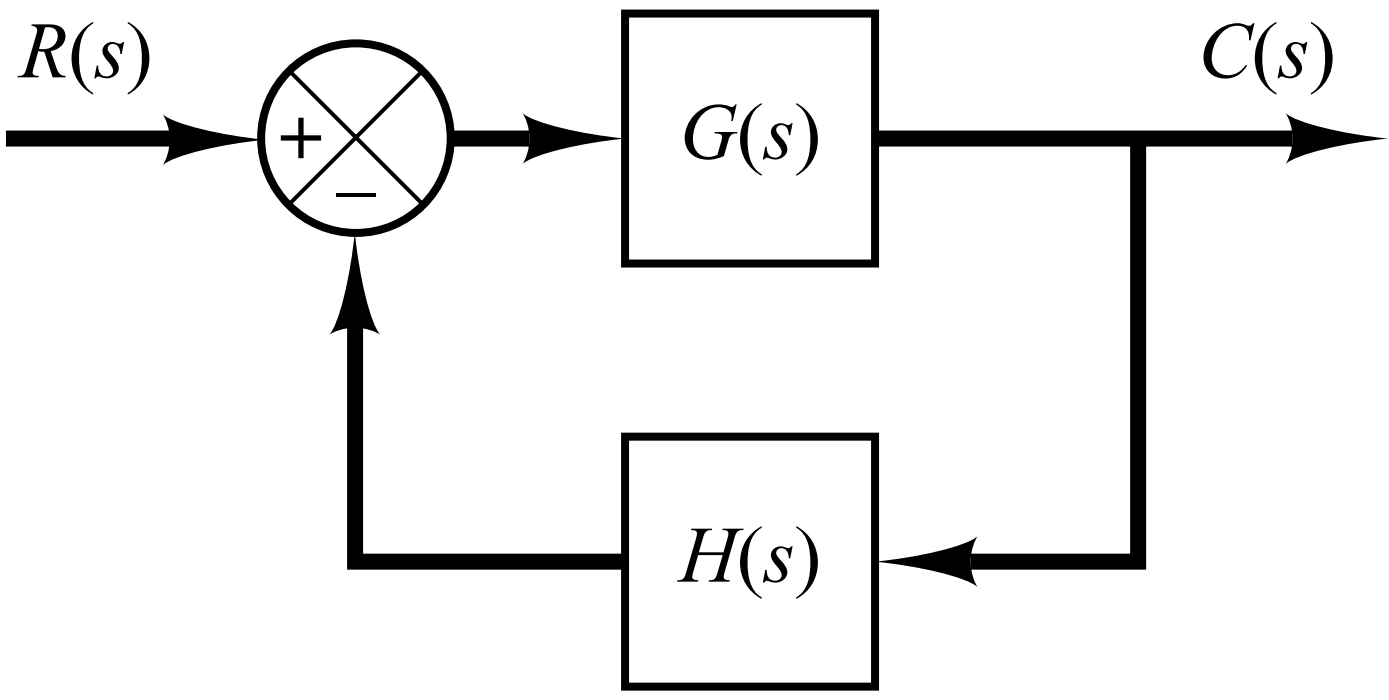
\includegraphics[width=.4\textwidth]{Chapter6/NegativeFeedbackSystem.png} %1.png是图片文件的相对路径
    \caption{基本负反馈系统框图} %caption是图片的标题
    \label{NegativeFeedbackSystem} %此处的label相当于一个图片的专属标志,目的是方便上下文的引用
\end{figure}

假设该系统中$G(s)=\frac{1}{s(s+4)(s^2+4s+20)}$,$H(s)=K_r$,其中$K_r$是非负数,即$K_r=|K_r|e^{j·0}$,则其特征方程为:$1+\frac{|K_r|}{s(s+4)(s^2+4s+20)}=0$,符合根轨迹方程形式,将其改写为:

\begin{equation}
    \begin{cases}
       |K_r|=|s|·|(s+4)|·|(s^2+4s+20)|\\
       -(\phi_s+\phi_{(s+4)}+\phi_{(s^2+4s+20)})=±(2k+1)\pi \quad k=0,1,2...
    \end{cases}
\end{equation}

即$\prod_{j=1}^{m}|(s-z_j)|=1$;\quad$\prod_{i=1}^{n}|(s-p_i)|=|s|·|(s+4)|·|(s^2+4s+20)|$;\quad$\sum_{j=1}^{m}\phi_{z_j}=0$;\quad$\sum_{i=1}^{n}\phi_{p_i}=\phi_s+\phi_{(s+4)}+\phi_{(s^2+4s+20)}$;\quad$\phi_{K_r}=0$;$A(s)=1,B(s)=s(s+4)(s^2+4s+20)$。接下来进行该系统的根轨迹绘制:

根轨迹的起点和终点:

1.绘制所有的(等效)开环传输函数的零极点,即$p_1=0,p_2=-4,P_{3,4}=-2±j4$。

2.绘制各个开环零极点附近的出射角与入射角:$\theta_{s(p=0)}=\pm (2k+1)\pi +0 +0-(0+\frac{63.4}{180}\pi-\frac{63.4}{180}\pi)=\pm (2k+1)\pi$,其他的出射角也同理计算可得。

3.绘制根轨迹的渐近线:渐近线角度为:$\phi_\infty = \frac{±(2k+1)\pi - \phi_{K_r}}{m-n}=\frac{±(2k+1)\pi - 0}{4-0} \quad k=0,1,2...$,渐近线与实轴的交点为$\sigma =\frac{\sum_{i=1}^{n}p_i-\sum_{j=1}^{m}z_j}{n-m}= \frac{-4-2+4j-2-4j}{4}=-2$

根轨迹的中间节点:

4.绘制汇合分离点:因为$B(s)A'(s)-B'(s)A(s)=4s^3+24s^2+72s+80$,所以通过方程$4s^3+24s^2+72s+80=0$求得$s_1=-2,s_{2,3}=-2±j2.45$。通过判断两复根满足相角条件,因此存在三个分离点。

5.绘制与虚轴交点:因为该系统的特征方程为$s^4+8s^3+36s^2+80s+K_r=0$,所以可以得到其劳斯表为:
\begin{equation}
    \begin{matrix}
        s^4&1&36&K_r\\
        s^3&8&80\\
        s^2&208&8K_r\\
        s^1&260-K_r\\
        s^0&8K_r
    \end{matrix}
\end{equation}

只有当$K_r=260$时劳斯表会出现全零行,所以将$K_r=260$带入可得上一行可得辅助方程:$208s^2+8*260=0$,解的$s=±j3.16$

6.绘制根轨迹图:通过将根轨迹的起点、终点和中间节点进行连接绘制出该系统的根轨迹图,如图\ref{RootlocusExample}所示。

\begin{figure}
    \centering
    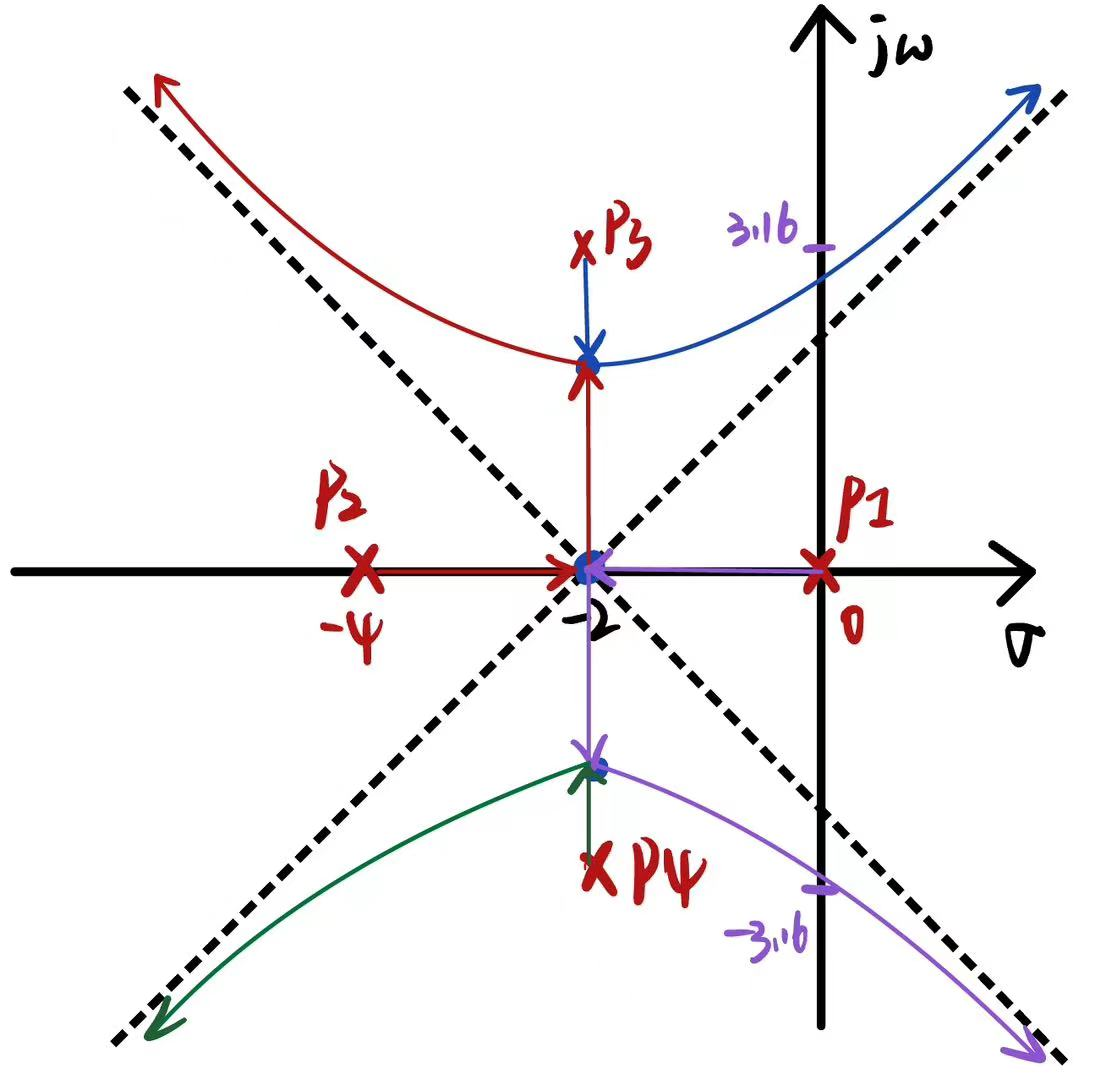
\includegraphics[width=.3\textwidth]{Chapter6/RootlocusExample.jpg} %1.png是图片文件的相对路径
    \caption{特征方程为$1+G(s)H(s)=1+\frac{K_r}{s(s+4)(s^2+4s+20)}=0$的根轨迹图} %caption是图片的标题
    \label{RootlocusExample} %此处的label相当于一个图片的专属标志,目的是方便上下文的引用
\end{figure}

7.确定所需极点对应的$K_r$:通过选择根轨迹上的极点并基于幅值要求得到具体的$K_r$值。

\subsection{正反馈系统的根轨迹绘制}

图\ref{PositiveFeedbackSystem}所示的是一个具备外部反馈的正反馈系统,其中$G(s)$与$H(s)$构成的环路形成了正反馈环路,其传输函数为$\frac{G(s)}{1-G(s)H(s)}$;外部的反馈环路则是用于稳定系统。

\begin{figure}
    \centering
    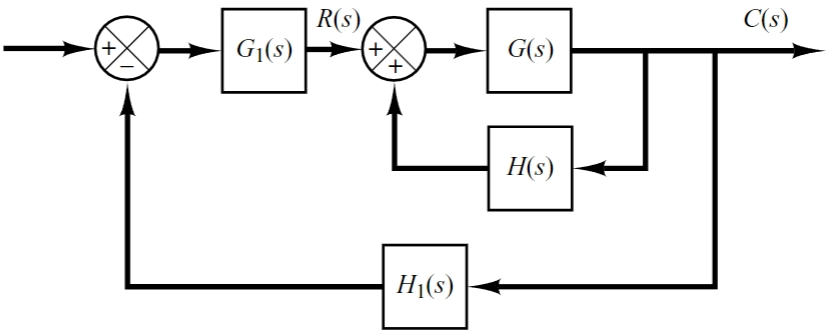
\includegraphics[width=.6\textwidth]{Chapter6/PositiveFeedbackSystem.png} %1.png是图片文件的相对路径
    \caption{具备外部反馈的正反馈系统} %caption是图片的标题
    \label{PositiveFeedbackSystem} %此处的label相当于一个图片的专属标志,目的是方便上下文的引用
\end{figure}

假设正反馈环路中$G(s)=\frac{K(s+2)}{(s+3)(s^2+2s+2)}$,$H(s)=1$,$K$为正数,则特征方程为$1-K·\frac{(s+2)}{(s+3)(s^2+2s+2)}=0$,即$1+K_r·\frac{(s+2)}{(s+3)(s^2+2s+2)}=0$,其中$K_r=(-K)$。则$\prod_{j=1}^{m}|(s-z_j)|=|s+2|$;\quad$\prod_{i=1}^{n}|(s-p_i)|=|s+3|·|s+1-j|·|s+1+j|$;\quad$\sum_{j=1}^{m}\phi_{z_j}=\phi_{(s+2)}$;\quad$\sum_{i=1}^{n}\phi_{p_i}=\phi_{(s+3)}+\phi_{(s+1-j)}+\phi_{(s+1+j)}$;\quad$\phi_{K_r}=\pi$;$A(s)=(s+2),B(s)=(s+3)(s^2+2s+2)$。接下来进行该系统的根轨迹绘制:

1.绘制所有的(等效)开环传输函数的零极点,即$z_1=-2;p_1=-3,p_2=-1+j,p_3=-1-j$。

2.绘制各个开环零极点附近的出射角与入射角:$\theta_{s(p=-1+j)}=\pm (2k+1)\pi +\pi +\frac{\pi}{4}-(\frac{3}{20}\pi+\frac{\pi}{2})=\frac{-2}{5}\pi$,其他的出射角也同理计算可得。

3.绘制根轨迹的渐近线:渐近线角度为:$\phi_\infty = \frac{±(2k+1)\pi - \phi_{K_r}}{m-n}=\frac{±(2k+1)\pi - \pi}{3-1} \quad k=0,1,2...$,渐近线与实轴的交点为$\sigma =\frac{\sum_{i=1}^{n}p_i-\sum_{j=1}^{m}z_j}{n-m}= \frac{(-5)-(-2)}{2}=-1.5$

根轨迹的中间节点:

4.绘制汇合分离点:因为$B(s)A'(s)-B'(s)A(s)=-2s^3-11s^2-20s-10$,所以通过方程$-2s^3-11s^2-20s-10=0$求得$s_1≈-0.802,s_{2,3}≈-2.348±j0.844$。通过判断两复根不满足相角条件,因此只存在一个汇合分离点。

5.绘制与虚轴交点:因为该系统的特征方程为$1s^3+5s^2+(8+K_r)s+(6+2K_r)=0$,所以可以得到其劳斯表为:
\begin{equation}
    \begin{matrix}
        s^3&1&8+K_r\\
        s^2&5&6+2K_r\\
        s^1&\frac{34+3K_r}{5}\\
        s^0&6+2K_r
    \end{matrix}
\end{equation}

只有当$K_r=\frac{-34}{3}$时劳斯表会出现全零行,所以将$K_r=\frac{-34}{3}$带入可得上一行可得辅助方程:$5s^2+(-\frac{50}{3})=0$,解得$s=±\frac{\sqrt{30}}{3}$,即不存在与虚轴的交点。

6.绘制根轨迹图:通过将根轨迹的起点、终点和中间节点进行连接绘制出该系统的根轨迹图,如图\ref{PositiveFeedbackSystemRootlocus}所示。

\begin{figure}
    \centering
    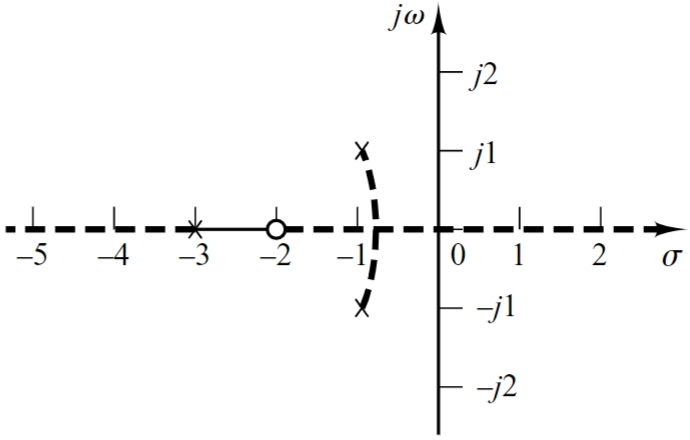
\includegraphics[width=.4\textwidth]{Chapter6/PositiveFeedbackSystemRootlocus.png} %1.png是图片文件的相对路径
    \caption{$G(s)=\frac{K(s+2)}{(s+3)(s^2+2s+2)}$,$H(s)=1$的正反馈系统的根轨迹图} %caption是图片的标题
    \label{PositiveFeedbackSystemRootlocus} %此处的label相当于一个图片的专属标志,目的是方便上下文的引用
\end{figure}

对于特征方程分别为$1-G(s)H(s)$和$1+G(s)H(s)$的正反馈系统和负反馈系统而言,当这两种系统的$G(s)$和$H(s)$相同时,其根轨迹是“连续的”,如图\ref{PosandNegfbsyswithsameG(s)andH(s)}所示,这一段"连续的"完整根轨迹对应的是$K_r$从$-\infty$变化到$\infty$的情况,而正反馈系统和负反馈系统分别的根轨迹则是其中的从$0$到$-\infty$和从$0$到$\infty$的一部分,这与最初推导时的结论是相一致的。

\begin{figure}
    \centering
    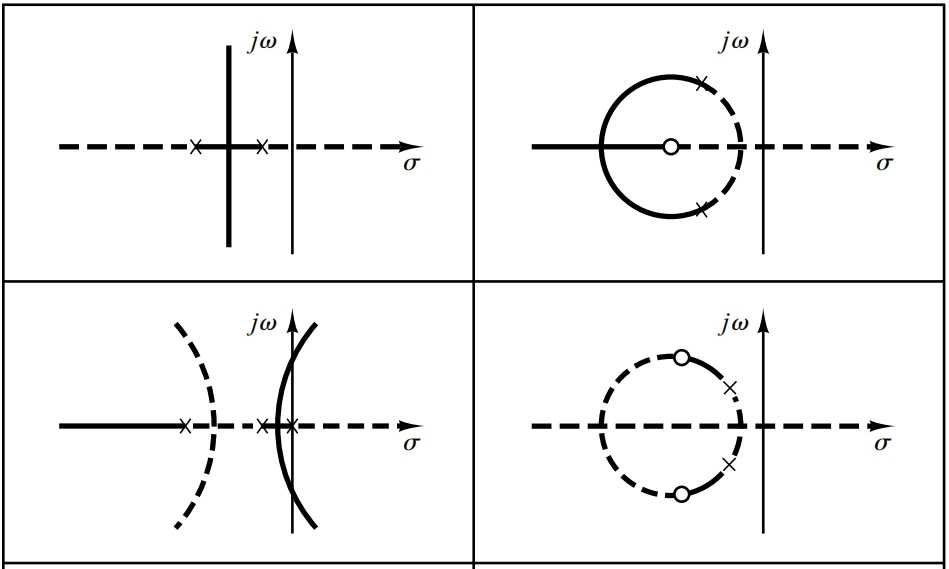
\includegraphics[width=.6\textwidth]{Chapter6/PosandNegfbsyswithsameG(s)andH(s).png} %1.png是图片文件的相对路径
    \caption{特征方程分别为$1-G(s)H(s)$和$1+G(s)H(s)$的正反馈系统和负反馈系统的根轨迹图} %caption是图片的标题
    \label{PosandNegfbsyswithsameG(s)andH(s)} %此处的label相当于一个图片的专属标志,目的是方便上下文的引用
\end{figure}

\subsection{通过根轨迹法进行控制系统设计}
通过上述对根轨迹的定义及推导可知,我们可以通过改变幅值关系和相角关系实现传输函数中极点的改变,例如:通过改变$K_r$的值实现选择根轨迹上不同的点作为传输函数的极点;通过调整系统的(等效)开环零极点$z_i$和$p_j$的位置改变传输函数的根轨迹从而改变传输函数的极点。

当某一个原始系统自身的$K_r$和(等效)开环零极点都不能改变时,如果要改变输出与输入信号之间传输函数的极点位置,就需要额外引入新的变量或(等效)开环零极点从而使得输出与输入信号之间传输函数的极点位置发生变化。具体实现新的变量或(等效)开环零极点引入的部分我们称之为补偿器(Compensator)。

使用这种方法能够使得系统存在我们所需要的极点,但是系统仍旧可能会因此出现其他额外的极点,因此如果我们需要使用这种方法进行系统设计并希望我们的系统符合性能指标,我们就需要保证我们所设计的极点是这个系统的主极点,即其他系统的零极点对系统响应产生的影响足够小。

\begin{formal}
    串联补偿与并联补偿
\end{formal}

补偿可以根据补偿器$G_c(s)$与原始系统$G(s)$的连接方式分为串联补偿(图\ref{SeriesCompensation})和并联补偿(图\ref{ParallelCompensation})。

串联补偿:补偿器$G_c(s)$与原始系统$G(s)$串联连接。

并联补偿:补偿器$G_c(s)$与原始系统$G(s)$并联连接,即补偿器$G_c(s)$处于信号反馈通路上。

一般来说,串联补偿相较于并联补偿更简单,但是串联补偿的补偿器需要通常会需要额外的放大器从而提供增益或隔离(为了降低功耗,一般串联补偿器会被嵌入在前馈路径中能量最低的节点),即选用串联补偿时补偿器的组成元件相较于并联补偿会更多,因为并联补偿是将高电平信号转化为低电平信号,额外的放大器是不必要的。

简而言之,串联补偿容易实现,并联补偿所用元件更少。

\begin{figure}
    \centering
    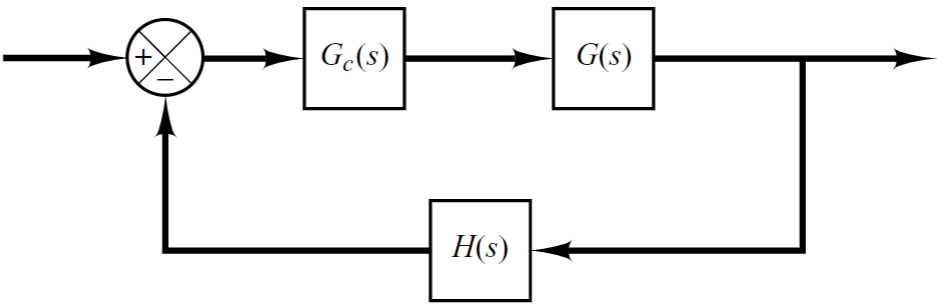
\includegraphics[width=.6\textwidth]{Chapter6/SeriesCompensation.png} %1.png是图片文件的相对路径
    \caption{串联补偿} %caption是图片的标题
    \label{SeriesCompensation} %此处的label相当于一个图片的专属标志,目的是方便上下文的引用
\end{figure}

\begin{figure}
    \centering
    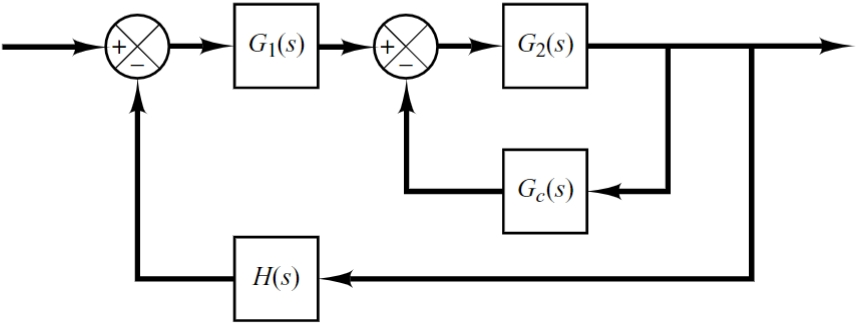
\includegraphics[width=.6\textwidth]{Chapter6/ParallelCompensation.png} %1.png是图片文件的相对路径
    \caption{并联补偿} %caption是图片的标题
    \label{ParallelCompensation} %此处的label相当于一个图片的专属标志,目的是方便上下文的引用
\end{figure}

\begin{formal}
    补偿器的分类
\end{formal}

补偿器主要分为滞后补偿器、超前补偿器和滞后超前补偿器。

我们假定一个系统的传输函数为$G(s)=\frac{Y(s)}{U(s)}$,其中$y(t)\leftrightarrow Y(s)=|Y(s)|e^{j\phi_Y}$、$u(t)\leftrightarrow U(s)=|U(s)|e^{j\phi_U}$,$G(s)=K_r\frac{\prod_{j=1}^{m}(s-z_j)}{\prod_{i=1}^{n}(s-p_i)}=|K_r|e^{j\phi_{K_r}}\frac{\prod_{j=1}^{m}|s-z_j|e^{j\phi_{z_j}}}{\prod_{i=1}^{n}|s-p_i|e^{j\phi_{p_i}}}$,则$\frac{Y(s)}{U(s)}=K_r\frac{\prod_{j=1}^{m}(s-z_j)}{\prod_{i=1}^{n}(s-p_i)}$,(虽然这里的零点和极点也都是用$z_j$和$p_i$进行表示的,但它们并不能被称为(等效)开环零极点,只有根轨迹方程中的$z_j$和$p_i$可以被称为(等效)开环零极点)即:
\begin{equation}
    \frac{|Y(s)|e^{j\phi_Y}}{|U(s)|e^{j\phi_U}}=|K_r|e^{j\phi_{K_r}}\frac{\prod_{j=1}^{m}|s-z_j|e^{j\phi_{z_j}}}{\prod_{i=1}^{n}|s-p_i|e^{j\phi_{p_i}}}
\end{equation}

以幅值和相位展开上式可得:

\begin{equation}
    \begin{cases}
       \frac{|Y(s)|}{|U(s)|}=|K_r|\frac{\prod_{j=1}^{m}|s-z_j|}{\prod_{i=1}^{n}|s-p_i|}\\
       \phi_Y-\phi_U=\sum_{j=1}^{m}\phi_{z_j}-\sum_{j=1}^{n}\phi_{p_i}+\phi_{K_r}
    \end{cases}
\end{equation}

根据极坐标的定义可知$\phi_{z_j}$为逆时针条件下$\vv{s-z_j}$与正半轴的夹角,$\phi_{p_i}$为逆时针条件下$\vv{s-p_i}$与正半轴的夹角,如图\ref{angleofziandpj}所示,$\phi_{K_r}$为逆时针条件下$\vv{K_r}$与正半轴的夹角,由于一般情况下$K_r$为常数,因此$\phi_{K_r}$一般取$0$或$\pi$。

\begin{figure}
    \centering
    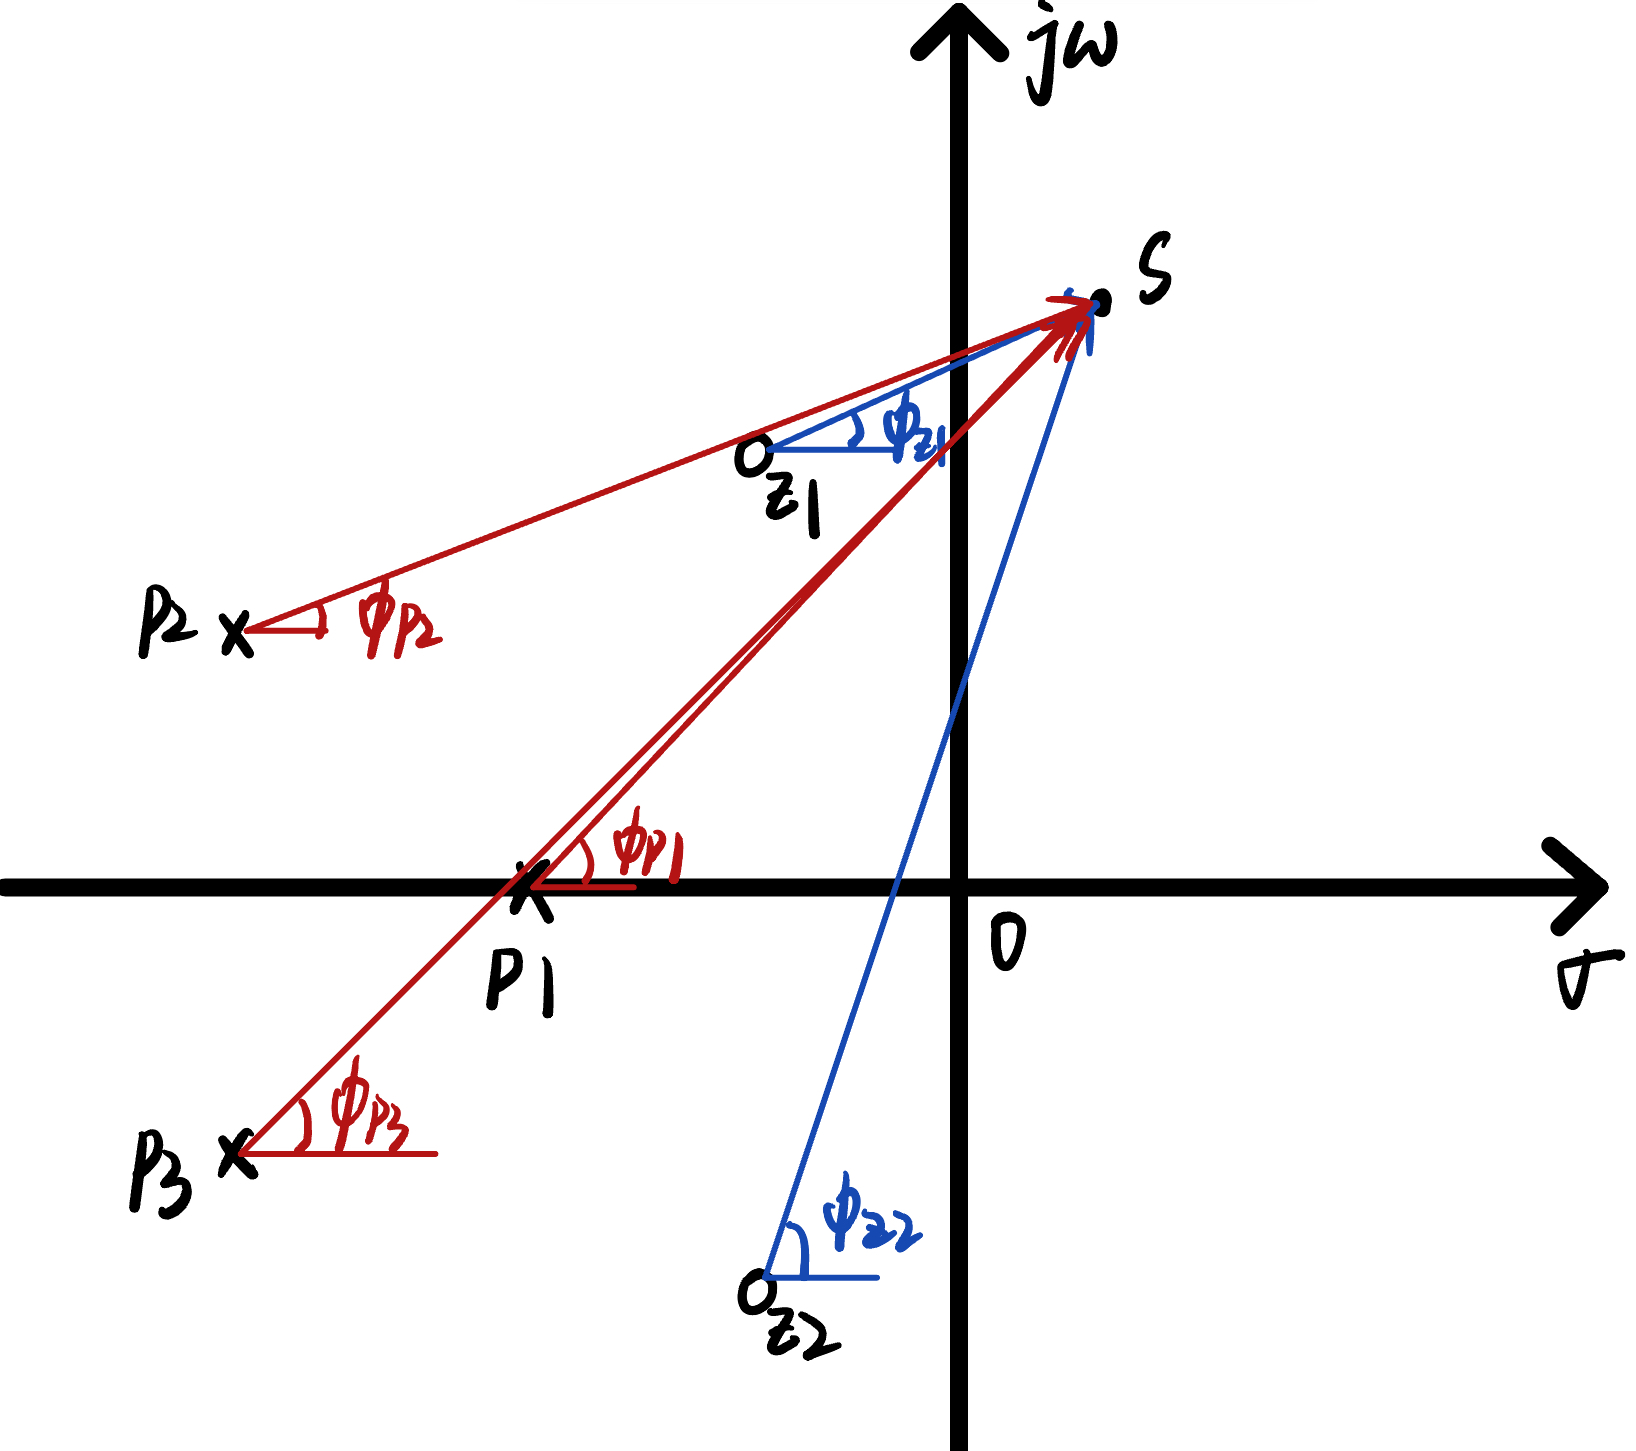
\includegraphics[width=.4\textwidth]{Chapter6/angleofziandpj.jpg} %1.png是图片文件的相对路径
    \caption{s平面内$\phi_{z_j}$和$\phi_{p_i}$示意图} %caption是图片的标题
    \label{angleofziandpj} %此处的label相当于一个图片的专属标志,目的是方便上下文的引用
\end{figure}

根据前文中对傅里叶变化和拉普拉斯变换的分析可知,$Y(s)$和$U(s)$实际上分别代表了函数$y(t)e^{-\sigma t}$和$u(t)e^{-\sigma t}$的傅里叶变换,因此$\frac{|Y(s)|}{|U(s)|}$代表了函数$y(t)e^{-\sigma t}$和$u(t)e^{-\sigma t}$的谐波分量的幅值密度比(即幅值比),而$\phi_Y-\phi_U$代表了函数$y(t)e^{-\sigma t}$和$u(t)e^{-\sigma t}$的谐波分量的相位差。

因此当$s$取虚轴$j\omega$上的值时,即$\sigma=0$时,此时得到的$\frac{|Y(s=j\omega)|}{|U(s=j\omega)|}$就是函数$y(t)$和$u(t)$的谐波分量的幅值密度比(即幅值比),$[\phi_Y-\phi_U]|_{s=j\omega}$就是函数$y(t)$和$u(t)$的谐波分量的相位差。

相应的,此时的$[\phi_{z_j}]|_{s=j\omega}$和[$\phi_{p_i}]|_{s=j\omega}$则如图\ref{angleofziandpj(σ=0)}所示。

因此我们可以总结出如下结论:

\begin{formal}
    输入输出信号相位差图示法:
\end{formal}

当我们观察输出和输入信号之间的相位关系时,我们只需要获得系统的零极点与虚轴上某一点的夹角大小就可以求得输出和输入信号对应角频率(这个角频率大小等于虚轴上所选的点的值)谐波分量之间的相位差,即得到系统对于对应角频率(这个角频率大小等于虚轴上所选的点的值)谐波分量的相移特性。

\begin{figure}
    \centering
    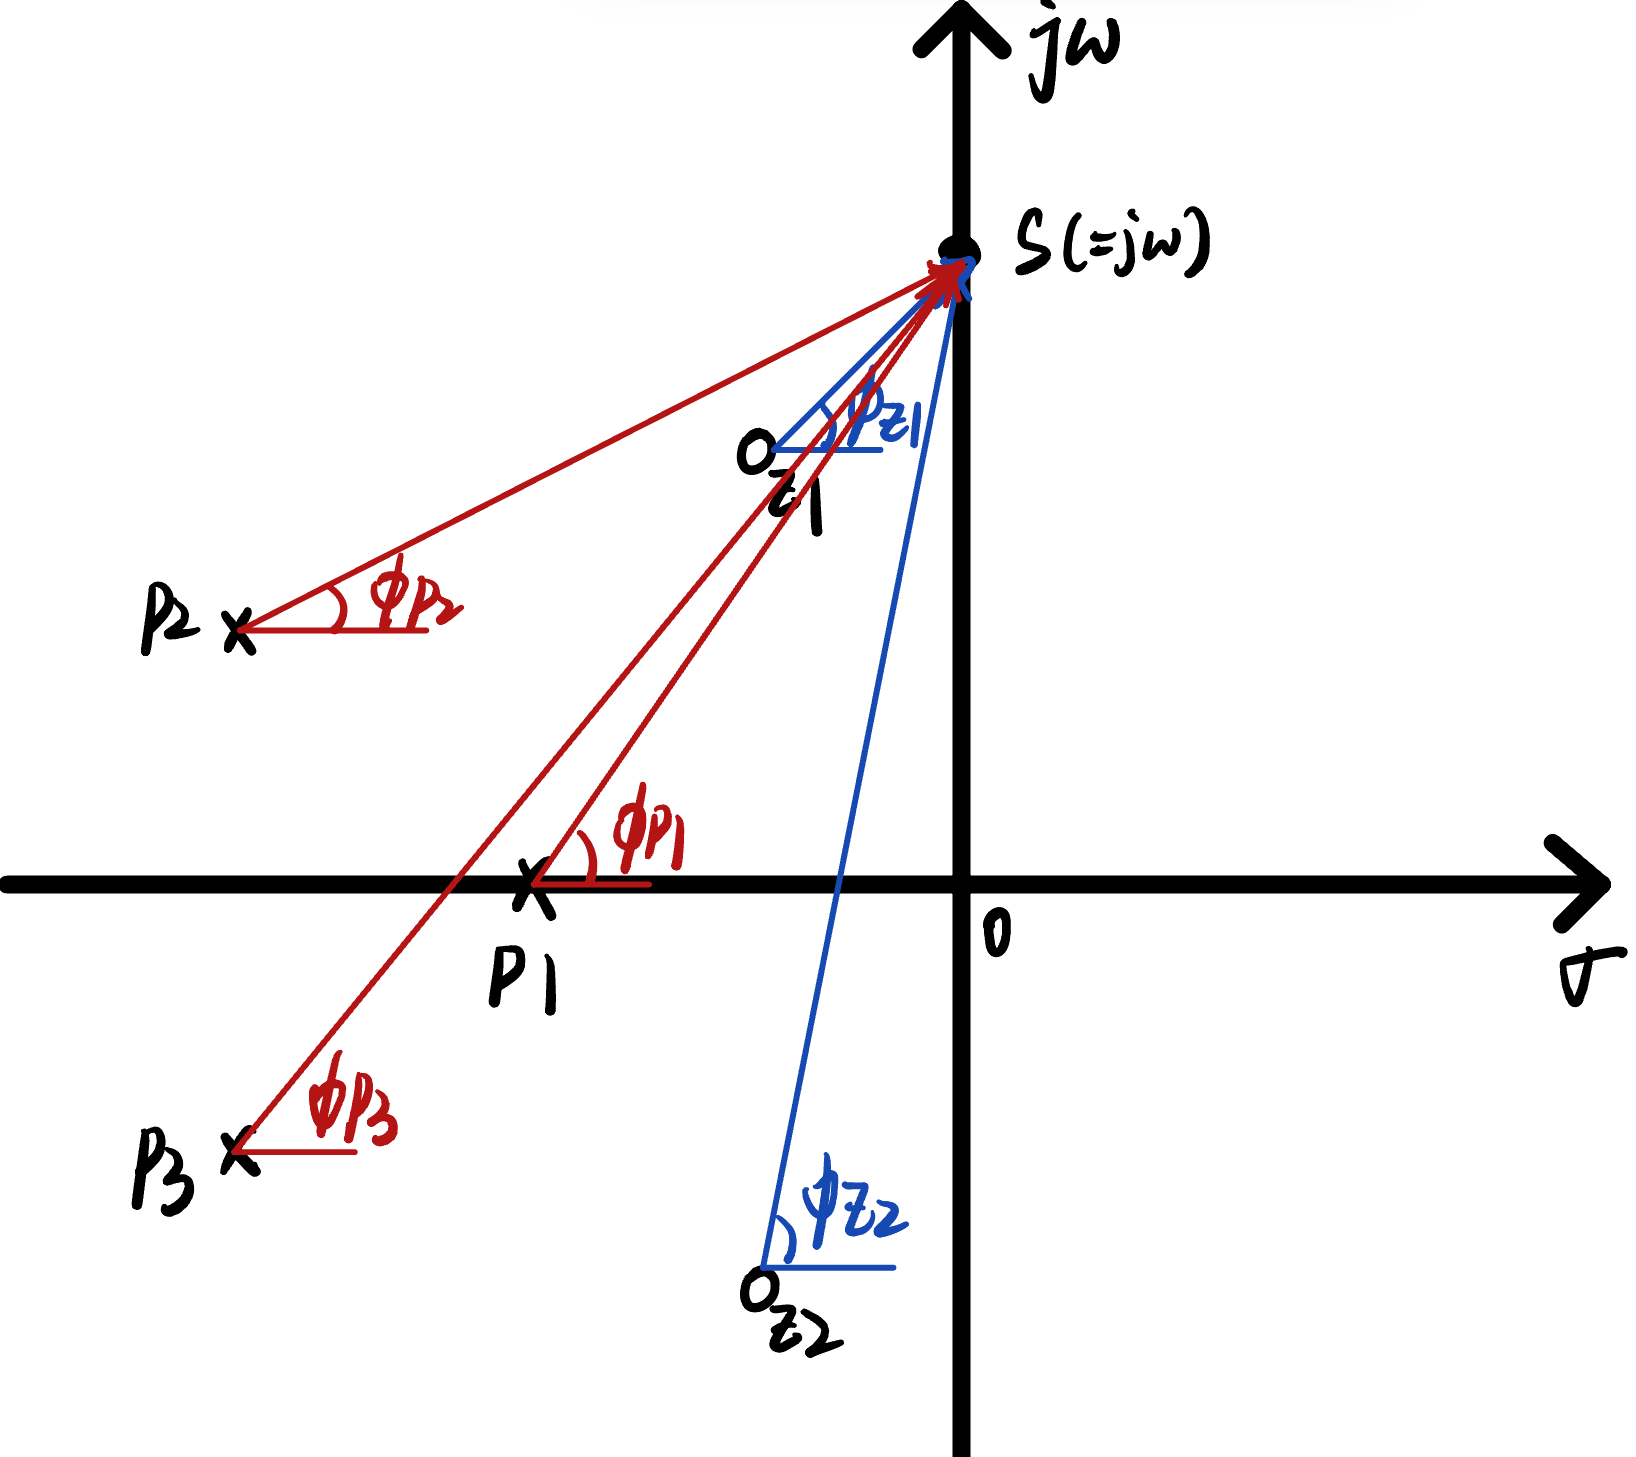
\includegraphics[width=.4\textwidth]{Chapter6/angleofziandpj(σ=0).jpg} %1.png是图片文件的相对路径
    \caption{当$\sigma=0$时s平面内$\phi_{z_j}$和$\phi_{p_i}$示意图} %caption是图片的标题
    \label{angleofziandpj(σ=0)} %此处的label相当于一个图片的专属标志,目的是方便上下文的引用
\end{figure}

通过上述分析我们发现,当$[\sum_{j=1}^{m}\phi_{z_j}-\sum_{j=1}^{n}\phi_{p_i}+\phi_{K_r}]|_{s=j\omega}>0$时,$\frac{|Y(s=j\omega)|}{|U(s=j\omega)|}>0$,输出信号谐波分量的相位超前于输入信号谐波分量的相位,我们称输出信号谐波分量和输入信号谐波分量相位关系满足这种情况的补偿器为超前补偿器。

当$[\sum_{j=1}^{m}\phi_{z_j}-\sum_{j=1}^{n}\phi_{p_i}+\phi_{K_r}]|_{s=j\omega}<0$时,$\frac{|Y(s=j\omega)|}{|U(s=j\omega)|}<0$,输出信号谐波分量的相位滞后于输入信号谐波分量的相位,我们称输出信号谐波分量和输入信号谐波分量相位关系满足这种情况的补偿器为滞后补偿器。

当虚轴上值较小区域$[\sum_{j=1}^{m}\phi_{z_j}-\sum_{j=1}^{n}\phi_{p_i}+\phi_{K_r}]|_{s=j\omega}<0$,即$\frac{|Y(s=j\omega)|}{|U(s=j\omega)|}<0$,输出信号谐波分量的相位滞后于输入信号谐波分量的相位;当虚轴上值较大区域$[\sum_{j=1}^{m}\phi_{z_j}-\sum_{j=1}^{n}\phi_{p_i}+\phi_{K_r}]|_{s=j\omega}>0$,即$\frac{|Y(s=j\omega)|}{|U(s=j\omega)|}>0$,输出信号谐波分量的相位超前于输入信号谐波分量的相位,此时低频区域内输出信号谐波分量的相位滞后于输入信号谐波分量的相位,高频区域内输出信号谐波分量的相位超前于输入信号谐波分量的相位,我们称输出信号谐波分量和输入信号谐波分量相位关系满足这种情况的补偿器为滞后超前补偿器。

正如前文所述,补偿器$G_c(s)$会以串联或并联的方式与原系统$G(s)$相接,此时如果$G_c(s)$出现在补偿后系统的根轨迹方程中,那么$G_c(s)$就会提供额外的(等效)开环传输函数的零极点,从而使得补偿后系统的根轨迹相较于补偿前系统的根轨迹发生变化。

\begin{formal}
    (等效)开环传输函数极点增多的影响:(等效)开环传输函数极点的增多会使得新系统的根轨迹相较于原系统更靠右,使得新系统的相对稳定性更差,并使得响应的建立(settling of response)更慢。(等效)开环传输函数零点增多对根轨迹的影响如图\ref{effectofadditionalopenlooppolesonrootlocus}所示。
\end{formal}

\begin{figure}
    \centering
    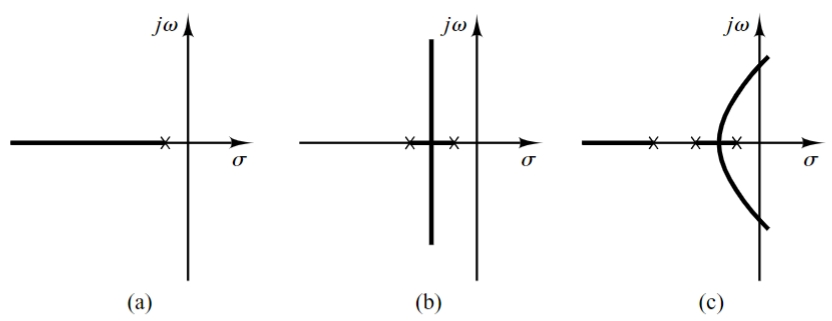
\includegraphics[width=.5\textwidth]{Chapter6/effectofadditionalopenlooppolesonrootlocus.png} %1.png是图片文件的相对路径
    \caption{添加了(等效)开环传输函数极点前后根轨迹对比图} %caption是图片的标题
    \label{effectofadditionalopenlooppolesonrootlocus} %此处的label相当于一个图片的专属标志,目的是方便上下文的引用
\end{figure}

\begin{formal}
    (等效)开环传输函数零点增多的影响:(等效)开环传输函数零点的增多使得新系统的根轨迹相较于原系统更靠左,使得系统更稳定,并加速响应的建立(settling of response)。(等效)开环传输函数零点增多对根轨迹的影响如图\ref{effectofadditionalopenloopzerosonrootlocus}所示。
\end{formal}

\begin{figure}
    \centering
    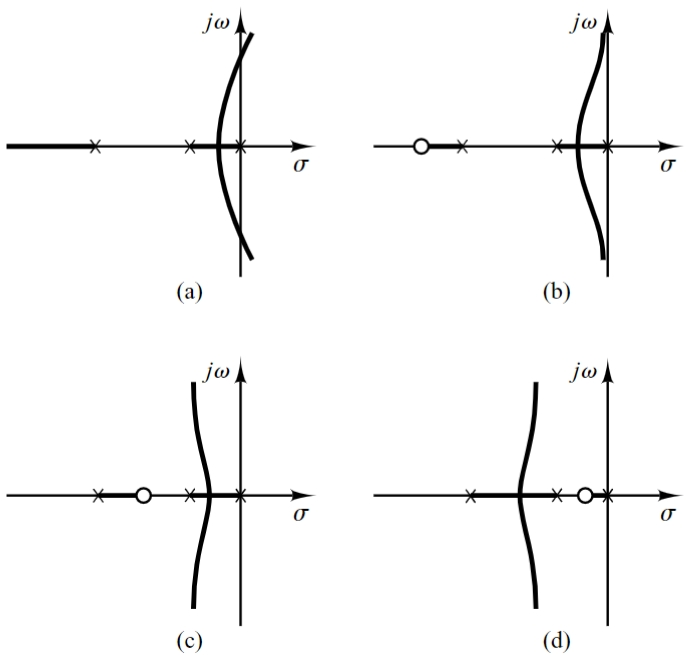
\includegraphics[width=.4\textwidth]{Chapter6/effectofadditionalopenloopzerosonrootlocus.png} %1.png是图片文件的相对路径
    \caption{添加了(等效)开环传输函数零点前后根轨迹对比图} %caption是图片的标题
    \label{effectofadditionalopenloopzerosonrootlocus} %此处的label相当于一个图片的专属标志,目的是方便上下文的引用
\end{figure}

\subsection{超前补偿器}
\begin{figure}
    \centering
    \includegraphics[width=.4\textwidth]{Chapter6/leadorlagcompensator.png} %1.png是图片文件的相对路径
    \caption{相位关系随$R_1C_1$与$R_2C_2$的大小关系变化的电路} %caption是图片的标题
    \label{leadorlagcompensator} %此处的label相当于一个图片的专属标志,目的是方便上下文的引用
\end{figure}

图\ref{leadorlagcompensator}所示的电路的传输函数为:
\begin{equation}
    \frac{E_o(s)}{E_i(s)}=K_c\frac{s+\frac{1}{T}}{s+\frac{1}{\alpha T}}\label{TransferFunctionofleadorlagcompensator}
\end{equation}

其中$T=R_1C_1$,$\alpha T=R_2C_2$,$K_c=\frac{R_4C_1}{R_3C_2}$,即$K_c\alpha =\frac{R_2R_4}{R_1R_3}$,$\alpha =\frac{R_2C_2}{R_1C_1}$。

这个电路的dc增益为$|K_c\frac{s+\frac{1}{T}}{s+\frac{1}{\alpha T}}|_{s=0}=K_c\alpha =\frac{R_2R_4}{R_1R_3}$。(当$\sigma=0$时,即$s=j\omega$时,传输函数等于输出信号的傅里叶变化与输入信号的傅里叶变换之比,此时传输函数的幅值表达的是输出信号与输入信号对应角频率的谐波分量的幅值密度比(即幅值比),此时若取$j\omega=0$,得到的是角频率为0的谐波分量之间的幅值比,即直流分量的幅值比,即dc增益。总而言之,$s=0$时的传输函数的幅值为该系统的dc增益)

从等式\ref{TransferFunctionofleadorlagcompensator}中可以看出,当$R_1C_1>R_2C_2$时(即$\alpha < 1$)时,由于零点相较于极点更靠近虚轴,因此$[\phi_z]|_{s=j\omega}>[\phi_j]|_{s=j\omega}$,此外$[\phi_{K_r}]|_{s=j\omega}=0$,所以$[\sum_{j=1}^{m}\phi_{z_j}-\sum_{j=1}^{n}\phi_{p_i}+\phi_{K_r}]|_{s=j\omega}>0$,所以此时该电路是超前电路,其零极点配置如图\ref{configurationofpolesandzerosofleadorlagcompensator}(a)所示。

当$R_1C_1<R_2C_2$时(即$\alpha > 1$)时,同理可得
该电路是个是个滞后电路,其零极点配置如图\ref{configurationofpolesandzerosofleadorlagcompensator}(b)。

\begin{figure}
    \centering
    \includegraphics[width=.4\textwidth]{Chapter6/configurationofpolesandzerosofleadorlagcompensator.png} %1.png是图片文件的相对路径
    \caption{相位关系随$R_1C_1$与$R_2C_2$的大小关系变化的电路的零极点配置图} %caption是图片的标题
    \label{configurationofpolesandzerosofleadorlagcompensator} %此处的label相当于一个图片的专属标志,目的是方便上下文的引用
\end{figure}

\begin{formal}
    串联补偿——基于根轨迹方法的超前补偿技术
\end{formal}

当指标以时域量(例如:阻尼比、理想的闭环主极点的无阻尼自然频率、最大超调量、上升时间、建立时间等)给出时,超前补偿是一个非常好的方法,这是得益于超前补偿会对系统的根轨迹进行改动从而使得补偿后的系统能够得到理想的极点从而实现时域指标。

超前补偿器通常是串联补偿,如图\ref{LeadCompensationSystem}所示,具体关于如何设计出能够使得闭环主极点处于理想位置的超前补偿电路的流程如下文所述:
\begin{enumerate}
    \item 根据性能指标确定补偿后闭环主极点所处于的理想位置。
    \item 画出未补偿前的系统的根轨迹图,先确认是否能够通过调整现有系统中的某些参数使得系统的主闭环极点能够处于理想位置。如果不能,计算理想位置与未补偿时的(等效)开环零极点之间所成的相角大小,再根据相角关系确定使得理想极点位置处于根轨迹上所需的额外相角$\phi$,这个额外的相角$\phi$则是通过超前补偿器带来的额外的(等效)开环零极点进行提供。
    \item 假定超前补偿系统的传输函数为:
    \begin{equation}
        G_c(s)=K_c\frac{s+\frac{1}{T}}{s+\frac{1}{\alpha T}},\quad (0<\alpha<1)
    \end{equation}
    其中$\alpha$和$T$是通过额外相角$\phi$确定的,$K_c$是通过所需的开环增益决定的。
    \item 如果静态误差常数未被给出指标,则根据额外相角$\phi$确定超前补偿器的零极点的位置。如果没有其他指标限制,尽量将$\alpha$的值设定的越大越好,$\alpha$越大$K_v$越大($K_v$越大斜坡函数作为输入信号时的静态误差越小):$K_v=\lim_{s\rightarrow 0}sG_c(s)G(s)=K_c\alpha\lim_{s\rightarrow 0}G_c(s)$
    \item 通过幅值条件确定补偿后的系统的闭环极点处于理想位置时所需的$K_c$的值
\end{enumerate}

当按照上述步骤将超前补偿器设计完成后,需要检查是否所有的指标都满足了要求,如果有指标未被满足,则需要重复上述设计过程。

从上述第四步可以看出,超前补偿器对于静态误差常数的调整能力有限,因此如果需要较大稳态误差常数,我们则需要级联一个滞后补偿器,或是将超前补偿器改为滞后超前补偿器。

由于在上述过程中我们实际上只是保证了补偿后的系统的闭环极点中会包含我们最初选定的理想极点,但这个理想极点并不一定就是补偿后系统的主闭环极点。因此如果出现最初选定的理想极点并非补偿后系统的主闭环极点的情况,我们就需要再重新选定理想极点并重新设计补偿器。

\begin{figure}
    \centering
    \includegraphics[width=.4\textwidth]{Chapter6/LeadCompensationSystem.png} %1.png是图片文件的相对路径
    \caption{串联超前补偿系统} %caption是图片的标题
    \label{LeadCompensationSystem} %此处的label相当于一个图片的专属标志,目的是方便上下文的引用
\end{figure}

\begin{figure}
    \centering
    \includegraphics[width=.6\textwidth]{Chapter6/ExampleofLeadCompensation_originalsystem.png} %1.png是图片文件的相对路径
    \caption{原始系统} %caption是图片的标题
    \label{ExampleofLeadCompensation_originalsystem} %此处的label相当于一个图片的专属标志,目的是方便上下文的引用
\end{figure}

图\ref{ExampleofLeadCompensation_originalsystem}(a)所示的是一个未经补偿的系统,在本章中我们将未经补偿的系统称为“原始系统”,将经过补偿器补偿的系统称为“补偿后的系统”;图\ref{ExampleofLeadCompensation_originalsystem}(b)所示的是这个原始系统的根轨迹。

从图\ref{ExampleofLeadCompensation_originalsystem}(a)可知该原始系统的闭环传输函数为:
\begin{equation}
    \begin{split}
        \frac{C(s)}{R(s)}&=\frac{10}{s^2+s+10}\\
        &=\frac{10}{(s+0.5+j3.1225)(s+0.5-j3.1225)}  
    \end{split}
\end{equation}

所以该原始系统的闭环极点位于:$s=-0.5\pm j3.1225$,这对原始系统的闭环极点对应的阻尼比是$\zeta = (1/2)/\sqrt{10}=0.1581$,这对原始系统的闭环极点对应的无阻尼自然频率是$\omega_n=\sqrt{10}=3.1623rad/sec$。由于阻尼比非常小,因此在这个原始系统的阶跃响应中会有非常大的超调量并且响应也会不理想。

\begin{figure}
    \centering
    \includegraphics[width=.6\textwidth]{Chapter6/ExampleofLeadCompensation_post-compensatedsystem.png} %1.png是图片文件的相对路径
    \caption{补偿后的系统} %caption是图片的标题
    \label{ExampleofLeadCompensation_post-compensatedsystem} %此处的label相当于一个图片的专属标志,目的是方便上下文的引用
\end{figure}

接下来我们将设计一个超前补偿器对这个原始系统进行补偿,这个超前补偿器将进行串联连接,如图\ref{ExampleofLeadCompensation_post-compensatedsystem}所示,以使得补偿后的系统的主闭环极点的阻尼比为$\zeta=0.5$,无阻尼自然频率为:$\omega_n=3rad/sec$。

1.根据这两个指标值我们可以通过下述方程得到理想的补偿后的系统的主闭环极点:
\begin{equation}
    \begin{split}
        s^2+2\zeta \omega_ns+\omega_n^2&=s^2+3s+9\\
        &=(s+1.5+j2.5981)(s+1.5-j2.5981)
    \end{split}
\end{equation}

即理想的补偿后的系统的主闭环极点为:$s=-1.5\pm j2.5981$。

2.通过原始系统的根轨迹和补偿后的系统的主闭环极点位置我们可以发现,原始系统无法通过调整如增益等参数得到理想的主闭环极点,因此必须通过补偿器实现。

图\ref{ExampleofLeadCompensation_post-compensatedsystem}所示补偿后的系统的闭环传输函数为:$\frac{G_c(s)G(s)}{1+G_c(s)G(s)}$,补偿后的系统的特征方程为:$1+G_c(s)G(s)=0$,即:
\begin{equation}
    1+10K_c\frac{s+\frac{1}{T}}{s(s+1)(s+\frac{1}{\alpha T})}=0
\end{equation}

该特征方程满足根轨迹方程要求,根据$K_c$在该补偿电路中的定义可知其恒为正数,即$\phi_{K_c}=0$,将其展开为幅值条件和相角条件为:

\begin{equation}
    \begin{cases}
       |10K_c|=\frac{|s||s+1||s+\frac{1}{\alpha T}|}{|s+\frac{1}{T}|}\\
       \phi_{z=-\frac{1}{T}}-(\phi_{p=0}+\phi_{p=-1}+\phi_{p=-\frac{1}{\alpha T}})=\pm (2k+1)\pi \quad k=0,1,2...
    \end{cases}
\end{equation}

所以如果理想的补偿后的系统主极点要处于补偿后系统的根轨迹上,那么就必须满足相角条件,即:
\begin{equation}
    [\phi_{z=-\frac{1}{T}}-\phi_{p=-\frac{1}{\alpha T}}]|_{s=-1.5+j2.5981}=\pm (2k+1)\pi+[\phi_{p=0}+\phi_{p=-1}]|_{s=-1.5+j2.5981} \quad k=0,1,2...
\end{equation}

通过计算可得额外相角$\phi=\pm (2k+1)\pi+[\phi_{p=0}+\phi_{p=-1}]|_{s=-1.5+j2.5981}=\pm (2k+1)\pi+2.09439+1.760920231=\pm (2k+1)\pi+3.855311369 \quad k=0,1,2...$,即$\phi=0.713718715 \pm 2k\pi \quad k=0,1,2...$。

3.能够提供这一额外相角的补偿器的零极点组合有无数组。接下来,我们将着重介绍两种组合,第一种是能够尽可能取到最大$\alpha$值的组合;第二种是能够与$G(s)$中的极点进行抵消的组合,其中每种组合都将求解出具体的补偿器的传输函数和响应补偿后的系统的传输函数。

\begin{formal}
    能够尽可能取到最大$\alpha$值的补偿器的零极点组合
\end{formal}

将理想的补偿后的系统的主闭环极点在$s$平面上所处的位置称为点$P$,将原点称为点$O$。先将点$P$与点$O$相连接,记该线段为$PO$;再做一条过点$P$的平行于实轴的水平线,该水平线记为$PA$。如图\ref{largerαconfiguration}所示。随后做出$\angle APO$的角平分线$PB$,其中$B$为角平分线与实轴的交点。之后再绘制$PC$和$PD$分别与$PB$构成角度$\pm \frac{\phi}{2}$,其中$C$和$D$为与实轴的交点。如图\ref{largerαconfiguration}所示。

\begin{figure}
    \centering
    \includegraphics[width=.4\textwidth]{Chapter6/largerαconfiguration.png} %1.png是图片文件的相对路径
    \caption{取到最大$\alpha$值的补偿器的零极点组合} %caption是图片的标题
    \label{largerαconfiguration} %此处的label相当于一个图片的专属标志,目的是方便上下文的引用
\end{figure}


由于补偿器为超前补偿器,因此$D$为超前补偿器的零点,$C$为超前补偿器的极点。由于$PC$和$PD$的夹角为$\phi$,根据三角形的外角等于另外两内角之和可知$\angle PDO=\angle PCD + \phi$,又因为$\angle PDO=\phi_{z=-\frac{1}{T}}$,$\angle PCD=\phi_{p=-\frac{1}{\alpha T}}$,所以$\phi_{z=-\frac{1}{T}} - \phi_{p=-\frac{1}{\alpha T}}=\phi$,即零极点为这组值得超前补偿器能够提供额外相角。

通过第二步可知超前补偿器所需要提供得额外相角为$\phi=0.713718715 \pm 2k\pi \quad k=0,1,2...$,即$\phi = 40.894°$(不考虑周期性),基于上述确定补偿器的零极点组合的步骤我们可以得到补偿器的零点为$-1.9432$,极点为$-4.6458$,即$G(s)$为:
\begin{equation}
    G_c(s)=K_c\frac{s+\frac{1}{T}}{s+\frac{1}{\alpha T}}=K_c\frac{s+1.9432}{s+4.6458}
\end{equation}

4.从上述表达式可知该补偿器的$\alpha$的值为:$\alpha = 1.9432/4.6458 =0.418$

5.由于该补偿后系统的幅值要求为:
\begin{equation}
    |10K_c|=\frac{|s||s+1||s+4.6458|}{|s+1.9432|}
\end{equation}

所以可以求得$K_c=1.2287$,因此超前补偿器$G_c(s)$为:$G_c(s)=1.2287\frac{s+1.9432}{s+4.6458}$。

补偿后系统的开环传输函数为:$G_c(s)G(s)=1.2287\frac{s+1.9432}{s+4.6458}\frac{10}{s(s+1)}$。

补偿后系统的闭环传输函数为:$\frac{C(s)}{R(s)}=\frac{12.287s+23.876}{s^3+5.646s^2+16.933s+23.876}$

补偿后系统的根轨迹如图\ref{largerαrootlocus}所示。

\begin{figure}
    \centering
    \includegraphics[width=.4\textwidth]{Chapter6/largerαrootlocus.png} %1.png是图片文件的相对路径
    \caption{使用取得最大$\alpha$值的零极点组合的补偿器补偿后系统的根轨迹图} %caption是图片的标题
    \label{largerαrootlocus} %此处的label相当于一个图片的专属标志,目的是方便上下文的引用
\end{figure}

通过将补偿后系统的闭环传输函数展开我们可以发现,补偿后的系统的极点有三个,分别为:$s_{p1,2}=-1.5 \pm j2.5981$和$s_{p3}=-2.65$,由于$s_{p3}=-2.65$十分接近补偿后系统的零点$s_{z1}=-1.9342$,因此极点$s_{p3}=-2.65$对于瞬态响应的影响相对小,所以理想的补偿后系统的极点$s_{p1,2}=-1.5 \pm j2.5981$是该补偿后系统的主极点。

该补偿后系统的静态速度误差常数$K_v=\lim_{s\rightarrow 0}sG_c(s)G(s)=5.139$。

\begin{formal}
    能够与$G(s)$中的极点进行抵消的组合
\end{formal}

当我们选择将超前补偿器的零点选在$s=-1$处时,此时等效开环传输函数$G(s)G_c(s)$的分子分母中均会出现$s+1$项,进而相消。

由于超前补偿器的零点选在了$s=-1$处,则根据所需要提供的额外相角可知该补偿器的极点必须位于$s=-3$处,即该补偿器的传输函数为:
\begin{equation}
    G_c(s)=K_c\frac{s+1}{s+3}
\end{equation}

由于补偿后系统的闭环传输函数的幅值条件为:
\begin{equation}
    |K_c\frac{s+1}{s+3}\frac{10}{s(s+1)}|=1
\end{equation}

所以可以求得$K_c=|\frac{s(s+3)}{10}|_{s=-1.5+j2.5981}=0.9$。

因此$G_c(s)=0.9\frac{s+1}{s+3}$,则补偿后系统的开环传输函数为:$G_c(s)G(s)=\frac{9}{s(s+3)}$,补偿后系统的闭环传输函数为:$\frac{C(s)}{R(s)}=\frac{9}{s^2+3s+9}$

补偿后的系统的静态速度误差常数为$K_v=\lim_{s\rightarrow 0}sG_c(s)G(s)=\lim_{s\rightarrow 0}s[\frac{9}{s(s+3)}]=3$

相比之下,第一种组合的$K_v$更小,这也就意味着当输入信号为斜坡函数时,第一种组合的稳态误差更小。此外,尽管不同的组合会带来不同的$K_v$值,但也正如前文所述,不同组合导致的$K_v$的变化幅度较小,因此如何需要较大的$K_v$值,我们就需要级联一个滞后补偿器或将该超前补偿器改为滞后超前补偿器。

\subsection{滞后补偿器}
在超前补偿器中我们发现,超前补偿器可以改善原始系统的瞬态响应特性,但是对静态速率误差常数$K_v$的影响较小,即难以对原始系统的稳态响应进行改善。

因此对于一个具有高性能瞬态响应但是具有较差性能稳态响应的原始系统来说,我们就需要另一种补偿器,以使得在不影响原始系统的高性能瞬态响应的前提下提高其稳态性能,也就是说,这个补偿器要在基本不影响原始系统主闭环极点位置的情况下,提高原始系统的开环增益,从而使得补偿后的系统即拥有理想的主闭环极点,又具有理想的足够大的开环增益。而实现这个目标的补偿器就是滞后补偿器,其连接方式通常是与原始系统进行串联。

为了补偿后的系统还能够拥有原始系统中的主闭环极点,补偿后的系统的根轨迹就一定要经过原始系统中的主闭环极点,即补偿前后的相角条件不能发生改变,补偿器中的零极点不能额外提供相角。

但是做到补偿器中的零极点完全不额外提供相角是较为艰难的,因此我们会允许补偿器中的零极点额外提供较小的相角,以使得补偿后的系统的根轨迹虽然不再经过原始系统中的主闭环极点,但是补偿后的系统仍能拥有近似于原始系统中的主闭环极点的主闭环极点。

为了使得补偿后的系统的主闭环极点相较原始系统中的主闭环极点的偏离程度较小,一般情况下我们会要求滞后补偿器中的零极点额外提供相角在$[-5°,0°]$。

要实现滞后补偿器中的零极点额外提供相角在$[-5°,0°]$内,我们就需要将滞后补偿器中的零极点仿制的十分接近,并且使它们十分靠近原点(是只有图\ref{leadorlagcompensator}中所示的补偿器有这个靠近原点的要求还是都需要?)。

使用了零极点具有上述特点的滞后补偿器进行补偿后的系统的闭环主极点就只会相较于原始系统的闭环主极点有略微的偏移,即瞬态响应也只会有略微的变化。

正如在超前补偿器中所述,图\ref{leadorlagcompensator}是一个相位关系随着$R_1C_1$与$R_2C_2$大小关系变化的补偿器,因此在滞后补偿器中,我们仍可以继续选用图\ref{leadorlagcompensator}所示电路作为滞后补偿器进行使用,其传输函数为:
\begin{equation}
    \frac{E_o(s)}{E_i(s)}=K_c\beta\frac{Ts+1}{\beta Ts+1}=K_c\frac{s+\frac{1}{T}}{s+\frac{1}{\beta T}}
\end{equation}

其中$T=R_1C_1$,$\beta T=R_2C_2$,$\beta=\frac{R_2C_2}{R_1C_1}>1$,$K_c=\frac{R_4C_1}{R_3C_2}$。从中我们可以看到,所有参数的定义都与超前补偿器中的定义一致,只不过对于$\frac{R_2C_2}{R_1C_1}$而言,当其大于$1$时,我们用$\beta$代表它,当其小于$1$时,我们用$\alpha$代表它。

令原始系统的主闭环极点在$s=s_1$处,由于滞后补偿器的零极点十分接近,因此$|s_1+(\frac{1}{T})|≈|s_1+[\frac{1}{(\beta T)}]|$,即:
\begin{equation}
    |G_c(s1)|=|K_c\frac{s_1+\frac{1}{T}}{s_1+\frac{1}{\beta T}}|≈K_c
\end{equation}

为了确保滞后补偿器的角度贡献小,我们需要满足:
\begin{equation}
    -5°<\phi_{z=-\frac{1}{T}}-\phi_{p=-\frac{1}{\beta T}}<0°
\end{equation}

根据补偿后的闭环传输函数的相角关系可知,当滞后补偿器的相角贡献小时,补偿后系统的根轨迹和原始系统的根轨迹基本一致。

在补偿后系统的根轨迹和原始系统的根轨迹基本一致的前提下,根据补偿后的闭环传输函数的幅值关系可知,当$K_c$被设置为约等于1时,将会是原始系统的主闭环极点附近的处于补偿后系统的根轨迹上的值使得补偿后系统的幅值关系得到满足。

综上所述,只要我们将滞后补偿器的相角贡献设置的足够小且将$K_c$设置为约等于1,即滞后补偿器的零极点靠的非常近,那么使用这个滞后补偿器串联补偿后的系统的闭环主极点仍将约等于原始系统的闭环主极点。(这个结论只适用于图\ref{leadorlagcompensator}所示滞后补偿器或具有类似补偿器传输函数的滞后补偿器之中)。

由于补偿后系统的静态速率误差常数为$K_v=\lim_{s\rightarrow 0}sG(s)G_c(s)=\lim_{s\rightarrow 0}G_c(s)\lim_{s\rightarrow 0}sG(s)=K_c\beta \lim_{s\rightarrow 0}sG(s)$,其中$K_c\beta$是补偿器的dc增益。从中我们可以看出补偿后系统的静态速率误差常数具有两个乘积系数$K_c$和$\beta$,由于$K_c$约等于1,因此补偿后系统的静态速率误差常数主要随着$\beta$的增大而增大。

而要在满足滞后补偿器的零极点靠的非常近的前提下取到一个大的$\beta$,则需要一个非常大的$T$的取值,即滞后补偿器的零极点要十分靠近原点。具体的$T$的取值并不关键,只要$T$的大小能够满足“零极点靠的非常近”并且物理上可以实现即可。

滞后补偿器的主要缺点在于,由于滞后补偿器通常会存在一个靠近原点的零点,这将会导致补偿后的系统中存在靠近原点的闭环极点。这个补偿后的系统中的靠近原点的闭环极点和补偿器中的靠近远点的零点将会使得阶跃响应中出现一个小幅值的长尾(a long tail of small amplitude in the step response),从而增长了settling time。

\begin{formal}
    串联补偿——基于根轨迹方法的滞后补偿技术
\end{formal}

\begin{figure}
    \centering
    \includegraphics[width=.4\textwidth]{Chapter6/LagCompensationSystem.png} %1.png是图片文件的相对路径
    \caption{串联滞后补偿系统} %caption是图片的标题
    \label{LagCompensationSystem} %此处的label相当于一个图片的专属标志,目的是方便上下文的引用
\end{figure}

如图\ref{LagCompensationSystem}所示的是一个滞后补偿系统,假定原始系统(即开环传输函数为$G(s)$的闭环系统)的瞬态响应性能已经满足指标要求,但是其稳态响应并未满足指标要求,那么我们就需要按照上文所述的目标设计一个滞后补偿器,这个补偿器的设计流程如下:

\begin{enumerate}
    \item 绘制原始系统(即开环传输函数为$G(s)$的闭环系统)的根轨迹,根据瞬态响应指标定位出原始系统的闭环主极点在原始系统根轨迹上的位置,即确定原始系统的闭环主极点的值。
    \item 假定滞后补偿器的传输函数为:
    \begin{equation}
        G_c(s)=K_c\beta\frac{Ts+1}{\beta Ts+1}=K_c\frac{s+\frac{1}{T}}{s+\frac{1}{\beta T}}
    \end{equation}
    那么使用这个滞后补偿器进行串联补偿后的系统的开环传输函数为:$G_c(s)G(s)$。
    \item 确定特定的静态误差常数,即稳态响应的指标要求。
    \item 确定满足指标要求的静态误差常数的必要增量。
    \item 确定滞后补偿器零极点的位置,以使得其在可以增大特定的静态误差常数的值的同时不会改变原始的根轨迹。(需要注意的是,指标中要求的增益的值和原始系统中增益的值的比值等于补偿器中零点到原点的距离与极点到原点的距离之比)(为什么?)
    \item 画出补偿后系统的新的根轨迹图,根据瞬态响应指标在新的更轨迹图上定位出理想的补偿后系统的闭环极点。
    \item 调整滞后补偿器中$K_c$的值以使得补偿后的系统的闭环主极点位移上一步中的理想位置。
\end{enumerate}

以图\ref{ExampleofLagCompensation_originalsystem}(a)中所示的系统为原始系统为例,我们先对该原始系统进行分析,随后进行相应的滞后补偿器的设计。

\begin{figure}
    \centering
    \includegraphics[width=.6\textwidth]{Chapter6/ExampleofLagCompensation_originalsystem.png} %1.png是图片文件的相对路径
    \caption{原始系统及其闭环根轨迹} %caption是图片的标题
    \label{ExampleofLagCompensation_originalsystem} %此处的label相当于一个图片的专属标志,目的是方便上下文的引用
\end{figure}

图\ref{ExampleofLagCompensation_originalsystem}(a)的系统的前馈传输函数为$G(s)=\frac{1.06}{s(s+1)(s+2)}$,这个系统的闭环传输函数为:
\begin{equation}
    \begin{split}
        \frac{C(s)}{R(s)}&=\frac{1.06}{s(s+1)(s+2)+1.06}\\
        &=\frac{1.06}{(s+0.3307-j0.5864)(s+0.3307+j0.5864)(s+2.3386)}
    \end{split}
\end{equation}

其根轨迹如图\ref{ExampleofLagCompensation_originalsystem}(b)所示,其中主闭环极点为$s=-0.3307 \pm j0.5864$。原始系统主闭环极点的阻尼比为$\zeta = 0.491$,无阻尼自然频率是$0.673rad/sec$,静态速度误差常数是$0.53sec^{-1}$。

现在给出稳态指标要求:在不怎么改变主闭环极点的位置的情况下使得静态速度误差常数$K_v$的值需要在$5sec^{-1}$左右。

1.通过上述分析可知,原始系统的闭环主极点为:$s=-0.3307 \pm j0.5864$。

2.在本例中选用图\ref{leadorlagcompensator}所示电路作为滞后补偿器,其传输函数为:
\begin{equation}
    G_c(s)=K_c\beta\frac{Ts+1}{\beta Ts+1}=K_c\frac{s+\frac{1}{T}}{s+\frac{1}{\beta T}}
\end{equation}

我们选用串联补偿的方式,如图\ref{ExampleofLagCompensation_post-compensatedsystem}所示。补偿后的系统的开环传输函数为:
\begin{equation}
    G_c(s)G(s)=K_c\frac{s+\frac{1}{T}}{s+\frac{1}{\beta T}}\frac{1.06}{s(s+1)(s+2)}
\end{equation}

\begin{figure}
    \centering
    \includegraphics[width=.6\textwidth]{Chapter6/ExampleofLagCompensation_post-compensatedsystem.png} %1.png是图片文件的相对路径
    \caption{滞后比较器串联补偿后的系统} %caption是图片的标题
    \label{ExampleofLagCompensation_post-compensatedsystem} %此处的label相当于一个图片的专属标志,目的是方便上下文的引用
\end{figure}

3.根据指标要求可知,补偿后系统的静态速度误差常数应为$5sec^{-1}$。

4.由于原始系统的静态速度误差常数应为$0.53sec^{-1}$,补偿后系统的静态速度误差常数应为$5sec^{-1}$,因此需要将原始系统的静态速度误差常数放大约十倍。

由于根据上述分析可知当采用如图\ref{leadorlagcompensator}所示系统进行滞后补偿时,补偿后的系统的静态速度误差常数约为原始系统的静态速度误差常数的$\beta$倍,因此在该例中,要满足补偿后的系统的误差常数为$5sec^{-1}$,则$\beta$取$10$。

5.由于图\ref{leadorlagcompensator}所示的滞后补偿器的零点和极点都处于虚轴上,因此只要滞后补偿器提供的角度够小,那么就能保证滞后补偿器的零极点靠的非常近,就能满足补偿后的系统的闭环主极点仍约等于原始系统闭环主极点,即瞬态响应性能基本不受改变的目标。

那么当$\beta$取10时,$T$取值越大越能满足上述要求。为了既能满足要求又能使得滞后补偿器能够实现,我们选择能够使得提供的角度在$[-5°,0°]$之间的$T$,在本例中我们选择$T=20$。

那么因此滞后补偿器的传输函数为$G_c(s)=K_c\frac{s+0.05}{s+0.005}$,即滞后补偿器的零极点分别位于$s=-0.05$和$s=-0.005$处。

6.此时补偿后系统的开环传输函数为$G(s)G_c(s)=K_c\frac{s+0.05}{s+0.005}\frac{1.06}{s(s+1)(s+2)}=\frac{K(s+0.05)}{s(s+0.005)(s+1)(s+2)}$,其中$K=1.06K_c$,其特征方程为:$1+\frac{K(s+0.05)}{s(s+0.005)(s+1)(s+2)}=0$,绘制出该补偿后的闭环系统的根轨迹。

由于补偿后的系统的根轨迹还是略微发生了偏移,因此无法做到瞬态响应的性能与原始系统完全一致,但我们可以使得其中重要的一部分瞬态性能指标保持一致。例如在本例中,我们假定需要保证补偿后的系统的主闭环极点的阻尼比需要和原始系统的主闭环极点的阻尼比相等,那么我们就可以在补偿后的系统的根轨迹上找到我们所需要的补偿后的系统的主闭环极点为:$s_{1,2}=-0.31 \pm j0.55$

7.当补偿后的系统的主闭环极点为:$s_{1,2}=-0.31 \pm j0.55$时,根据补偿后的系统的根轨迹的幅值要求可得$K$为:
\begin{equation}
    \begin{split}
        K&=|\frac{s(s+0.005)(s+1)(s+2)}{s+0.05}|_{s=-0.31+j0.55}\\
        &=1.0235
    \end{split}
\end{equation}

那么$K_c=\frac{K}{1.06}=0.9656$

因此滞后补偿器的传输函数为:$G_c(s)=0.9656\frac{s+0.05}{s+0.005}$。

所以补偿后的系统的开环传输函数为$G_c(s)G(s)=\frac{5.12(20s+1)}{s(200s+1)(s+1)(0.5s+1)}$,补偿后的系统的静态速度误差常数$K_v=\lim_{s\rightarrow 0}sG_c(s)G(s)=5.12sec^{-1}$

得益与滞后补偿器的零极点都处于原点附近,补偿后的系统的根轨迹与原始系统的根轨迹在s平面中的大多数区域中都是基本一致的,但是在原点附近还是会出现根轨迹形状的差异。

补偿器在设计完成后,就需要对补偿后的系统的极点进行验证,以确保理想极点在补偿后的系统中仍是主极点。通过将补偿后的系统的传输函数展开可得其他两个闭环极点为$s_3=-2.326$和$s_4=-0.0549$。

其中$s_3=-2.326$相比于$s_{1,2}=-0.31 \pm j0.55$而言距离虚轴非常远,因此不会对$s_{1,2}=-0.31 \pm j0.55$作为补偿后系统的主极点造成影响。

$s_4=-0.0549$这个极点距离补偿后系统的闭环零点十分接近,因此也不会对$s_{1,2}=-0.31 \pm j0.55$作为补偿后系统的主极点造成影响。

滞后补偿后的系统中会存在一对十分接近的闭环极点和零点的原因:滞后补偿器的添加会使得补偿后的系统相较于原始系统多一个靠近滞后补偿器零点的闭环极点,导致补偿后的系统的阶数上升;此外滞后补偿器的零点也会给补偿后的系统添加一个相同的零点,因此补偿后的系统中会出现一对靠的非常近的闭环零极点,这对闭环零极点将会使得该补偿后的系统的阶跃响应中出现一个小幅度的长尾。

综上所示,在补偿后的系统中$s_{1,2}=-0.31 \pm j0.55$是主闭环极点,瞬态响应将符合预期。对于其他瞬态参数而言,补偿后的系统的主极点的无阻尼自然频率时$0.631rad/sec$相较于原始系统的更小,这意味着补偿后的系统的瞬态响应会略慢于原始系统,补偿后的系统的阶跃响应的最大超调量将会相较于原始系统而增加。

\subsection{滞后超前补偿器}

超前补偿后的系统相较于原始系统的响应更快,稳定更好;滞后补偿后的系统相较于原始系统的稳态响应更准确,但是响应的速度变慢了。

如果我们想要同时改善原始系统的稳态响应和瞬态响应,那么我们就同时需要超前补偿器和滞后补偿器,这种情况下相较于超前补偿器和滞后补偿器都作为独立单元进行补偿,一体化的滞后超前补偿器相对而言更经济便宜。

\begin{figure}
    \centering
    \includegraphics[width=.6\textwidth]{Chapter6/leadandlagcompensator.png} %1.png是图片文件的相对路径
    \caption{滞后超前补偿器} %caption是图片的标题
    \label{leadandlagcompensator} %此处的label相当于一个图片的专属标志,目的是方便上下文的引用
\end{figure}

图\ref{leadandlagcompensator}所示的是一种滞后超前补偿器电路,这个滞后超前补偿器的传输函数为:
\begin{equation}
    \frac{E_o(s)}{E_i(s)}=K_c\frac{(s+\frac{1}{T_1})(s+\frac{1}{T_2})}{(s+\frac{\gamma}{T_1})(s+\frac{1}{\beta T_2})}
\end{equation}

其中$\gamma=\frac{R_1+R_3}{R_1}>1$,$\beta=\frac{R_2+R_4}{R_2}>1$,$K_c=\frac{R_2R_4R_6}{R_1R_3R_5}\frac{R_1+R_3}{R_2+R_4}$

令$K_c=K_{c1}·K_{c2}$,则这个滞后超前补偿器的传输函数可以改写为:
\begin{equation}
    \frac{E_o(s)}{E_i(s)}=K_{c1}\frac{(s+\frac{1}{T_1})}{(s+\frac{\gamma}{T_1})}·K_{c2}\frac{(s+\frac{1}{T_2})}{(s+\frac{1}{\beta T_2})}
\end{equation}

从传输函数中可以看出,该“滞后超前补偿器”系统的传输函数等价于“超前补偿器和滞后补偿器串联”系统的传输函数,因此只要求得所需的“超前补偿器和滞后补偿器串联”系统中每项的参数就可以求得该“滞后超前补偿器”系统中每项的参数。

其中“超前补偿器和滞后补偿器串联”系统的参数可以分为先求超前补偿器中的参数再求滞后补偿器中的参数两步,这两步分别对应了上述两节中关于超前补偿器和滞后补偿器设计的部分。

一般来说我们会先保证补偿后的系统拥有正确的极点,即满足瞬态响应需求,再保证补偿后的系统满足稳态响应需求,因此我们会先对超前补偿器的参数进行设计,再对滞后补偿器的参数进行设计,其设计的流程简而言之为:先按照超前补偿的流程对原始系统进行超前补偿,确定只进行超前补偿使得系统满足瞬态指标时各项参数,在对超前补偿后的满足瞬态指标的系统进一步按照滞后补偿的流程对“超前补偿后的满足瞬态指标的”系统进行滞后补偿,确保瞬态性能变动不大的前提下提高稳态性能。具体如下:

\begin{formal}
    串联补偿——滞后超前补偿器的设计方法
\end{formal}

当$\gamma\neq\beta$时:
\begin{enumerate}
    \item 找出补偿后系统的理想极点的位置。
    \item 根据仅进行了超前补偿的补偿系统的相角条件确定超前补偿部分所需提供的额外相角。
    \item 确定超前补偿部分的零极点组合,并基于零极点组合确定$\gamma$和$T_1$的值。
    \item 根据仅进行了超前补偿的补偿系统的幅值条件确定使得“仅经过超前补偿”的系统的闭环主极点完全位于理想的闭环主极点处时的$K_{c1}$值。通过上述步骤我们得到了一个满足瞬态指标要求的系统,这与超前补偿中所述完全一致。
    \item 根据瞬态响应的指标要求确定将满足瞬态指标要求的系统进行滞后补偿时所需的$\beta$。
    \item 根据“将满足瞬态指标要求的系统进行滞后补偿”后的系统的幅值和相角条件确定$T_2$的值。
    \item 根据某些一定要满足的瞬态指标确定$K_{c2}$的值(即对经历了超前和滞后补偿后的系统的闭环主极点最后进行微调)。
\end{enumerate}

其中第1到第4步与超前补偿器设计的流程完全一致;第5到第7步与滞后补偿器设计的流程完全一致。通过上述步骤我们得到了$K_{c1},K_{c2},T_1,T_2,\gamma,\beta$全部的六个参数的值,通过定义$K_c=K_{c1}·K_{c2}$我们可以求得对应的$K_c$的值。

当$\gamma=\beta$时:

这种情况与上一种最大的区别在于,在$\gamma\neq\beta$时,$\gamma$的值是有所选定的超前补偿部分的零极点组合所确定的,但这组组合有无数种可能,因此$\gamma$可以任取一种组合对应的值;在$\gamma=\beta$时,$\gamma$的取值不再是自由的了,其取值必须跟随$\beta$满足稳态指标要求,因此此时$\gamma$的值是唯一的可以确定的,故而上述设计方向需要进行略微改动。
\begin{enumerate}
    \item 找出补偿后系统的理想极点的位置。
    \item 根据仅进行了超前补偿的补偿系统的相角条件确定超前补偿部分所需提供的额外相角。
    \item 利用$\gamma=\beta$的条件通过瞬态指标得到这种情况下唯一的$\gamma$的值,根据$\gamma$的值和所需提供的额外相角确定$T_1$的值。
    \item 根据仅进行了超前补偿的补偿系统的幅值条件确定使得“仅经过超前补偿”的系统的闭环主极点完全位于理想的闭环主极点处时的$K_{c1}$值。
    \item 根据瞬态响应的指标要求确定将满足瞬态指标要求的系统进行滞后补偿时所需的$\beta$。已经在第三步中实现。
    \item 根据“将满足瞬态指标要求的系统进行滞后补偿”后的系统的幅值和相角条件确定$T_2$的值。
    \item 根据某些一定要满足的瞬态指标确定$K_{c2}$的值(即对经历了超前和滞后补偿后的系统的闭环主极点最后进行微调)。
\end{enumerate}

通过上述步骤我们得到了$K_{c1},K_{c2},T_1,T_2,\gamma,\beta$全部的六个参数的值,通过定义$K_c=K_{c1}·K_{c2}$我们可以求得对应的$K_c$的值。

相比之下$\gamma\neq\beta$的情况相较于$\gamma=\beta$的多了一个可以调节的变量,$\gamma\neq\beta$的情况下补偿后的电路的超调量相较于原始系统的超调量被降低的更多。

综上所述,其实对原始系统进行补偿的本质是:
\begin{itemize}
    \item 瞬态响应补偿:调整原始系统的根轨迹使得补偿后的根轨迹能够通过理想的极点位置,并使得补偿后的系统的闭环主极点恰好是根轨迹上的理想极点,使得补偿后的系统能够满足瞬态响应指标要求。
    \item 稳态响应补偿:在不影响原始系统闭环主极点的前提下使得补偿后的系统的开环增益增大,使得补偿后的系统能够满足稳态响应指标要求。
\end{itemize}

因而无论所采用何种方式、何种系统进行补偿,只要能够实现上述目标,就能实现相应的补偿,具体的与补偿相关的参数则也相应的会在实现上述目标的过程中得到。

但记住超前补偿器适用于瞬态响应补偿、滞后补偿器适用于稳态响应补偿的一般规律能够有效帮助我们快速找到合适的补偿器并进行相应的补偿器设计。


\begin{formal}
    Stop at Chapter 6-9
\end{formal}

\end{document}